% Achard, Gajdos Preuss & Servant -- working copy, converted from the Word revision.
%
% CHANGE MARKING. The Word copy this is converted from is colour-coded against
% "Achard et al R1_v3.docx": text already in that version keeps its own colour, text added
% since is blue, and struck runs are proposed deletions. The three macros below carry that
% marking. For a clean copy, redefine them:
%     \renewcommand{\new}[1]{#1}\renewcommand{\old}[1]{#1}\renewcommand{\del}[1]{}
\documentclass[11pt]{article}
\usepackage[T1]{fontenc}
% Latin Modern rather than the T1 Computer Modern bitmaps: microtype's font expansion
% needs a scalable font, and a TeX Live without cm-super installed fails outright on it.
\usepackage{lmodern}
\usepackage[utf8]{inputenc}
\usepackage[margin=1in]{geometry}
\usepackage{amsmath,amssymb}
\usepackage{graphicx}
\usepackage{array}          % >{...} column prefixes, used by the wide tables
\usepackage{xcolor}
\usepackage[normalem]{ulem}
\usepackage{microtype}
\usepackage{lineno}
\usepackage{hyperref}
% hidelinks, not coloured links: this copy uses colour to mark revisions, and a
% blue \cite in the middle of a red sentence reads as new material rather than as a
% link. Links stay live, they just take the colour of the text around them.
\hypersetup{hidelinks}

% Bibliography: biblatex + biber with the APA style, the same setup note4.tex uses, so
% both documents cite the same Zotero library the same way. This needs biber, not bibtex
% -- see README for the build order.
\usepackage[style=apa]{biblatex}
\DeclareLanguageMapping{english}{english-apa}
\addbibresource{bib.bib}

\definecolor{addcol}{HTML}{1F4E9E}
\definecolor{oldcol}{HTML}{FF0000}
\newcommand{\new}[1]{\textcolor{addcol}{#1}}
\newcommand{\old}[1]{\textcolor{oldcol}{#1}}
\newcommand{\del}[1]{\textcolor{oldcol}{\sout{#1}}}

% The printed reference list now comes from biblatex, so body.tex no longer uses this
% environment. It is kept because references_verbatim.tex -- the APA text exactly as Word
% carried it, which checkbib.py reads -- can be \input to set the two lists side by side.
% \everypar rather than a negative \parindent, which \parskip and the surrounding
% zero-indent setting between them cancel out.
\newenvironment{references}
  % \sloppy is load-bearing here. A DOI is one unbreakable word, so a reference ending
  % in a long one has nowhere to break: without \sloppy, eleven of them overrun the
  % margin, one by 136pt. With it, TeX stretches the spaces instead -- five lines come
  % out loose, the worst being Rogge et al. Loose beats off the page. (xurl was tried;
  % it changed neither count, so it is not here.)
  {\par\sloppy\setlength{\parindent}{0pt}\everypar{\hangindent=0.4in\hangafter=1}}
  {\par}

% The paper numbers its own appendix items A.1-A.10 and refers to them by those labels,
% so LaTeX's section numbers would give the same material two competing numberings.
% The Word original has no section numbers either.
\setcounter{secnumdepth}{0}

\setlength{\parskip}{0.5\baselineskip}
\setlength{\parindent}{0pt}
\renewcommand{\thesection}{\arabic{section}}

\title{Graded Motor-Preparatory Dynamics Preserve Perceptual Decisions over Short Delays}
\date{}

\begin{document}
\linenumbers
\textbf{Graded Motor-Preparatory Dynamics Preserve Perceptual Decisions over Short Delays}

Johan A. Achard\textsuperscript{1}, Thibault Gajdos Preuss\textsuperscript{2}, Mathieu Servant\textsuperscript{1}

\textsuperscript{1} Laboratoire de Recherches Int\'egratives en Neurosciences et Psychologie Cognitive, Institut National de la Sant\'e et de la Recherche M\'edicale, Universit\'e Marie et Louis Pasteur

\textsuperscript{2}  Centre de Recherche en Psychologie et Neuroscience, Centre National de la Recherche Scientifique, Aix-Marseille Universit\'e

Abbreviated title:

Perceptual Decisions over Short Delays

Corresponding Author: \url{mathieu.servant@umlp.fr}

Number of pages: 43

\new{Number of figures: 4 (plus 3 supplementary)}

\new{Number of tables: 2 (plus 1 appendix table and 6 supplementary)}

Number of multimedia and 3D models: 0

\new{Number of words for abstract: 248}

\new{Number of words for introduction: 648}

\new{Number of words for discussion: 1359}

Conflict of interest statement: The authors have no conflicts of interest to  declare.

Acknowledgments:  This work was funded by the European Union (ERC Starting Grant ITDA n$^{\circ}$101039226 allocated to MS). Views and opinions expressed are however those of the author(s) only and do not necessarily reflect those of the European Union or the European Research Council. Neither the European Union nor the granting authority can be held responsible for them.

Data availability: Empirical data and analysis code are freely available on the Open Science Framework  (\url{https://osf.io/86cbw/overview?view\_only=1f47b76612334dc082318a501fda5a4c}).

\new{\textbf{Note on this working copy}}

This version marks changes relative to Achard et al R1\_v3.docx (the manuscript as it stood before the internal working-note integration passes). Text is colored black or red exactly as it was colored in that version, regardless of whether the passage has since been moved elsewhere in the document (red there generally marks a passage added in an earlier revision round, tracked by the authors at the time). Blue text is new: it does not appear anywhere in R1\_v3.docx, whether because it was adapted from the internal working note ``The extended evidence-accumulation model for delayed reports'', written as new connecting material, or is a corrected or updated value (for example in Table 2, Tables S2--S3 and Table A1). Red strikethrough marks text that was present in R1\_v3.docx and that we propose to delete, kept visible here so that co-authors can see what is being removed; text introduced during these passes and later superseded has simply been deleted rather than struck. Color and strikethrough are direct character formatting, not Word revision marks, so this file will not open as a marked-up copy in Word's reviewing pane; a clean copy, and a properly tracked copy if the journal requires one, will be produced separately at submission. This is a working draft for internal review, not the clean copy for resubmission.

\textbf{Abstract}

In delayed perceptual reports, the decision is formed before action is permitted, yet response time from the response signal still depends on sensory evidence. This paradox raises the possibility that evidence accumulation leaves a graded trace in motor preparatory circuits rather than ending in a discrete stored choice. We tested this hypothesis in 22 adults of both sexes (17 women) performing a response-signal random-dot motion task with electroencephalography and electromyography. Participants judged motion direction, withheld the selected response for 3 s, and executed it when the response signal was presented; motion coherence and duration were manipulated. Response time increased when coherence or duration decreased.  Fractionating response time at muscle-activation onset showed that these effects were confined to the premotor period. Muscle activations that did not produce overt responses provided a peripheral readout of motor preparation: they were effector-selective, built up during stimulus presentation at a coherence-dependent rate, and \new{continued to ramp during the stimulus-free delay, but no longer at a coherence-dependent build-up rate.} These results support an account in which accumulated motion evidence is transmitted to motor preparatory circuits, transformed into a sustained state maintaining the selected response, and shaped by temporal preparation before action is permitted. Electroencephalography revealed a hierarchy: mu--beta-band lateralization tracked motion-evidence accumulation and temporal preparation, whereas the lateralized readiness potential tracked temporal preparation and continued to build up toward the response. Thus, delayed decisions are preserved not as discrete stored choices, but as graded motor-preparatory states that remain dynamically regulated until action is permitted.

\textbf{Significance statement}

Perceptual decisions often cannot be reported immediately, yet the brain must preserve them until action is allowed. By combining brain and muscle recordings in humans, we show that, over short delays, information extracted from a stimulus is not simply converted into a fixed choice and released later. Instead, it remains graded in motor preparatory circuits, where it is maintained and adjusted by expectations about when action can occur. Muscle activations too weak to produce overt responses provided an especially sensitive window onto these hidden preparatory states, offering a novel tool for studying how decisions are maintained and regulated before behavior.


\section{Introduction}

Perceptual decision-making transforms sensory information into choices that guide action. Much of the human literature has used paradigms in which participants report a choice as soon as they commit to it  \parencites{forstmannSequentialSamplingModels2016}{oconnellNeurophysiologyHumanPerceptual2021}. This work has motivated neurally informed models in which noisy sensory evidence is accumulated and continuously conveyed to the motor system, allowing candidate actions to be prepared in parallel  \parencites{balsdonSecondaryMotorIntegration2023}{dendauwGatedCascadeDiffusion2024}{kellyNeurocomputationalMechanismsPriorinformed2021}.  However, commitment and action are often separated in time, and it remains unclear how such models extend to decisions whose report must be withheld.

A canonical paradigm for studying perceptual decision-making is the random-dot motion discrimination task, in which observers judge motion direction and report their choice with an eye or hand movement. Recent variants impose a delay between stimulus offset and a response signal (RS), requiring observers to withhold their report until prompted  \parencites{achardExtendingContinuousFlow2025}{MotorCorticalSignals}.  If sensory evidence were converted into a discrete choice that was stored and merely released at the RS, mean response time (RT; measured from RS onset) should be insensitive to earlier stimulus characteristics. Yet mean RT is longer with lower motion discriminability and shorter motion duration. These RT effects persist across delays of up to seven seconds, making incomplete decision formation at RS onset unlikely.

\old{To explain delayed-report behavior, we formalized an extension of recent evidence-accumulation models linking decision} \old{and motor processes} \old{in immediate-report tasks.}  \old{Building on empirical evidence that accumulation can terminate at a bound before externally controlled stim}\old{ulus} \old{offset} \old{\parencite{kianiBoundedIntegrationParietal2008}} \old{and on neural-integrator models in which accumulated information can persist} \old{over} \old{time} \old{\parencite{mazurekRoleNeuralIntegrators2003}}\old{, the model sustains the selected motor-preparatory state once an internal threshold is reached. When motion} \old{processing ends before threshold crossing, it instead sustains the graded state reached at that time.} \old{This account is consistent with recurrent-circuit theories linking evidence accumulation and working-memory} \old{maintenance}  \old{\parencite{wangDecisionMakingRecurrent2008}}\new{, and more broadly with accounts of working memory as action-oriented \parencite{vanedeTurningAttentionOut2023}}\new{.} \old{During the delay, learned temporal regularities can} \old{progressively shape} \old{motor preparation as an} \old{anticipated opportunity to act approaches} \old{\parencites{heidemanTemporalAlignmentAnticipatory2018}{liBetaOscillationsInternal2026}{ramayyaHumanResponseTimes2025}}\new{.}  \old{We therefore considered two models: Model 1 includes only the maintained evidence-dependent motor state, whereas Model 2 additionally in}\old{corporates temporal preparation}\new{.} \old{Downstream gating operates throughout the trial, preventing} \old{motor-preparatory activity} \old{from producing overt action}  \old{\parencite{dendauwGatedCascadeDiffusion2024}}\new{.} \old{The RS engages a distinct stochastic process that accumulates noisy evidence that the signal is present}\new{.} \old{The plausibility of noisy temporal integration for an unambiguous signal is supported by accumulator accounts of one-choice} \old{RT}  \old{\parencites{ratcliffDiffusionModelOnechoice2011}{smithPsychophysicallyPrincipledModels1995}} \old{and by electroencephalographic (EEG) signatures of evidence} \old{accumulation under near-ceiling target-detection conditions}  \old{\parencite{oconnellSupramodalAccumulationtoboundSignal2012}}\new{.} \old{Continuous transmission of the accumulated evidence progressively increases the selected motor state until it overcomes the gate and triggers the response.}  \old{This distinction between maintaining and initiating a motor plan has plausible circuit-level analogues. In mice, subcortical control signals can reshape motor-planning dynamics and promote transitions toward movement} \old{execution} \old{\parencite{inagakiNeuralAlgorithmsCircuits2022}}\new{,} \old{whereas primate population studies indicate that} \old{preparatory activity can occupy output-null dimensions that do not immediately drive mo}\old{tor output} \old{\parencite{churchlandPreparatoryActivityExpansive2024}}\new{.} \old{This} \old{organization can keep a selected action prepared without immediate execution, a separation our model represents in reduced form}\new{.}

\new{Both models predict the same qualitative ordering of mean RT with motion coherence and with stimulus duration, because it follows directly from the shared architecture: the second accumulation's drift is fixed across conditions,} \new{so coherence and duration act on RT only through the level maintained at the end of the first stage, which both raise. Behavior alone therefore cannot distinguish the two models' internal dynamics, and we used EEG measures of effector-selective motor preparation, alongside surface electromyographic (EMG) measures of muscle activation, as additional constraints.}


\section{Materials and Methods}


\subsection{Experimental Procedures}


\subsubsection{Participants}

Twenty-two participants (17 women; mean age = 20.08; range 18--24) took part in the experiment in exchange for a \texteuro{}20 gift card.  The sample size was based on our previous study \parencite[Experiment 2]{achardExtendingContinuousFlow2025}, which provided  strong Bayesian evidence (inclusion Bayes factor > 10) that  stimulus discriminability and duration affect delayed-report latency.  Participants were students at  Universit\'e Marie et Louis Pasteur (France) recruited through online advertisements. All were right-handed, had normal or corrected-to-normal vision, and reported no history of motor, psychiatric, or neurological disorders. Participants were unaware of the study purpose and provided written informed consent. The university research ethics committee approved the study (Agreement CERUBFC-2022-01-18-002).


\subsubsection{Experimental task}

Participants performed a \new{response-signal (RS) variant of the} random-dot motion discrimination task. They judged  whether motion was leftward or rightward, maintained the selected response during a 3-s delay, and reported it \new{when the RS} appeared. Leftward and rightward judgments were reported with the corresponding thumb using two buttons mounted in a rubberized ergonomic grip (Black Box Toolkit).  Motion duration (0.3 or 2 s) and coherence (0\%, 12\%, or 50\%) varied factorially. The 0\% condition contained no net directional evidence and therefore indexed chance-level choices; 12\% and 50\% coherence provided intermediate and high discriminability, respectively.

The stimulus contained white dots (0.05$^{\circ}$ in diameter;  71 dots per frame on average) presented within a virtual circular aperture  (11.78$^{\circ}$ in diameter)  on a black background. On each frame, a proportion of dots moved coherently leftward or rightward at 10.5$^{\circ}$/s, whereas the remaining dots were repositioned randomly. Stimuli were displayed on a 34.42 $\times$ 19.36 cm LCD monitor (1920 $\times$ 1080; 60 Hz) viewed from 75 cm in a dimly lit room. Participants rested their hands on a cushion to minimize incidental muscle activity.

Participants completed 10 blocks of 96 trials, with self-paced breaks between blocks. Within each block, trials were defined by the factorial combination of motion direction, motion coherence, and motion duration (0.3 vs 2  s). Each trial type was presented eight times per block in randomized order, resulting in 160 trials per coherence $\times$ duration condition across the experiment.  The time course of each trial is illustrated in Figure 2A. A colored fixation cross remained at the center of the screen for the duration of the trial. After a variable prestimulus interval (0.6, 0.8, or 1  s, randomly selected on a trial-by-trial basis), the motion  stimulus appeared and was followed by a  3-s delay. A change in fixation color from blue to yellow served as the RS. Participants were instructed to respond as quickly and accurately as possible after this change. If no response was made within 4 s of RS onset, the feedback message "Too late, please respond faster" was displayed for 2  s. If a response occurred before the RS, the feedback message "Too early! Please wait for the color change of the fixation cross" was displayed for 2  s. Feedback messages or valid responses were followed by a 1.5  s inter-trial interval, during which a schematic image of an eye was displayed. Participants were instructed to maintain fixation on the central cross and refrain from blinking  until the eye schematic appeared.  Trials with no response  (0.28\%;  participant range, 0--3.34\%), a response before the RS (1.37\%; range, 0.21--3.33\%), or a RT shorter than  0.2 s (0.32\%; range, 0--2.92\%) were excluded.


\subsubsection{EMG acquisition and preprocessing}

EMG activity from  the \emph{flexor pollicis brevis}, which flexes the thumb at the metacarpophalangeal joint and contributes to flexion at the carpometacarpal joint, was continuously recorded during task performance using two active Ag/AgCl electrodes placed 1 cm apart on the skin over the thenar eminence of each hand.  The electrodes were connected to a BioSemi Active  Two Mk2 biopotential measurement system (sampling rate = 1024 Hz).  After acquisition, the voltage difference between each electrode pair was computed. Left- and right-hand  bipolar EMG signals were then high-pass filtered at  10 Hz using a third-order Butterworth filter to remove slow drifts unrelated to muscle activity, full-wave rectified, and segmented from -0.3 to 9 s relative to stimulus onset.

Muscle activation onsets and offsets were detected using the three-step semi-automatic procedure described in \textcite{achardExtendingContinuousFlow2025}. \old{For each trial and EMG channel, the mean and} \old{standard deviation of the full-wave rectified signal were computed during the 300-ms} \old{prestimulus} \old{period. Candidate muscle-activity periods were identified when signal amplitude exceeded the mean by seven standard deviations.} \old{At this initial detection stage, threshold-defined periods separated by less than 25} \old{ms} \old{were merged into a single candidate burst to prevent brief within-burst drops below the conservative detection threshold from artificially splitting a single activation.}  \old{Candidate bursts were then filtered to limit false detections arising from background noise. Specifically, candidate bursts containing} \old{at most} \old{six above-threshold samples were counted} \old{across the epoch}\old{, and their occurrence rate per second was added to a base minimum of three} \old{above-threshold} \old{samples. Candidate bursts not meeting this adaptive criterion were discarded.}  \new{T}\old{he onset and offset of each} \old{retained} \old{candidate burst were then refined using the integrated-profile method}  \old{\parencites{liuUseIntegratedProfile2016}{santelloControlTimingAmplitude1998}}\new{.}  \old{For each burst, the integrated profile was computed from the cumulative rectified EMG in a window encompassing the burst and adjacent background activity, supplemented with additional} \old{background}  \old{EMG from the beginning and end of the epoch. The overall linear trend of this cumulative signal was then removed; inclusion of the additional background activity reduced the influence of the burst itself on the trend estimate. The resulting profile was smoothed using a 15-ms moving average, and its minimum and subsequent maximum were taken as estimates of burst} \old{onset and offset, respectively}\new{.}  \old{The search for the}\old{se extrema} \old{extended up to 50} \old{ms} \old{before the threshold-defined onset and 50} \old{ms} \old{aft}\old{er the threshold-defined offset}\new{.} \old{For neighboring candidate bursts, the search ranges were truncated at the midpoint of the interval between the threshold-defined offset of the first burst and the threshold-defined onset of the next, preventing overlap}\new{.} \old{The integrated-profile method improved the temporal localization of burst boundaries relative to the initial high-threshold detection, yielding more precis}\old{e estimates of onset and offset}\new{.}  \old{Finally, every trial was visually inspected and erroneous} \old{onset markers were manually corrected.}  Trials for which excessive noise prevented reliable onset detection were excluded from the analyses (0.18\%, range 0--1.04\%).

\new{Two further properties of this procedure matter for how partial muscle activations are counted and interpreted below. Because the integrated-profile refinement can only move a burst's boundaries earlier relative to the initial high-threshold detection, the final event list can contain activations separated by less than the 25-ms merge interval even though the merge rule was applied; this does not affect the reported counts, since the refinement relocates boundaries but does not change the number of intervals (27\% of consecutive activation pairs in the exported event list are separated by less than 25 ms). In addition, because a partial muscle activation is defined as any detected interval other than the one immediately preceding the button press, its classification is sensitive to how closely activations are segmented near the response: 18.5\% of trials contained an activation ending within 25 ms of the response-related burst, and 9.3\% would be absorbed into that burst under a strict application of the merge rule. The response-period results (see Results) should be read with this possibility of segmentation in mind.}


\subsubsection{EMG-derived measures}

\old{We focused on three measures derived from the EMG signal: pre-motor execution time, motor execution time, and partial muscle activations. This choice builds on previous work in immediate-report decision tasks showing that the}\old{se measures provide strong constraints on models linking evidence accumulation to} \old{muscle activity}  \old{\parencites[e.g.][]{dendauwGatedCascadeDiffusion2024}[e.g.][]{dendauwSeparatingDecisionMotor2026}}\new{.}  \old{RT} \old{was fractionated according to the onset of the muscle activation leading to the button press (}\new{Fig. 2}\old{). Pre-motor execution time (PMET) was defined as the interval between RS onset and the onset of this response-related muscle activation, whereas motor execution time (MET) was the interval between muscle-activation onset and the button press.} \old{Partial muscle activations (PMAs) were defined as discrete muscle-activation episodes whose onset occurred after stimulus onset and before the button press but that did not constitute the fi}\old{nal response-related activation}\new{.} \old{Because partial muscle activations are discrete events, temporal binning provides a simple way to characterize how their occurrence evolves over the course of a trial.} \old{Each partial muscle activation was assigned to a 0.1-s bin according to its onset, and we computed the mean number of partial muscle activations per bin for each participant, condition, and EMG channel.} \new{T}\old{he 0.1-s bin width chosen as a compromise between temporal resolution and stability of the estimated event rate}\new{.} Channels were coded according to whether they corresponded to the selected or nonselected response.


\subsubsection{EEG acquisition and preprocessing}

EEG signals were recorded continuously during task performance from 64 active Ag/AgCl electrodes positioned according to the international 10--20 system, using the same BioSemi  ActiveTwo system and sampling rate as the EMG recordings.  Vertical and horizontal eye movements were recorded using electro-oculogram electrodes: two placed above and below the right eye to measure vertical movements, and two placed at the outer canthi of the eyes to measure horizontal movements. The data were preprocessed using custom scripts together with functions from the MNE-Python toolbox (v1.9.0). Horizontal and vertical electro-oculogram signals were derived by computing the voltage difference between the corresponding electrode pairs. EEG channels exhibiting  excessive variance or drifts were interpolated using the spherical spline method, and the data were re-referenced to the average of all electrodes.  Ocular artifacts were corrected using independent component analysis. For independent component analysis decomposition only, the continuous EEG data were high-pass filtered at 1 Hz to remove slow drifts and low-frequency noise that could impair artifact isolation, and then epoched from $-$0.6 to 9 s relative to stimulus onset. Independent component analysis was implemented using the default parameters of MNE's independent component analysis function. Components associated with eye movements were identified using MNE's  \emph{find\_bads\_eog}  function, which detects electro-oculogram-related components based on a z-score-transformed Pearson correlation between independent component analysis  components and electro-oculogram signals filtered in the 1--10 Hz range. Components with z-scores exceeding a threshold of 3 were masked at  each iteration, and z-scores were recalculated on the remaining components. This iterative procedure enables  adaptive identification of ocular artifacts and, together with visual inspection, ensured robust detection of eye-movement-related components. Up to four components were removed per participant.  The resulting independent component analysis  weights were then applied to  EEG data that had been filtered between 0.1 and 40 Hz before segmentation. All EEG and electro-oculogram  preprocessing filters were finite impulse response filters with a Hamming window. The epoched data were baseline-corrected using  the 0.1  s window preceding stimulus onset, and epochs were excluded from further analysis if any scalp channel exceeded an absolute amplitude of 150  $\mu$V  (\emph{M} = 10.1\%, range 1.35--21.98\%). Finally, the EEG data were transformed to current source density using the corresponding MNE function with default parameters, to reduce the spatial blurring effects of volume conduction \parencites[e.g.][]{kellyNeurocomputationalMechanismsPriorinformed2021}{kellyInternalExternalInfluences2013}{twomeyAbstractEffectorSelectiveDecision2016}. After applying EEG, EMG, and behavioral trial exclusion criteria, an average of 84.52\% of trials remained for analysis (range  48.44--98.33\%,  SD = 11.35).


\subsubsection{Measurement of motor preparation EEG signals}

EEG studies have identified two main markers of motor preparation: the lateralized readiness potential (LRP), a time-domain event-related potential, and mu--beta-band spectral amplitude lateralization (MBL), a time-frequency measure capturing asymmetric suppression of mu--beta oscillations over motor cortices. Both markers  are computed as difference waveforms by contrasting activity over motor areas contralateral and ipsilateral to the responding effector. The lateralized readiness potential is a negative-going potential that precedes unilateral movements and is commonly interpreted as reflecting effector-specific motor activation in contralateral motor-related regions,  indexing  late-stage response preparation \parencites[e.g.][]{eimerLateralizedReadinessPotential1998}{grattonPrePoststimulusActivation1988}. Mu--beta-band spectral amplitude lateralization  reflects the relative decrease in mu--beta amplitude (8--30 Hz) over the contralateral hemisphere as motor plans are formed, indexing the lateralized preparatory modulation of motor cortical activity  \parencite{pfurtschellerEventrelatedEEGMEG1999}. \old{We} \old{used these tw}\old{o markers}  \old{to provide additional} \old{constraints on th}\old{e motor}\new{-}\old{preparation stage of the} \old{model.}

To measure mu--beta-band spectral amplitude lateralization, we extracted  mu--beta amplitude  (8--30 Hz)  over time for each electrode by applying a short-time fast Fourier transform to the current source density signals from each epoch, using a 0.3-s window and a 0.1-s step.  To identify electrode sites exhibiting maximal effector-selective activity, we computed a grand-average topography for the -0.2 to 0 s interval relative to the response by subtracting, at each electrode site, the mean mu--beta amplitude for right-hand trials from that for left-hand trials, irrespective of experimental condition.  An analogous topography was  constructed using time-domain current source density  amplitudes. The resulting maps revealed overlapping extrema  at  electrodes C3 and C4 (Fig. 4C,D), which were therefore  selected for subsequent analyses. Mu--beta-band spectral amplitude lateralization and the lateralized readiness potential were computed by subtracting, for each trial, the amplitude at the electrode ipsilateral to the responding hand from that at the contralateral electrode, mu--beta amplitude and current source density signals, respectively.

\old{The model specifies the neural drive transmitted to the response muscles, so the EMG-derived measures have explicit model counterparts; it does not specify a forward observation model relating its motor-preparatory variables to scalp potentials or spectral amplitude, so the EEG} \old{measures were used to constrain the temporal organization of motor preparation qualitatively rather than to classify parameterizations numerically.}


\subsubsection{Statistical Analysis}

Behavioral, EMG, and EEG data were analyzed using repeated-measures ANOVAs, with the significance threshold set at $\alpha$ = .05. The sphericity assumption was evaluated using Mauchly's test, and violations were corrected with the Greenhouse-Geisser procedure.  To maximize statistical power, analyses included  both correct and incorrect trials; analyses restricted to correct trials yielded  comparable results. ANOVAs on response accuracy, mean RT, mean pre-motor execution time, and mean motor execution time  included motion coherence and motion duration as factors. \old{ANOVAs on partial motor activation rate included motion coherence, motion duration, and time bin as factors} \new{and were conducted separately across four periods of interest, allowing each period to be assessed against the corresponding model prediction (Results).} Each period was time-locked to one of the four main events within a trial: stimulus onset, stimulus offset, RS onset, and the response. The stimulus-onset-locked analysis covered the 2  s following stimulus onset (20 time bins). The stimulus-offset-locked analysis covered the interval from 1 to 3 s after stimulus offset (20 time bins), to avoid potentially redundant inclusion of motion-evidence accumulation in the 0.3 s duration condition. The RS-onset-locked analysis covered the 0.2 s following RS onset (2 time bins), ensuring equal trial counts across bins. Finally, the response-locked analysis focused on the 0.2 s preceding the button press (2 time bins).  In what follows, we refer to these four analysis windows as the \emph{stimulus}, \emph{delay}, \emph{RS}, and \emph{response}  \emph{periods}. \old{For consistency across neurophysiological measures,} \old{the lateralized readiness potential} and \old{mu--beta-band spectral amplitude lateralization} \old{were analyzed using the same 0.1-s temporal grid, with mean signal amplitude as the dependent variable in each bin.}  \old{For mu--beta-band spectral amplitude lateralization, spectral amplitude was estimated every 0.1 s using a 0.3-s sliding window, so the 0.1-s} \old{temporal grid preserved all available time points.}  \old{For the} \old{lateralized readiness potential}\old{, averaging within 0.1-s bins reduced the native temporal resolution of the signal but retained a resolution substantially finer than the task periods examined here.}

\new{Because the time-bin factor in these ANOVAs has as many as 20 levels, its F test establishes only that a measure differs across bins --- not that the measure ramps, and still less that it ramps at a rate depending on coherence or duration. It is in any case a poorly behaved test here: the Greenhouse--Geisser epsilon for the time-bin factor is 0.14. We therefore decomposed that factor into orthogonal polynomial contrasts.}

\new{For each participant and each of the six coherence $\times$ duration cells we computed a linear contrast on the bin means, reported throughout as the ordinary-least-squares slope of the measure against time in units per second --- the same contrast, rescaled so that the coefficient reads as a rate of change --- and, wherever a period contained three or more bins, a quadratic contrast. Each contrast was entered as a single score into its own duration $\times$ coherence repeated-measures ANOVA, so that each is tested against its own error term rather than against an error term pooled across components. A one-degree-of-freedom contrast tested in this way needs no sphericity correction; Greenhouse--Geisser correction was applied to the three-level coherence factor throughout, which is why contrasts crossed with coherence carry fractional degrees of freedom in Tables S2--S3. The quadratic contrast is reported alongside the linear one because mu--beta lateralization during the stimulus period is non-monotone, rising over roughly the first second and then flattening, so a linear test alone would misclassify it as null. Full results for every measure and period are in Tables S2--S3; analyses were conducted in R using the afex and emmeans packages. For delay-period partial-activation rate specifically, this analysis is further complemented by a fully unbinned, point-process analysis of exact activation onset times (Table S5). That restriction to the delay is deliberate: the stimulus-period rate reflects the commitment-time distribution convolved with post-commitment dynamics rather than a stationary process, so a time-homogeneous point-process intensity is misspecified there on the theory's own terms, whereas the delay-period rate is not subject to this problem.}

\new{The response period's final 0.1-s bin (--0.1 to 0 s before the response) is, by construction, exactly zero for every participant and condition, because a partial activation is by definition an activation that precedes the response-producing burst, and that burst begins on average about 160 ms before the button press. Because one of the period's two bins is structurally uninformative, the response period is analyzed on its single informative bin (--0.2 to --0.1 s) rather than as a two-bin time series.}


\subsection{Theory}

\old{We formalized the delayed-report account by extending recent evidence-accumulation models linking decision formation and motor preparation in immediate-report tasks} \old{\parencites{balsdonSecondaryMotorIntegration2023}{dendauwGatedCascadeDiffusion2024}{verdonckLeakyIntegratingThreshold2021}}\new{.}  \old{We first present the architecture inherited from this class of models in the context of random-dot motion discrimination, before specifying the mechanisms added to accommodate delayed report.}  \new{Throughout t}\old{he following description, time} \new{\emph{t}} \old{is measured from physical stimulus onset.}


\subsubsection{Architecture inherited from immediate-report models}

\new{In this class} \old{of models, a decision variable} \new{\emph{x(t)}} \old{represents accumulated evidence for the two motion alternatives. Following a fi}\new{xed} motion-evidence \old{encoding latency} \new{(parameter} \new{\emph{L}}\new{\textsubscript{motion}}\new{)}\old{, it evolves according to}\new{:}

\begin{equation}
dx\left(t\right)=(skc)dt+{\sigma }_{x}d{W}_{x}\left(t\right), x\left(0\right)={x}_{0},
\tag{1}
\end{equation}

\new{where}  \new{\emph{s}}  \new{$\in$} \new{\{$-$}\new{1,+}\new{1\}} \new{codes} motion direction, \new{\emph{c}} \old{is motion coherence,} \new{\emph{k}} \new{sca}\old{les coherence into the mean rate of evidence accumulation (drift rate}\old{)}\new{,}    \new{\emph{$\sigma$}}\new{\emph{\textsubscript{x}}} \old{is the diffusion coefficient controlling the amplitude of within}\new{-}\new{trial noise,} \new{and} \new{\emph{dW}}\new{\emph{\textsubscript{x}(t)}} \new{is a}\old{n increment of a standard Wiener process.} \new{P}\old{ositive and negative values of} \new{\emph{x(t)}} \old{support rightward and leftward choices,} \old{respectively} \old{(by arbitrary convention).} \old{At the neurophysiological level, this process can be interpreted as the temporal integration of the difference in activity between opposing populations of direction-sensitive neurons in area MT} \old{\parencites{goldNeuralBasisDecision2007}{mazurekRoleNeuralIntegrators2003}}\new{.} \new{Equation (1) is a} \old{diffusion process}\new{, and} \old{provides a parsimonious impleme}\old{ntation of the decision stage}\old{, which could in principle incorporate other accumulation dynamics}\new{,} \old{including leakage or mutual inhibition}  \old{\parencites[e.g.][]{servantNeurallyConstrainedModeling2019}{usherTimeCoursePerceptual2001}}\new{.}

\old{The decision variable} \new{\emph{x(t)}} \old{is continuously transmitted to motor-preparatory processes, repr}\old{esented by a distinct variable} \new{\emph{y(t)}}\new{:}

\begin{equation}
dy\left(t\right)=\lambda \left[x\left(t\right)-y\left(t\right)\right]dt, y\left(0\right)={x}_{0}.
\tag{2}
\end{equation}

\old{Equation 2 describes the continuous integration of decision-related input at the motor-preparation level.}  \new{Conseque}\old{ntly, the mean buildup of} \new{\emph{y(t)}}\new{, like that of} \new{\emph{x(t)}}\new{,} \old{becomes slower as sensory-evidence strength decreases.}  \old{The same equation} \new{also} \old{defines a first-order low-pass filter:}  \new{\emph{y(t)}} \old{follows the evolving decision variable while attenuating its rapid fluctuations, yielding a smoother and temporally} \old{lagged representation of} \new{\emph{x(t)}}\new{.} \new{The filter gain (} $\lambda$  \new{>}  \old{0) controls how rapidly} \new{\emph{y(t)}} \old{tracks changes in} \new{\emph{x(t)}}\old{; lower values produce greater smoothing and a longer temporal lag.}  \new{P}\old{ositive and negative values of} \new{\emph{y(t)}} \old{increase preparation for the right- and left-hand responses, respectively.}  \old{The filtering operation attenuates rapid fluctuations in the decision variable before they reach downstream motor circuitry, thereby increasing th}\old{e stability of motor control}\new{.} \old{Support for this filtering operation comes from EEG evidence that the temporal lag between decision-related and motor-preparatory accumulation signals} \new{covaries} \old{with the model-derived} \old{degree of smoothing} \old{\parencite{balsdonSecondaryMotorIntegration2023}}\new{, and} \old{from behavioral--EMG modeling showing that the filtered architecture captures muscle dynamics, particularly the occurrence and timing of partial muscle activations---small EMG bursts that do not produce suffici}\old{ent force to generate a response} \old{\parencites{dendauwGatedCascadeDiffusion2024}{dendauwSeparatingDecisionMotor2026}}\new{.}

\old{Transmission from motor preparation to the muscles is also continuous but regulated by gating inhibition. The signed mo}\old{tor-preparation variable} \new{\emph{y(t)}}  \old{is transformed into separate nonnegative neural drives for the left and righ}\new{t response} \new{agonists:}

\begin{equation}
\left\{\begin{aligned}{ z}_{L}\left(t\right)=\max \left[-y\left(t\right)-g,0\right], \\ {z}_{R}\left(t\right)=\max \left[y\left(t\right)-g,0\right],\end{aligned}\right.
\tag{3}
\end{equation}

\new{where}  \new{\emph{g}} \old{denotes the level of gating inhibition applied to motor-preparatory activity. Motor pre}\old{paration must therefore exceed} \new{\emph{g}} \old{before generating neural drive to the corresponding muscle, pr}\old{eventing small fluctuations in} \new{\emph{y(t)}} \old{from producing muscle activation. Muscle} \old{activation begins when either} \new{\emph{z}}\new{\emph{\textsubscript{L}}}\new{\emph{(t)}} \new{or} \new{\emph{z}}\new{\emph{\textsubscript{R}}}\new{\emph{(t)}}  \old{becomes positive.} \old{The response is triggered when the corresponding neural drive reaches the response criterion}  \new{\emph{r}}\new{.} \old{If the neural drive returns to zero before} \new{reaching} \new{\emph{r}}\old{, the model predicts a partial muscle activation.}


\subsubsection{Extension to delayed report}

\old{For reference, all variables and parameters of both the inherited architecture and the delayed-report ext}\new{ension are summarized in Table A1}\new{.}  \old{Four specifications define the maintenance component of the delayed-report extension: its locus, its onset, the value retained at onset, and its subsequent dynamics.} \old{We then describe how temporal preparation} \new{may provide} \old{an additional contribution to motor preparation and how RS processing ultimately drives the system toward} \new{the} \new{respo}\new{nse}\new{.}  \old{The downstream gating and response mechanisms described above were left unchanged and remained active throughout the delayed-report trial.}

\new{\emph{L}}\old{\emph{ocus of maintenance.}} \old{Delayed report requires information established during motion processing to remain available until the RS. In principle, this information could be retained at the level of the decision variable} \new{\emph{x(t)}} \old{or downstream at the level of the motor-preparation variable} \new{\emph{y(t)}}\old{. We implemented maintenance at the level of} \new{\emph{y(t)}}\new{.} \old{This choice was motivated by EEG evidence that the centroparietal positivity, a candidate marker of an abstract decision} \old{variable, returns toward baseline after peaking, whereas mu--beta-band spectral amplitude lateralization, a candidate marker of effector-selective motor preparation, increases during motion processing and then transitions into a sustained state consistent with short-term maintenance of the selected response}  \old{\parencites{MotorCorticalSignals}{twomeyAbstractEffectorSelectiveDecision2016}}\new{.}

\old{\emph{Onset of maintenance.}} \old{We next specify when the model transitions from evidence accumulation to maintenance.}  \new{For a} \new{motion} \old{stimulus presented from} \new{\emph{t}}  \new{=}  \new{0 to} \new{\emph{t}}  \new{=}  \new{\emph{D}}\old{, encoded motion evidence} \new{is potentially} \new{availabl}\old{e to the decision process from}  \new{\emph{L}}\new{\textsubscript{motion}}  \new{to}  \new{\emph{L}}\new{\textsubscript{motion}}  \new{+}  \new{\emph{D}}\new{, where} \new{\emph{L}}\new{\textsubscript{motion}}  \old{denotes the motion-evidence encoding latency}  \old{\parencite[e.g.][]{resulajChangesMindDecisionmaking2009}}\new{.}  \old{If the magnitude of motor preparation reached an internal threshold} \new{\emph{$\theta$}} \old{during this interval, motion-evidence accumulation terminated at threshold crossing and maintenance began at that time,}  \new{denoted} \new{\emph{$\tau$}}\new{.} \old{Allowing maintenance to begin before encoded motion evidence ceased was motivated by evidence that accumulation can terminate upon reaching a threshold even when stimulus duration is externally controlled}  \new{\parencite{kianiBoundedIntegrationParietal2008}}\new{.} \new{The} \old{threshold was constrained to lie below gating inhibition (}\new{\emph{$\theta$}} \new{<} \new{\emph{g}}\new{)}\new{.}  \new{If} \new{\emph{$\theta$}} \old{was not reached, motion-evidence accumulation continued until encoded motion} \old{evidence ceased, and} \old{maintenance began at}  \new{\emph{$\tau$}} \new{=} \new{\emph{L}}\new{\textsubscript{motion}}  \new{+}  \new{\emph{D}}\new{.}

\old{\emph{Value retained at maintenance onset.}}  \old{The motor-preparatory state established at the} \old{transition defined the} \old{maintenance target} \new{\emph{m}}\new{:}

\begin{equation}
m = \begin{cases} s_{\mathrm{resp}}\theta, & \text{if } \theta \text{ was reached},\\ y(L_{\mathrm{motion}}+D), & \text{otherwise},\end{cases}
\tag{4}
\end{equation}

\new{w}\new{here}  \new{\emph{s}}\new{\textsubscript{resp}}  \new{$\in$} \new{\{$-$}\new{1,+}\new{1\}} \new{c}\new{od}\old{es the selected response, with} \new{$-$}\old{1 denoting the left-hand response and +1 the right-hand response, following the arbitrary s}\old{ign convention defined for} \new{\emph{y(t)}}\new{.} \new{If} \new{\emph{$\theta$}} \new{was reached,} \new{\emph{y(t)}} \new{was se}\old{t to the threshold value in the selected} \new{direction.}  \new{If} \new{\emph{$\theta$}} \old{was not reached, the graded state attained when encoded motion evidence ceased was retained.}  \old{The model therefore did not require every trial to reach} \new{\emph{$\theta$}}\old{: short or weak stimuli could leave a below-}\old{threshold motor-preparatory state whose magnitude retained information about the preceding accumulation process.}

\old{\emph{Maintenance dynamics.}}  \old{The maintenance mechanism was identical in the two candidate models. Once maintenance began, the input to the low-pass filter generating} \new{\emph{y(t)}} \old{switched from the evolving decision variable} \new{\emph{x(t)}} \old{to the maintenance target m. Because the filter causes} \new{\emph{y(t)}} \old{to track its input, a constant input} \new{\emph{m}} \new{would cause} \new{\emph{y(t)}} \old{to converge toward} \new{\emph{m}} \old{and remain there in the absence of noise. Such stable maintenance has a plausible neural basis in recurrent-circuit dynamics, in which strong recurrent interactions can support self-sustained attractor states after the external evidence driving the system is no longer present} \new{\parencite{wangDecisionMakingRecurrent2008}}\old{. At the same time, activity within such recurrent circuits is intrinsically stochastic, making perfectly stationary maintenance at the single-trial level unlikely. To capture this variability without specifying its detailed circuit-level origin, we allowed the effective maintenance input to fluctuate around} \new{\emph{m}}\new{.}  \old{These fluctuations, denoted} \new{\emph{$\varepsilon$}}\new{\emph{(t)}}\old{, followed an Ornstein--}\new{Uhlenbeck} \new{process:}

\begin{equation}
d\varepsilon \left(t\right)= -\kappa \varepsilon \left(t\right)dt+ {\sigma }_{\varepsilon }d{W}_{\varepsilon }\left(t\right), \varepsilon \left(\tau \right)=0,
\tag{5}
\end{equation}

\new{where}  \new{\emph{$\kappa$}}  \old{controls the rate at whic}\old{h deviations return toward zero}\new{,}  \new{\emph{$\sigma$}}\new{\emph{\textsubscript{$\varepsilon$}}}  \new{controls} \old{the magnitude of} \old{stochastic fluctuations}\new{, and} \new{\emph{dW}}\new{\emph{\textsubscript{$\varepsilon$}}}\new{\emph{(t)}} \old{is an increment of a standard Wiener process.} \old{The resulting maintenance dynamics were therefore}\new{:}

\begin{equation}
dy\left(t\right)=\lambda \left[m+\varepsilon \left(t\right)-y(t)\right]dt.
\tag{6}
\end{equation}

\new{The Ornstein--}\new{Uhlenbeck} \old{process provides a parsimonious description of temporally correlated fluctuations around the maintained state, with a finite stationary variance. Because deviations are driven back toward zero, stochastic perturbations do not accumulate indefinitely over the delay, as they wo}\old{uld under a pure Wiener process}\new{.} \new{Consequently}\new{,} \new{\emph{y(t)}}  \old{remains centered on} \new{\emph{m}} \old{in expectation while} \old{exhibiting temporally structured variability within individual trials.}

\old{\emph{Temporal preparation.}}  \old{The two candidate models differed in whether the motor-preparatory signal reaching the downstream gate included an additional contrib}\old{ution from temporal preparation}\old{. Model 1 included no such contribution. Model 2 assumed that motor preparation could additionally increase as the expected opportunity to act approached. This assumption was motivated by evidence that learned temporal regularities} \old{can shape anticipatory motor preparation} \old{\parencites{heidemanTemporalAlignmentAnticipatory2018}{liBetaOscillationsInternal2026}{ramayyaHumanResponseTimes2025}}\new{.} \old{In the present task, RS onset occurred 3 s after motion-stimulus offset irrespective of stimulus duration, defining a fixed temporal interval between these two events.} \old{We therefore anchored temporal}  \old{preparation to stimulus offset}\new{.} \new{We} \new{defined}  \new{\emph{t}}\new{\textsubscript{offset}}\new{,} \old{the time at which stimulus offset became} \old{internally available as a} \old{temporal reference}\new{,}  \new{as}\new{:}

\[ {t}_{offset}=D+{L}_{motion}, \]

\new{coinciding} \old{with the time at which} \old{encoded motion evidence ceased}\new{.}  \old{To define the internal endpoint corresponding to the RS, we introduced an RS-evidence encoding latency}  \new{\emph{L}}\new{\textsubscript{RS}}\new{,} \old{corresponding to the delay between physical RS onset} \old{and the availability of RS-related evidence to the accumulation process}\new{.}  \new{Accordingly,}  \new{\emph{t}}\new{\textsubscript{RS}}\new{,} \old{the time at which RS-related evidence became internally available to the accumulation process}\new{, was defined as}\new{:}

\[ {t}_{\mathrm{RS}}=D+3+{L}_{\mathrm{RS}}. \]

\old{Because maintenance began no later than} \new{\emph{t}}\new{\textsubscript{offset}}\new{\textsubscript{,}} the selected response \new{\emph{s}}\new{\textsubscript{resp}} \old{was always available when temporal preparation began.}  \old{During the interval from} \new{\emph{t}}\new{\textsubscript{offset}} \new{to} \new{\emph{t}}\new{\textsubscript{RS}}\new{, Model 1} \old{continued to transmit} \new{\emph{y}}\new{\emph{(}}\new{\emph{t}}\new{\emph{)}} \old{to the downstream gating mechanism.}  \old{In Model 2, temporal preparation instead provided an additional response-specific contribution that increased linearly from zero} \new{at} \new{\emph{t}}\new{\textsubscript{offset}} \old{to a maximum magnitude} \new{\emph{$\beta$}}  \new{at} \new{\emph{t}}\new{\textsubscript{RS}}\new{.}  \new{Thus, during this interval the} \new{signal reaching the gate, $\tilde{y}$(t) (a tilde marks the gate-facing signal, distinct from the maintained state y(t) itself), was given by:}

\begin{equation}
\tilde{y}\left(t\right):= y\left(t\right)+{s}_{resp}\beta \frac{t-{t}_{offset}}{{t}_{\mathrm{RS}}-{t}_{offset}}, {t}_{offset}\le t\le {t}_{\mathrm{RS}}.
\tag{7}
\end{equation}

\new{W}\old{e assumed that the} \old{temporal-preparation contribution} \new{in Equation (7)} \old{did not pass through the low-pass filter} \new{a}\old{nd was instead added directly to the motor-preparatory signal reaching the downstream gate.}  \old{The rationale is that the filter was inherited from the immediate-report architecture, where it describes the transmission of decision-related input} \new{\emph{x(t)}} \old{to the motor-preparatory state} \new{\emph{y(t)}}\old{. Temporal preparation}\old{, by contrast, arises from learned temporal regularities and was treated as a distinct source of motor preparation rather than part of this} \new{d}\old{ecision-to-motor transformation}\new{.} \new{Accordingly,} \new{it} \old{did not alter either the maintenance target} \new{\emph{m}} \old{or the dynamics by which} \new{\emph{y(t)}} \new{was maintained.}

\old{\emph{RS-driven response initiation}}\new{.}  \new{At} \new{\emph{t}}\new{\textsubscript{RS}}\new{,}  \new{once RS} \new{evidence}  \old{became available to the accumulation process}\old{, the maintenance-noise process} \new{\emph{$\varepsilon$}}\new{\emph{(t)}} \old{was discontinued, and the} \new{filtered} \old{motor-preparatory state} \new{\emph{y(}}\new{\emph{t}}\new{\emph{\textsubscript{RS}}}\new{\emph{)}} \old{was retained as the baseline for subsequent RS-driven processing.}  \new{In M}\old{odel 2, the temporal-preparation} \new{contribution} \new{had} \old{simultaneously}  \old{reached its maximum} \new{magnitude} \new{\emph{s}}\new{\textsubscript{resp}}\new{\emph{$\beta$}}  \new{and} \new{remain}\new{ed fixed} \new{thereafter}\new{.}  \old{RS-driven processing was modeled by a distinct stochastic variable}  \new{\emph{q(t)}}\old{, which accumulated} \old{noisy evidence that the} \new{RS was present:}

\begin{equation}
dq\left(t\right)={\mu }_{\mathrm{RS}}dt+{\sigma }_{q}d{W}_{q}\left(t\right), q\left({t}_{\mathrm{RS}}\right)=0,
\tag{8}
\end{equation}

\new{where}  \new{\emph{$\mu$}}\new{\textsubscript{RS}} \old{is the mean rate of RS-evidence accumulation,}  \new{\emph{$\sigma$}}\new{\emph{\textsubscript{q}}} \old{is the diffusion coefficient controlling within-trial noise, and} \new{\emph{dWq}}\new{\emph{(t)}} \old{is an increment of a standard Wiener process.}  \old{As explained in the Introduction, noisy temporal integration of an unambiguous signal is consistent with accumulator accounts of one-choice} \new{RT} \old{}\new{\parencites{ratcliffDiffusionModelOnechoice2011}{smithPsychophysicallyPrincipledModels1995}} \new{and with} \old{EEG signatures of evidence accumulation under near-ceiling target-detection conditions} \old{\parencite{oconnellSupramodalAccumulationtoboundSignal2012}}\new{.}

\new{The variable} \new{\emph{q(t)}} \old{had no independent boundary. Its accumulated value was continuously transmitted along the selected motor direction and added to the input of the motor-preparation filter:}

\begin{equation}
dy\left(t\right)=\lambda \left[y\left({t}_{\mathrm{RS}}\right)+{s}_{resp}q(t)-y(t)\right]dt, t\ge {t}_{\mathrm{RS}}.
\tag{9}
\end{equation}

\new{The term} \new{\emph{s}}\new{\textsubscript{resp}}  \new{\emph{q(t)}} \old{therefore provided an increasing response-directed drive as} \new{RS} \new{evi}\new{dence} \old{accumulated. In Model 2, the temporal-preparation contribution remained separate from this filtered input, consistent with its trea}\old{tment during the delay. F}\new{rom} \new{\emph{t}}\new{\textsubscript{RS}} \new{onward,}  \new{the gate-facing signal was instead given by:}

\begin{equation}
\tilde{y}(t) := \begin{cases} y(t), & \text{Model 1},\\ y(t)+s_{\mathrm{resp}}\beta, & \text{Model 2}.\end{cases}
\tag{10}
\end{equation}

\new{O}\new{nce the} \new{corresponding} \old{gated neural drive} \new{reached} \old{the response criterion}  \new{\emph{r}}\old{, the residual motor} \new{latency} \new{\emph{L}}\new{\textsubscript{motor}}  \new{was} \old{added before the overt response, as in the immediate-report architecture}\new{.} \new{Because gating} \new{\emph{g}}  \old{remained active throughout the delayed-report trial, stochastic fluctuations in the motor-preparatory signal could produce transient crossings of} \new{\emph{g}} \old{during motion processing, maintenance, and RS-driven response initiation. Such crossings generated muscle activation but remained partial when the resulting neural drive returned to zero before reaching} \new{\emph{r}}\old{. The time-varying rate of partial muscle activations therefore provides a nonlinear peripheral readout of the position and variability of the motor-preparatory signal relative to t}\old{he gating and response criteria}\new{.}

\new{\textbf{\emph{Simulation enters this paper in one role, which is not model fitting. The two models' qualitative predictions are derived analytically from their architecture and proved in the Appendix; those derivations, and not any simulation, are what the empirical results are tested against. What a derivation cannot supply is a sense of scale --- whether an architecture that produces the right ordering of effects can also produce effects of about the right size, in all six experimental conditions at once, and whether it does so throughout its parameter space or only at a favorable point in it. Both questions concern the space rather than any point in it, and both are answered the same way: by sampling the parameter space over the ranges of Table A1 and evaluating the predictions at each draw. No parameter is estimated from these data at any stage, and no quantity reported below is conditional on a fitted value.}}}


\subsubsection{Evaluation over the parameter space}

\new{\textbf{\emph{The predictions derived in the Appendix are claimed to hold at every admissible parameter setting rather than at a favorable one, so the claim was checked numerically over the whole space. Parameters were drawn by Latin-hypercube sampling over the ranges given in Table A1 ---}}} \new{\textbf{\emph{1200 draws, 4000 trials per cell per model per draw}}} \new{\textbf{\emph{--- and each draw was screened against criteria taken from the design of the experiment and from the observed distribution of activation rates, never from any fit: in every condition, at most 10\% premature responses, at most 10\% responses within 0.2 s of the response signal, at most 5\% failures to respond by the 4-s deadline, and accuracy above 80\% in the two 50\%-coherence conditions;}}} \new{\textbf{\emph{and, across conditions, a delay-period partial-activation rate between 0.04 and 3 s\textsuperscript{-1} and a response-time decomposition in the range participants show --- mean premotor execution time between 181 and 677 ms and mean motor execution time between 46 and 288 ms, the observed ranges of the per-participant means widened by a factor of two about their centre.}}}  \new{\textbf{\emph{The last two criteria are stated at the level of a participant, since a draw of parameters stands for a hypothetical participant: they ask that the draw produce muscle activity at a rate the real participants span, and that its response time decompose into components a participant could have. Without the second, the admissible set contains settings whose mean premotor execution time is $-$945 ms --- a response burst beginning almost a second before the reaction signal --- and whose mean motor execution time reaches 1.4 s. It is important that this criterion constrains the LEVELS of the two components and not their EFFECTS: the predictions tested in this window are that coherence and duration move the premotor component and leave the motor component alone, and those remain free to be right or wrong at every admissible setting.}}} \new{\textbf{\emph{Its window is deliberately wider than the observed one --- the observed participant $\times$ condition cells run from 0.085 to 2.785 s\textsuperscript{-1} --- because the conclusion the evaluation supports is the exclusion of an architecture, for which erring wide is the conservative direction. Without it the screen is silent about muscle activity altogether, and admits settings that produce none: at the ranges of Table A1, nearly half of the draws admissible on behavior alone generate no delay-period partial activations whatsoever.}}} \new{\textbf{\emph{Every admissible draw was then evaluated on the two response-time effects and on the delay-period log-rate slope.}}} \new{\textbf{\emph{The same sampled vector was evaluated in both models, with $\beta$ set to zero in Model 1.}}}

\new{\textbf{\emph{What the evaluation reports is a range of effect sizes. For each effect, the distribution of that effect over a model's admissible draws --- its median and 5th to 95th percentile ---}}} \new{\textbf{\emph{says what the architecture can produce, and is compared with the value observed in the data and its between-participant standard error. The observed value of each effect is formed WITHIN participant and averaged afterwards: the six coherence $\times$ duration cell values are computed for each of the 22 participants from that participant's own trials, the contrast defining the effect is taken on those six numbers, and the 22 resulting contrasts are averaged, the standard error being their standard deviation divided by the square root of 22. Each model's effect is formed by the same contrast on the six cell values of one admissible draw, a draw standing for one hypothetical participant. The order matters for the delay-period log-rate slope, where the mean of the per-participant slopes is +0.892 s\textsuperscript{-1} while the slope of the profile pooled across participants is +0.817 s\textsuperscript{-1}: pooling mixes participants whose rates differ by a factor of thirty, and a sum of exponentials is not an exponential. The per-participant quantity is the one reported and the one the bound of the Appendix is drawn against.}}} \new{\textbf{\emph{The effects reported are the contrasts that carry an argument rather than the main effects, since a main effect that both architectures produce with the same sign at every parameter setting adds nothing to the derivation that establishes it. They are: the duration benefit on accuracy at 12\% coherence relative to the two extremes; the duration effect on response time and}}} \new{\textbf{\emph{the coherence $\times$ duration interaction on it; the coherence effect on the stimulus-period partial-activation rate}}} \new{\textbf{\emph{and the duration effect on it (the one prediction outside the delay period on which the two models disagree, and where the sign rather than the magnitude is what discriminates); the duration effects on premotor and on motor execution time, reported together because the claim is the dissociation between them; the coherence $\times$ duration interaction on the delay-period rate; and the delay-period log-rate slope. A model whose range excludes the observed value is quantitatively inadequate on that effect whatever the sign of its prediction.}}} \new{\textbf{\emph{Figure S5 shows all nine.}}}

\new{\textbf{\emph{Where a proposition predicts a direction rather than a magnitude, the quantity reported is the proportion of admissible settings at which the model reproduces that direction. A sign is only interpretable against the Monte-Carlo error of the effect that carries it: at 4000 trials per cell an effect a hundred times smaller than the observed one has a sign that reports the random seed and not the architecture. Each effect was therefore given a Monte-Carlo standard error propagated from the per-cell errors of the quantities entering it ---}}} \new{\textbf{\emph{binomial for accuracy, Poisson}}} \new{\textbf{\emph{for the two activation rates, and the simulated between-trial errors for the response-time components and the log-rate slope, with every count-based error floored at one event so that a cell containing no events is not credited with zero uncertainty --- and each admissible setting was classified in three ways rather than two: the effect is significantly of the observed sign, significantly against it, or not distinguishable from zero, at two standard errors. The third class is not a rounding of the other two. It is the set of settings at which the model makes no directional claim,}}} \new{\textbf{\emph{and on one of the nine effects it is the majority.}}}


\section{Results}

\new{\textbf{\emph{Each subsection below takes one analysis window: it states what the two models predict there, and tests that prediction against the data. The predictions are derived in the Appendix, and the range of effect sizes each architecture can produce is taken from the parameter-space evaluation described in Materials and Methods.}}}


\subsection{Behavior}


\subsubsection{Theoretical predictions}

\new{Before the response signal, the two models make identical qualitative predictions, since they differ only in the delay-period temporal-preparation ramp; behavior therefore constrains the two-stage accumulation process common to both accounts rather than testing between them. Because the choice is fixed at commitment --- the sign of the first accumulator's position when it is stopped --- accuracy depends only on that first stage: it increases with motion coherence, because the drift favoring the correct alternative is larger relative to the accumulation noise, and with stimulus duration, because the first accumulation runs for longer before being stopped. The duration benefit on accuracy is nevertheless confined to intermediate coherence levels, a floor-and-ceiling effect rather than a distinct mechanism: at the lowest coherence there is essentially no signal to accumulate, so additional time cannot help, whereas at the highest coherence the threshold is reached almost immediately, so additional time is not needed. Response time, in contrast, depends only on the distance the second accumulation must travel from its starting point to the response criterion: because the second accumulation's drift is the same in every condition, motion coherence and stimulus duration can act on response time only through that starting distance, which is set by the level maintained at the end of the first stage --- coherence raises it because the first-stage drift is larger, and duration raises it because the first accumulation is stopped later, not because the delay before the response signal is any shorter (RS onset follows stimulus offset by a fixed 3-s interval regardless of stimulus duration; Materials and Methods). Because this maintained level increases with both motion coherence and stimulus duration, mean response time is predicted to decrease with either, with nothing downstream of the starting point contributing further. Because the maintained level is capped at an internal threshold, however, a long stimulus drives responses of every coherence toward that ceiling, compressing their starting points together and shrinking the coherence effect on response time; after a short stimulus fewer trials reach the ceiling and the starting points --- and with them the coherence effect --- remain more dispersed. The coherence effect on mean response time is therefore predicted to be larger after the short than after the long stimulus. The same capping argument, applied later to the delay-period rate of partial muscle activations rather than to the starting point of a single accumulation, reverses this sign: there, saturation is predicted to make the coherence effect smaller, not larger, after the long stimulus (Delay-locked, Theoretical predictions, below).}


\subsubsection{Empirical results}

Figures 3A and 3B show response accuracy and mean RT, respectively, as a function of motion coherence and duration. Accuracy decreased as motion coherence decreased \new{(F(1.31,27.4) = 222.22, p < .001, $\eta$p\textsuperscript{2} = 0.914)} and was higher in the 2 s condition than in the 0.3 s condition \new{(F(1,21) = 22.68, p < .001, $\eta$p\textsuperscript{2} = 0.519)}, but this duration benefit was observed only at the intermediate 12\% coherence level, yielding a significant motion coherence $\times$ duration interaction  \new{(F(1.96,41.24) = 12.17, p < .001, $\eta$p\textsuperscript{2} = 0.367)}. Mean RT increased as motion coherence and duration decreased \new{(coherence: F(1.5,31.39) = 14.19, p < .001, $\eta$p\textsuperscript{2} = 0.403; duration: F(1,21) = 65.79, p < .001, $\eta$p\textsuperscript{2} = 0.758)}, with the effect of coherence more pronounced in the 0.3 s condition, also yielding a significant motion coherence $\times$ duration interaction  \new{(F(1.68,35.25) = 4.61, p = .022, $\eta$p\textsuperscript{2} = 0.180)}.


\subsubsection{Simulation validation}


\paragraph{Behavioral mimicry between the two models motivates the use of neurophysiological measures}

\new{Behavior is where the two models are hardest to tell apart, and the reason is structural rather than empirical. The two architectures differ in exactly one term, the delay-period temporal-preparation ramp, whose magnitude} $\beta$ \new{enters through} $\delta ={t}_{RS}-{t}_{offset}=3+{L}_{RS}-{L}_{motion}$\new{. That quantity does not depend on stimulus duration, so the ramp contributes identically in all six coherence $\times$ duration cells and cannot by itself generate any effect of coherence, of duration, or of their interaction. Every behavioral prediction above therefore holds in both models, with the same sign and the same ordering. This is not a statement about how well either model happens to describe these data; it is a property of the two architectures, and it means that no behavioral measure in this design can separate them. That is what motivates turning to the neurophysiological measures, and it is what the design was built to exploit: the models are made to agree where behavior can see them and to disagree where only the muscle can.}

\new{\textbf{\emph{The evaluation over the parameter space bears this out quantitatively, and supplies the scale the derivation cannot. The duration benefit on accuracy is predicted to be confined to intermediate coherence, since accuracy is exactly one half at zero coherence whatever the duration and tends to one at high coherence for both; measured as the benefit at 12\% minus the mean of the benefits at 0\% and 50\%, it was 0.075 $\pm$ 0.014 in the data, against ranges of 0.012 to 0.197 for Model 1 and 0.020 to 0.208 for Model 2. The duration effect on response time was 49 $\pm$ 6 ms, against 2 to 86 ms and 1 to 92 ms; the coherence $\times$ duration interaction on it --- the coherence effect after the short stimulus minus the coherence effect after the long one, as predicted above --- was +15 $\pm$ 8 ms, against 1 to 82 ms and 1 to 76 ms.}}} \new{\textbf{\emph{Each of these effects is significantly of the observed sign at 89\% or more of each model's admissible settings and}}} \new{\textbf{\emph{significantly against it at 3\% or fewer.}}} \new{\textbf{\emph{On every behavioral effect the observed value falls inside both models' ranges, and the two ranges are barely distinguishable from one another --- which is the quantitative form of the same point: $\beta$ cannot move any of these quantities, so no behavioral measure separates the architectures at any parameter setting, not merely at settings that happen to describe these data. The ranges are wide because they describe what an architecture can do across its whole admissible space; their width is a statement about that space, not an uncertainty about the data.}}}


\subsection{Stimulus-locked}


\subsubsection{Theoretical predictions}

\new{\textbf{\emph{Both models predict the same ordering by motion coherence during the stimulus period: a larger first-stage drift at higher coherence produces a maintained level that climbs faster and further, so partial-activation rate is predicted to rise more steeply, and reach a higher level, at higher coherence}}} \new{\textbf{\emph{--- a prediction that does not distinguish the two accounts, since neither the first-stage drift nor its accumulation depends on temporal preparation.}}}

\new{\textbf{\emph{By duration the two models diverge, and this is the only place outside the delay period where they do. Because the preparation ramp begins at stimulus offset, it occupies about three-quarters of the 2-s stimulus-onset window in the 0.3-s condition and none of it in the 2-s condition. Model 1 has no ramp, so the only duration dependence left to it is that the long stimulus has accumulated more evidence by the end of the window: it predicts a higher rate after the LONG stimulus, and does so at every admissible parameter setting. Model 2's ramp pushes the effect the other way, but whether it overturns the level effect depends on the ramp's size relative to the distance to the gate, and those are independent parameters; the reversal therefore holds over part of Model 2's admissible space and not all of it . The disagreement is one-sided, and is stated in that form before the data are seen: a rate higher after the SHORT stimulus is incompatible with Model 1 and compatible with Model 2, but it is not a positive prediction of Model 2, whose own prediction is made in the delay period.}}}


\subsubsection{Empirical results}


\paragraph{Partial muscle activation (PMA) rate}

\new{As explained in Materials and Methods, because gating inhibition remained active throughout the trial, a PMA --- muscle activity that failed to reach the response criterion ---} \new{provides a peripheral readout of the motor-preparatory signal's position and variability relative to the gating and response criteria.} For each period of interest, Figure 4A shows the average number of PMAs per 0.1 s time bin in the response-associated EMG channel, whereas Figure 4B shows the corresponding data for the opposite EMG channel. As expected, PMA rates in the opposite EMG channel were near zero across conditions and periods. Consequently, subsequent analyses were restricted to the response-associated EMG channel. An ANOVA on the stimulus period data (0--2 s window relative to stimulus onset) revealed a significant time bin $\times$ motion coherence interaction \new{(linear-trend equivalent:} \new{F(1.72, 36.20) = 6.145, p = .007}\new{, $\eta$p\textsuperscript{2} = 0.226; full decomposition in Table S2)}. PMA rate increased over time, and the slope of this ramping activity became shallower as motion coherence decreased, consistent with an evidence accumulation mechanism. The analysis also showed a significant time bin $\times$ duration interaction \new{(linear-trend equivalent: F(1,21) = 9.532, p = .006, $\eta$p\textsuperscript{2} = 0.312; full decomposition in Table S2)}, reflecting steeper ramping in the 0.3 s than in the 2 s duration condition. \new{PMA rate was correspondingly higher overall in the 0.3 s than the 2 s condition across this window (main effect of duration: F(1,21) = 13.38, p = .001, $\eta$p\textsuperscript{2} = 0.389), the average counterpart of this interaction.} This effect is unlikely to reflect greater allocation of attentional resources in the 0.3 s condition, because stimulus duration was unpredictable at trial onset. \new{It is, however, the direction that excludes Model 1: without a ramp, the only duration dependence available to that architecture is the higher maintained level after the long stimulus, which gives the opposite ordering. A ramp accounts for what is observed --- it begins at stimulus offset and therefore occupies most of the stimulus-onset window in the 0.3 s condition and none of it in the 2 s condition --- provided temporal preparation increases more steeply than coherence-averaged evidence accumulation. That is Model 2, but the inference runs only one way: the observation rules Model 1 out and leaves Model 2 standing, without confirming it.}


\paragraph{Mu--beta lateralization (MBL)}

Figure 4D shows the MBL amplitude for each condition and period. The ANOVA conducted on the stimulus-period data reveal\new{ed a significant interaction between time bin and motion coherence, but this reflects the measure's non-monotone shape rather than a uniform coherence-dependent ramp: the full-window linear trend $\times$ coherence is not significant}  (\new{F(1.95, 40.99) = 0.517, p = .596}, $\eta$p\textsuperscript{2} = 0.024; Table S3). MBL \new{exhibited ramping activity that was non-monotone across the stimulus period: an initial buildup rate that scaled with motion coherence was confined to approximately the first second of stimulation, and this coherence dependence was extinguished over the following second, as coherence-dependent trajectories converged toward a common sustained level (Table S4), consistent with evidence accumulation toward an internal threshold rather than an unbounded coherence-dependent ramp.} Unlike the PMA rate, MBL amplitude showed a slight decrease before transitioning to sustained activity, at least in the highest coherence conditions\new{.}


\paragraph{Lateralized readiness potential (LRP)}

Figure 4C shows the LRP for each condition and period. Although the LRP showed a slight numerical trend suggestive of evidence accumulation during the stimulus period, the ANOVA did not reveal any significant effect \new{(linear-trend equivalent:} \new{F(1.49, 31.27) = 0.551, p = .531}\new{, $\eta$p\textsuperscript{2} = 0.026; Table S2)}.


\subsubsection{Simulation validation}

\new{\textbf{\emph{Two quantities from this window were evaluated over the parameter space: the coherence effect, which both architectures predict and which therefore serves as a control, and the duration effect, on which they disagree.}}}

\new{\textbf{\emph{Take the control first. The shared architecture predicts}}} \new{\textbf{\emph{the stimulus-period partial-activation rate to be higher at high coherence in both models, and it is: the rate at 50\% coherence minus the rate at 0\% was +0.054 $\pm$ 0.020 s\textsuperscript{-1} in the data, against 0.009 to 0.651 s\textsuperscript{-1} over Model 1's admissible settings and 0.001 to 0.388 over Model 2's, with the observed sign significant at 98\% and 93\% of them and the opposite sign at none. The two architectures are therefore not being distinguished by their general ability to describe this window --- they describe it equally well --- but by the one contrast on which the ramp acts.}}}

\new{\textbf{\emph{The duration effect turns into an exclusion of Model 1}}}\new{\textbf{\emph{, of a specific kind. The duration effect on the stimulus-period partial-activation rate --- the rate after the 0.3 s stimulus minus the rate after the 2 s stimulus, over the same 0 to 2 s window used for the data --- was +0.057 $\pm$ 0.015 s\textsuperscript{-1}. Model 1 produces a significantly negative effect at 95\% of its admissible settings and a significantly positive one at none (5th to 95th percentile $-$0.324 to $-$0.004 s\textsuperscript{-1}), which is what the architecture predicts for it and what makes the observation incompatible with that architecture, on the stimulus period alone and before any delay-period quantity is examined. Model 2 produces the observed sign at 39\% of its settings and the opposite sign at 45\% ($-$0.214 to +0.036 s\textsuperscript{-1}): temporal preparation opposes the level effect, as the derivation says, but does not generally overturn it,}}} \new{\textbf{\emph{because the ramp's size and the distance to the gate are independent parameters. Its largest value, +0.129 s\textsuperscript{-1}, is more than twice the observation, so the fact that the observed value falls outside its 5th to 95th percentile band is a statement about where the bulk of Model 2's admissible space lies and not about what that space can reach.}}} \new{\textbf{\emph{The test is therefore one-sided. It refutes Model 1; it does not confirm Model 2, whose own prediction is made in the delay period.}}}


\subsection{Delay-locked}


\subsubsection{Theoretical predictions}

\new{During the delay, a partial activation on the responding side is an upcrossing of the internal gate} $g$ \new{by the maintained fluctuation} $H$ \new{--- the excursion of the preparatory signal around the level held since the first accumulation was stopped, still driven by the same noise process that generates within-trial fluctuations elsewhere in the model. The Appendix derives the resulting instantaneous rate in closed form from the Kac--Rice formula for the expected upcrossing rate of a differentiable Gaussian process, Equation (21), which assumes no stationarity. Where the fluctuation has reached stationarity that expression simplifies: writing} $a\left(t\right)$ \new{for the distance from the maintained level to the gate in units of the fluctuation's standard deviation,}  \new{and} $\omega =\sqrt{\lambda \kappa }$ \new{for the fluctuation's characteristic frequency, the rate is Equation (22):}

\begin{equation}
\nu \left(t\right)=\varphi \left(a\left(t\right)\right)\left[\frac{\beta }{\delta {\sigma }_{H}}\Phi \left(\frac{\beta }{\delta {\sigma }_{\dot{H}}}\right)+\omega \varphi \left(\frac{\beta }{\delta {\sigma }_{\dot{H}}}\right)\right]
\tag{22}
\end{equation}

\new{Setting} $\beta =0$ \new{--- Model 1 --- recovers the classical Rice formula, Equation (23), whose maximum over the standardized distance is} $\omega /2\pi =\sqrt{\lambda \kappa }/2\pi$\new{:}

\begin{equation}
\nu =\frac{\omega }{2\pi }{e}^{-{a}^{2}/2}
\tag{23}
\end{equation}

\new{whose maximum over the standardized distance,} $\omega /2\pi =\sqrt{\lambda \kappa }/2\pi$\new{, is attained when the gate sits exactly at the maintained level. That bound holds once the fluctuation is stationary. It does not hold before: while the variance is still filling in the ceiling is higher, because the fluctuation is smooth but its amplitude is small, and it is the non-stationary form (Appendix, A.1) that must be used at the slow mean reversion Model 1 needs for a rate still rising near the end of a 3-s delay. At} $\kappa \lesssim 0.2$ \new{s\textsuperscript{-1} the variance is a quarter of its stationary value when the window opens and about seven-tenths when it closes, and the ceiling computed from the kernel is about twice the stationary expression. Even so it is small: 0.9 s\textsuperscript{-1} across the range of} $\lambda$ \new{in Table A1, against an observed end-of-delay rate of 1.45 s\textsuperscript{-1}.}

\new{That ceiling, however, is not the constraint that binds. It is attained only when the maintained level sits exactly at the gate, and at that distance the rate is not rising but falling: the variance transient that produces any ramp at all under Model 1 raises the rate only where the signal is more than one fluctuation standard deviation from the gate, and by (23) each further standard deviation costs a factor} ${e}^{-{a}^{2}/2}$ \new{in the rate. Ramp and rate are therefore governed by the same quantity in opposite directions (Corollary A.5), and the question is not whether Model 1 can produce either but whether it can produce both at once.}

\new{\textbf{\emph{This trade-off can be stated as a frontier rather than as a bound, by asking for the largest log-rate slope Model 1 can produce at each level of the delay-period rate,}}} \new{\textbf{\emph{maximizing over the distance to the gate and over the ranges of $\kappa$ and $\lambda$ in Table A1, computing the moments from the kernel rather than from their stationary limits, and estimating the slope exactly as it is estimated in the data --- an offset-Poisson regression over the same twenty bins, not a secant between the ends of the window (the Appendix, A.7). Two properties of the calculation make it a bound rather than an illustration. It holds under trial-to-trial variation of the maintained level: the measured rate is a mixture over the distance to the gate, and maximizing a mixture's slope at fixed rate is a linear programme whose solution moves the frontier by less than one per cent (Appendix, A.8). And the two effects it does not model --- the merging of nearby crossings into one detected activation, and the absorption of trials that reach the response criterion --- both act to lower the measured slope, not to raise it (A.10).}}}  \new{\textbf{\emph{At the lowest rate observed in any participant $\times$ condition cell, 0.085 s\textsuperscript{-1}, Model 1 can reach a slope of +0.81 s\textsuperscript{-1}; at 0.2 s\textsuperscript{-1} it can reach +0.40; at 0.3 s\textsuperscript{-1}, +0.19; at 0.4 s\textsuperscript{-1}, +0.05; at 0.5 s\textsuperscript{-1}, +0.01; and at the observed mean rate of 0.709 s\textsuperscript{-1} it can reach nothing distinguishable from zero.}}}  \new{\textbf{\emph{The observed slope is +0.89 s\textsuperscript{-1} at that rate --- the mean of the per-cell, per-participant slopes, which is the quantity a simulated homogeneous process must be compared with; the slope of the profile pooled across participants is flatter (+0.82) because pooling mixes processes at different distances from the gate.}}} \new{\textbf{\emph{Model 1 is therefore not merely quantitatively short:}}} \new{\textbf{\emph{the largest rate at which it attains the observed slope anywhere in the sampled ranges is 0.069 s\textsuperscript{-1} --- a tenth of the observed mean, and below the 0.085 s\textsuperscript{-1} of the least active participant in the least active condition. There is therefore no admissible setting of its parameters at which Model 1 produces both the observed ramp and partial activations as often as any participant produced them.}}} \new{\textbf{\emph{Because the optimum lies at the smallest $\kappa$ and the largest $\lambda$ the sampled ranges allow, this frontier is the most favorable one available to the model.}}} $\frac{\omega }{2\pi } = \frac{\sqrt{\lambda \kappa }}{2\pi }$ $\kappa$ $\kappa \lesssim 0.2 {s}^{-1}$ $0.9 {s}^{-1}$ $1.45 {s}^{-1}$

\new{\textbf{\emph{The same calculation applies to Model 2, and the contrast is the whole argument. Temporal preparation moves the gate-facing signal towards the gate, which enters the crossing-rate formula in one place only --- the derivative of the signal relative to the barrier --- so the frontier can be computed for that architecture too (Appendix, A.5). Bounding the ramp at three fluctuation standard deviations over the analyzed window --- near the 97th percentile of the ramps the admissibility screen accepts, whose median is 0.39 and whose maximum is 8.4, so that 4\% of admissible draws exceed the cap ---}}} \new{\textbf{\emph{Model 2 reaches a delay-period log-rate slope of +4.05 s\textsuperscript{-1} at the observed rate, against an observed +0.89; and it attains the observed slope at rates up to 6.4 s\textsuperscript{-1}, nine times the observed rate. Model 1 at the same rate reaches nothing distinguishable from zero, and attains the observed slope only at 0.069 s\textsuperscript{-1}.}}} \new{\textbf{\emph{The two architectures are therefore not near-misses of one another:}}} \new{\textbf{\emph{one exceeds what has to be explained several times over, the other cannot reach it at any rate a participant showed.}}} \new{\textbf{\emph{This is also why the two frontiers have a different status. For Model 1 the frontier is a bound --- with no ramp the rate depends on nothing but $\kappa$, $\lambda$ and the distance to the gate, all three of which are swept, and nothing outside the calculation can raise it. For Model 2 it is an upper envelope under a cap read off the screened sample, so it says what that architecture can reach, not what it typically does.}}} $\frac{\omega }{2\pi } = \frac{\sqrt{\lambda \kappa }}{2\pi }$ $\kappa$ $\kappa \lesssim 0.2 {s}^{-1}$ $0.9 {s}^{-1}$ $1.45 {s}^{-1}$

\new{A second, independent exclusion follows from the same calculation, and it constrains the SHAPE of the delay-period rate curve rather than its height. Under Model 1 the ramp is carried entirely by the filling-in of the maintenance variance, and that process decelerates: by Corollary A.9 the relative rate of variance growth is} $K{\left(\tau \right)}^{2}/\int_{0}^{\tau } K{\left(v\right)}^{2}\, \dd v$\new{, which is bounded above by} $1/\left(\tau -3/\left(2\lambda \right)\right)$ \new{whatever} $\kappa$\new{, so the local log-rate slope must fall by at least a factor of 3.6 between the start and the end of the analyzed window, and in fact by a factor of at least 15 everywhere in the sampled ranges. Model 2 is under no such constraint: by (24) its slope is} $b\, a\left(\tau \right)$ \new{with} $a$ \new{falling linearly, and the corresponding ratio starts at about 1.1. Measured on the data, the per-participant log-rate slopes in the four quarters of the delay window are +0.58, +0.94, +0.72 and +0.62 s\textsuperscript{-1}, a first-to-last ratio of 0.94 --- no deceleration at all, against the factor of 15 Model 1 requires.}

\new{The closed-form rate also predicts how the delay-period ramp should level off across cells. Under Model 2 the gate approaches the signal at the constant speed} $\beta /\delta$\new{, so the standardized distance falls linearly, and taking logarithms in Equation (22) gives Equation (25):}

\begin{equation}
\frac{\dd \left(\ln \nu \right)}{\dd \tau }=\frac{\beta }{\delta {\sigma }_{H}}a\left(\tau \right), \frac{{\dd }^{2}\left(\ln \nu \right)}{\dd {\tau }^{2}}=-{\left(\frac{\beta }{\delta {\sigma }_{H}}\right)}^{2}
\tag{25}
\end{equation}

\new{The log rate rises at a rate proportional to the current standardized distance to the gate, and its curvature is the negative of the square of the ramp speed in those units. That curvature depends on the parameters, but it is constant in time --- the log rate is exactly a downward parabola --- and identical in all six conditions, since the ramp and the fluctuation are properties of the participant and not of the condition. A cell with a higher rate has a smaller standardized distance, and therefore a shallower predicted slope: no extra mechanism is needed for the apparent leveling-off of the rate late in the 2-s, high-coherence condition, which is simply the cell with the smallest distance to the gate and so the first to flatten.}

\new{Saturation bounds the coherence effect, and reverses the expected interaction. The maintained TARGET is capped pathwise at the internal threshold} $\theta$\new{: a trial whose first accumulation reaches} $\theta$ \new{has its target pinned there for the rest of the delay, though its signal keeps fluctuating about that target, which is what produces the crossings in the first place. On such a trial the distance to the gate is the same in every condition, and the fluctuation's law does not depend on coherence either, so the rate is coherence-independent. Writing} $F\left(D,c\right)$ \new{for the fraction of trials at duration} $D$ \new{and coherence} $c$ \new{whose target has reached} $\theta$\new{, the coherence levels converge on that common value as} $F\left(D,c\right)\to 1$\new{, and a longer stimulus raises} $F$ \new{at every coherence. The model therefore predicts a coherence effect on the delay-period rate that shrinks, not grows, after a long stimulus.}

\new{The prediction is conditional, and the condition is that the LOWEST-coherence long-duration cell be near the cap: the effect is a difference between coherences, and the cap shrinks that difference only once both of its terms are capped. Where the condition fails the prediction reverses, because below the cap the target is free and its coherence sensitivity grows with duration rather than shrinking. The condition cannot be imposed through accuracy: the contrast is taken against the zero-coherence cell, whose accuracy is one half by symmetry whatever the parameters. A second channel, not covered by the argument at all, works in the same direction. The delay window is timed from stimulus offset rather than from the crossing of} $\theta$\new{, and the crossing comes earlier at higher coherence; capped trials at high coherence have therefore been in maintenance longer when the window opens, their variance has filled in further, and their rate is higher. Measured at a mean reversion of 0.5 s\textsuperscript{-1}, elapsed maintenance time at the opening of the window is 2.37 s at zero coherence against 2.82 s at 50\% after the long stimulus, and 1.085 against 1.132 s after the short one --- a residual coherence effect that is itself larger after the long stimulus. It contributes a rate ratio of 1.21 and 1.29 in the two duration conditions at the bottom of the range of} $\kappa$\new{, and vanishes above about 2 s\textsuperscript{-1}, so it bites in exactly the regime in which Model 1 can produce any ramp at all.}


\subsubsection{Empirical results}


\paragraph{Partial muscle activation (PMA) rate}

\new{Figure 4A shows that PMA rate continued to increase during the delay period. This increase is best attributed to temporal preparation: the time bin $\times$ motion coherence interaction, a diagnostic marker of evidence accumulation, was no longer significant in this window  (linear-trend equivalent:} \new{F(1.70, 35.61) = 0.524, p = .567}\new{, $\eta$p\textsuperscript{2} = 0.024; Table S2) and did not interact with duration  (linear-trend equivalent:} \new{F(1.74, 36.45) = 0.508, p = .580}\new{, $\eta$p\textsuperscript{2} = 0.024; Table S2), whereas the main effect of time bin remained significant  (linear-trend equivalent: F(1,21) = 35.238, p < .001, $\eta$p\textsuperscript{2} = 0.627; Table S2), indicating continued ramping. An unbinned, point-process analysis of exact activation onset times confirms this ramp directly (Table S5): the log-rate slope was significantly positive (two-stage F(1,21) = 102.95, p < .001) and shallower after a long stimulus and at high coherence,} \new{both expected under accumulation to an internal threshold. The binned and unbinned analyses are testing different quantities here, and are not in conflict: the trend contrast above asks whether the raw rate ramps at a coherence-dependent rate, and it does not, whereas the point-process estimate asks whether the log rate does, which} \new{Equation (25)} \new{requires that it should --- a cell with a higher rate has by construction a smaller standardized distance to the gate and therefore a shallower log-rate slope. The residual coherence dependence of the log-rate slope accordingly runs in the direction saturation predicts, shallower at high coherence, and not in the direction continued motion-evidence accumulation would predict, so neither test implies that accumulation is still under way during the delay. Model 1,} \new{which has no temporal-preparation} \new{ramp, cannot account for this pattern alone. A significant time bin $\times$ duration interaction was also observed: PMA rate was generally higher in the 2 s than in the 0.3 s condition (F(1,21) = 33.19, p < .001, $\eta$p\textsuperscript{2} = 0.612), and this difference increased over time  (linear-trend equivalent: F(1,21) = 11.898, p = .002, $\eta$p\textsuperscript{2} = 0.362; Table S2) --- the reverse of the ordering seen during the stimulus period, consistent with the different temporal alignment of the two windows (evidence accumulation has barely started by stimulus offset in the 0.3 s condition, but has typically already reached threshold in the 2 s condition). Finally, a duration $\times$ motion coherence interaction (}\new{F(1.92, 40.42) = 3.474, p = .042}\new{, $\eta$p\textsuperscript{2} = 0.142) showed a larger coherence effect on delay-period PMA rate after the 2 s than after the 0.3 s stimulus ---} \new{the opposite of what the model predicts (Theoretical predictions, above), and the opposite direction} \new{to the coherence effect on mean PMET, where the 0.3 s condition showed the larger effect. Two candidate explanations for this reversal --- selective exclusion of the most prepared high-coherence trials via anticipatory-response removal, and a strategic reduction of temporal preparation as motor preparation approached the gate --- are both unlikely to hold: the anticipatory-response rate was too low to account for the size of the reversal (Figure S1), and the model shows that the apparent leveling-off of the rate late in the 2 s, high-coherence condition requires no strategic adjustment, since a higher rate corresponds by construction to a smaller distance to the gate and therefore} \new{a shallower log-rate slope (}\new{Equation (25)}\new{, above). We therefore withdraw} \new{the strategic-reduction account and instead report the coherence $\times$ duration interaction on delay-period PMA rate as a genuine point of disagreement between the model and the data (see Discussion),} \new{not a failure of parameter choice that a different setting would resolve}\new{: because the maintained level is capped at the internal threshold $\theta$, the model predicts a coherence effect on delay-period rate that shrinks, not grows, after a long stimulus, at every parameter setting} \new{compatible with the observed level of decision accuracy (Theoretical predictions, above).}

\new{Figure S2 shows this relation directly in the data,} \new{independent of any model fit}\new{: the six delay-period log-rate profiles (left) and, across the six stimulus-duration $\times$ coherence cells, the negative relation between a cell's rate and its log-rate slope (right), as} \new{Equation (25)} \new{requires.}


\paragraph{Mu--beta lateralization (MBL)}

Unlike the PMA rate, MBL amplitude showed a slight decrease before transitioning to sustained activity, at least in the highest coherence conditions. During the delay, sustained MBL activity increased over time \new{(main effect of time bin;  [linear-trend equivalent: F(1,21) = 7.107, p = .014, $\eta$p\textsuperscript{2} = 0.253; Table S3]}), suggesting that MBL also reflects temporal preparation. In contrast to the PMA rate, none of the effects of motion coherence or duration reached statistical significance \new{(coherence: F(1.29,27.12) = 1.257, p = .285; duration: F(1,21) = 3.177, p = .089)}. \new{As for the LRP, this coherence-independent delay-period ramp discriminates the two models: Model 1 predicts no systematic change in MBL amplitude across the delay, whereas Model 2 predicts the sustained increase observed here.}


\paragraph{Lateralized readiness potential (LRP)}

During the delay, however, the analysis showed a clear effect of time bin \new{(linear-trend equivalent: F(1,21) = 14.338, p = .001, $\eta$p\textsuperscript{2} = 0.406; Table S2)}: the LRP became progressively more negative, consistent with temporal preparation for the upcoming response. This coherence-independent ramping activity persisted after the RS \new{(F(1,21) = 14.076, p = .001, $\eta$p\textsuperscript{2} = 0.401)} and reached its largest negative amplitude at the time of the response \new{(F(1,21) = 54.331, p < .001, $\eta$p\textsuperscript{2} = 0.721). This coherence-independent delay-period ramp is itself diagnostic between the two models: Model 1, which has no temporal-preparation process, predicts a flat LRP throughout the delay, whereas Model 2 predicts the progressive ramp observed here.} These findings are partially consistent with our hypothesis. Although the LRP primarily reflects the final stage of motor preparation, it also indexes temporal preparation during the delay for the selected response, suggesting that the underlying neural circuits are informed about the outcome of the motion evidence accumulation process.


\subsubsection{Simulation validation}


\paragraph{Model 2, not Model 1, predicts the observed delay-period ramp}

\new{Behavior left the two models nearly indistinguishable (Behavior, above), as the shared architecture implies it must. The delay-period rate profile is where they separate,} \new{and it is a quantity that plays no part in fixing any of the parameter ranges.}

\new{\textbf{\emph{This is the one window in which the two models' ranges separate cleanly (Figure S5, right-hand panels). Two quantities have to be reproduced together here: the rate at which partial activations occur during the delay, and the slope of its logarithm. Over the admissible draws Model 1's slope is centred near zero (median $-$0.02 s\textsuperscript{-1}, 5th to 95th percentile $-$0.20 to +0.09) and Model 2's is positive (median +0.27, $-$0.06 to +1.98). Classified against their Monte-Carlo error, Model 1's slope is significantly positive at 3\% of its settings, significantly negative at 39\%, and indistinguishable from zero at the remaining 58\%; Model 2's is significantly positive at 81\%, negative at 5\%, and flat at 14\%. The distinction matters for what is being claimed: Model 1 does not generally produce a falling rate, which would be a different and weaker failure --- it produces a flat one, which is exactly what a stationary architecture should produce and what the data contradict. Model 2 produces all six cell slopes significantly positive in 76 of its 148 admissible draws while Model 1 does so in none of its 164. Requiring both quantities at once is decisive, and is what the frontier of the preceding section predicts. No draw of Model 1 reaches the observed slope range at any rate; 16 draws of Model 2 do.}}}

\new{\textbf{\emph{Figure S3 shows this directly. The two quantities are on the two axes, the frontier of the preceding section is the boundary of what Model 1 can produce, and the observation lies far outside it. Two features of the picture do not read off it directly. Model 1's draws lie along the bottom of the plot at every rate, which is the frontier holding. And Model 2's draws that reach the observed slope sit mostly at low rates --- of the eighteen, all but two fall below 0.4 s\textsuperscript{-1} --- so while Model 2 can reproduce the ramp and the rate together where Model 1 cannot do so anywhere, it does this in a thin part of its sampled space. Restricted to draws whose rate brackets the observed one, neither model's median profile rises as steeply as the data (Figure S4). That is a residual for Model 2, and it is the same residual the saturation argument above identifies from the other side.}}}

\new{\textbf{\emph{Because the largest slope over a set of noisy draws is biased upward, the draws that came closest were re-simulated at twenty times the trial count, on three independent seeds each. The result separates the two ways a draw can fail.}}} \new{\textbf{\emph{Model 1's draws that produce a rate at or above the lowest one observed in any participant $\times$ condition cell (0.12 to 1.06 s\textsuperscript{-1}) have slopes between $-$0.007 and +0.009 s\textsuperscript{-1}, with Monte-Carlo standard errors of 0.031 or less: not a small ramp, but no ramp. Its draws that do produce a ramp --- +0.13, +0.14 and +0.28 s\textsuperscript{-1} --- do so at rates of 0.041 to 0.073 s\textsuperscript{-1}, all of them below that lowest observed rate. The two routes agree on the same threshold: the frontier puts the largest rate compatible with the observed slope at 0.069 s\textsuperscript{-1}, and no re-simulated draw ramps above 0.073 s\textsuperscript{-1}.}}}  \new{\textbf{\emph{Six draws whose first-pass slopes had looked positive at a realistic rate (+0.02 to +0.16) fell to between $-$0.007 and +0.009 on re-simulation, which is what the upward bias of a maximum looks like when it is checked. The sampled space and the closed-form frontier therefore agree, by independent routes, on where the boundary lies:}}} \new{\textbf{\emph{Model 1's difficulty is not that it cannot generate a ramp, but that it cannot generate one while also generating partial activations at the observed rate.}}}

\new{\textbf{\emph{The spread across draws is a property of the architecture and not of the simulation. Re-simulating forty admissible draws per model on four independent seeds each and decomposing the variance of the delay-period slope}}} \new{\textbf{\emph{gives, for Model 1, a total standard deviation of 0.073 s\textsuperscript{-1} of which 0.032 is Monte-Carlo and 0.066 between draws, and for Model 2 a total of 1.40 s\textsuperscript{-1} of which 0.048 is Monte-Carlo and 1.40 between draws. Model 1's slope is thus not merely centered near zero but pinned there: the whole span of its admissible parameter space moves it about a twentieth as much as Model 2's space moves Model 2's.}}}

\new{\textbf{\emph{Figure S4 shows this at the level of the rate curve itself, and shows it across the parameter space rather than at one setting: every admissible parameter set of Model 1 gives a delay-period profile that is flat or declining, while Model 2's fan out, many of them tracking the observed rise and beyond. This is the same statement as the frontier, seen in the time domain rather than as a pair of summary numbers.}}}

\new{\textbf{\emph{One further quantity in this window is the paper's clearest disagreement with its own model. Saturation of the maintained level predicts the coherence effect on the delay-period rate to shrink after a long stimulus; the data show it growing. Measured as the coherence effect after the 2 s stimulus minus the coherence effect after the 0.3 s stimulus, the observed value is +0.107 $\pm$ 0.051 s\textsuperscript{-1}, whereas the 5th to 95th percentiles of the admissible draws run from $-$0.764 to +0.001 s\textsuperscript{-1} for Model 1 and $-$0.741 to +0.017 s\textsuperscript{-1} for Model 2. The effect is significantly of the observed sign at 4\% and 7\% of admissible settings against significantly opposite at 85\% and 87\%. This is the one effect on which both architectures commit themselves clearly and both are wrong, and it is not a matter of parameter choice that some other setting in the same regime would repair.}}}

\new{\textbf{\emph{The few settings that do produce the observed sign say what the disagreement costs. They are not scattered: they sit in one corner of the space, at the top of the range of the commitment threshold $\theta$ and the bottom of the range of the first-stage gain k, and in that corner the maintained level does not saturate. At 12\% coherence a typical admissible draw has crossed $\theta$ before stimulus offset on 99\% of long-duration trials; in this corner it has done so on 55 to 67\% of them, and on essentially none of the short-duration trials. Proposition A.3 is derived from saturation, so where saturation fails the prediction has no premise and the interaction is free to reverse --- which is what happens. The same corner supplies the two or three per cent of settings at which}}} \new{\textbf{\emph{the response-time interaction above}}} \new{\textbf{\emph{comes out with the wrong sign. Within these architectures the observed growth of the coherence effect across the delay can be obtained, but only by giving up the saturation of the maintained level --- which is the mechanism the rest of the account rests on. Nothing in the admissible space delivers both.}}}


\subsection{RS-locked}


\subsubsection{Theoretical predictions}

\new{Both models predict an increase in mean response time} \new{following reductions in stimulus discriminability or duration, and predicts that this effect should be evident only in mean pre-motor execution time (PMET) --- the interval from RS onset to muscle-activation onset --- whereas mean motor execution time (MET) should remain unchanged (Fig. 1). The rate of partial muscle activations is predicted to fall after the response signal: the second-stage accumulation now sweeps the maintained signal toward the response criterion, so a gate crossing is far more likely to continue on to the response than to fall back below it, and trials are progressively absorbed as this stage proceeds; the decline should accordingly be steeper in whichever condition had the higher rate at response-signal onset --- the long-duration condition.}


\subsubsection{Empirical results}


\paragraph{Motion coherence and duration both modulate mean PMET but not mean MET}

Mean PMET and mean MET (see Fig. 2 for their definition) for each experimental condition are shown in Figures 3C and 3D, respectively. Mean PMET exhibited the same pattern of statistical effects as mean RT \new{(}\new{duration: F(1,21) = 69.60, p < .001, $\eta$p\textsuperscript{2} = 0.768; coherence: F(1.60,33.50) = 14.00, p < .001, $\eta$p\textsuperscript{2} = 0.400; duration $\times$ coherence: F(1.72,36.14) = 3.58, p = .045, $\eta$p\textsuperscript{2} = 0.145}\new{)}. In contrast, mean MET was not significantly affected by any experimental factor \new{(}\new{duration: F(1,21) = 1.09, p = .307, $\eta$p\textsuperscript{2} = 0.050; coherence: F(1.51,31.73) = 0.62, p = .499, $\eta$p\textsuperscript{2} = 0.029; duration $\times$ coherence: F(1.86,39.12) = 2.44, p = .104, $\eta$p\textsuperscript{2} = 0.104}\new{)}. These findings are consistent with the general predictions of the extended evidence accumulation theory. The motion coherence $\times$ duration interaction observed for mean PMET reflected a larger motion coherence effect in the 0.3 s condition than in the 2 s condition. This pattern suggests that coherence-related differences in the starting point of the second accumulation phase were smaller in the 2 s condition than in the 0.3 s condition.


\paragraph{Partial muscle activation (PMA) rate}

As predicted, the PMA rate decreased after RS onset, because the strong drive produced by the second phase of accumulation reduces the probability that motor preparatory activity exceeding gating inhibition remains partial rather than culminating in an overt response. \del{Accordingly, the ANOVAs conducted on both the RS period (0--0.2 s relative to RS onset) and the response period (-0.2--0 s relative to the response) showed a main effect of time bin. There was also a significant time bin $\times$ duration interaction, reflecting a steeper decrease in PMA rate in the 2 s than in the 0.3 s condition. This pattern is largely a consequence of the higher PMA rate at RS onset in the 2 s condition.} Coherence-related effects were not significant despite the numerical trend noted in the previous paragraph, possibly due to limited power given that only two bins were considered. \new{Accordingly, the ANOVA on the RS period (0--0.2 s relative to RS onset) showed a main effect of time bin (F(1,21) = 21.96, p < .001, $\eta$p\textsuperscript{2} = 0.511), a significant time bin $\times$ duration interaction (F(1,21) = 7.046, p = .015, $\eta$p\textsuperscript{2} = 0.251) reflecting a steeper decrease in PMA rate in the 2 s than in the 0.3 s condition --- largely a consequence of the higher PMA rate at RS onset in the 2 s condition --- and no significant coherence-related effect (F(1.56,32.82) = 1.159, p = .315).}


\paragraph{Mu--beta lateralization (MBL)}

After RS onset, MBL amplitude did not show any clear modulation \new{(F(1,21) = 0.059, p = .810).}


\paragraph{Lateralized readiness potential (LRP)}

This coherence-independent ramping activity persisted after the RS \new{(F(1,21) = 14.076, p = .001, $\eta$p\textsuperscript{2} = 0.401).}


\subsubsection{Simulation validation}

\new{The closed-form rate of the Appendix does not apply} \new{after the response signal: the criterion now acts as an absorbing barrier, and conditioning on survival destroys the Gaussianity on which} \new{Equation (22)} \new{depends, so the partial-activation-rate decline predicted above is not supplemented by a model-simulated curve for this window.}

\new{\textbf{\emph{The parameter-space evaluation does constrain this window through the dissociation between the two components of response time. The conditions are predicted to move the premotor component and to leave the motor component alone, since nothing in either architecture makes the passage from the gate to the response criterion depend on coherence or duration. In the data the duration effect on premotor execution time was +49 $\pm$ 6 ms and}}} \new{\textbf{\emph{the duration effect on motor execution time was $-$0.5 $\pm$ 0.8 ms}}}\new{\textbf{\emph{.}}} \new{\textbf{\emph{Both architectures produce the premotor effect (Model 1, 3 to 108 ms; Model 2, 2 to 126 ms)}}} \new{\textbf{\emph{and both leave the motor component nearly alone ($-$46 to 0 ms and $-$62 to $-$1 ms). The dissociation is therefore reproduced, though not exactly: the models do not leave the motor component strictly alone. Its duration effect is significantly below zero at 87\% and 86\% of admissible settings, with medians of $-$5 and $-$8 ms, where the data give an effect indistinguishable from zero. The discrepancy is small --- a few milliseconds on a component whose mean is 161 ms --- but it is systematic, and it says that the passage from the gate to the response criterion is slightly faster in the simulation after the short stimulus than after the long one, whereas in the muscle it is not.}}} \new{\textbf{\emph{It remains a weak test of the architectures, for a reason that is worth the reader's attention: before the admissibility screen was given a criterion on the two components' levels, the same ranges ran to $-$183 and $-$730 ms. What makes the present ranges narrow is the screen, not the architecture.}}}


\subsection{Response-locked}


\subsubsection{Theoretical predictions}

\new{The same account of the RS-locked partial-activation decline (above) predicts that it continues into the response period.}


\subsubsection{Empirical results}


\paragraph{Partial muscle activation (PMA) rate}

\new{The decrease in partial-activation rate that begins at RS onset (see RS-locked, above) continues into the response period. The partial-activation rate in the 0.1-s bin immediately preceding the button press (--0.1 to 0 s) is exactly zero for every participant and condition: this is expected on structural grounds, since a partial muscle activation is by definition an activation that precedes the burst producing the response, and that burst begins on average about 160 ms before the press. The response period is therefore analyzed on its single informative bin (--0.2 to --0.1 s; Methods), with three effects rather than seven: duration has a significant main effect, F(1,21) = 7.61, p = .012, $\eta$p\textsuperscript{2} = 0.266, indicating a higher partial-activation rate in the 200 ms before the response after a 2-s than after a 0.3-s stimulus, while coherence and the duration $\times$ coherence interaction remain non-significant (coherence: F(1.90,39.98) = 1.85, p = .173; interaction: F(1.86,39.10) = 0.34, p = .697). The duration effect therefore agrees with the RS period, and the account given above for the RS-period decline extends to the response period as well.}


\paragraph{Mu--beta lateralization (MBL)}

\new{MBL amplitude showed} an attenuation before the response that was independent of the experimental factors \new{(time: F(1,21) = 11.66, p = .003, $\eta$p\textsuperscript{2} = 0.357; duration: F(1,21) = 0.006, p = .937; coherence:} \new{F(1.95, 40.91) = 0.364, p = .692}\new{).} We do not interpret this effect further, as the temporal resolution of MBL is too low to support reliable inferences during the RS and response periods.


\paragraph{Lateralized readiness potential (LRP)}

\new{The LRP} reached its largest negative amplitude at the time of the response \new{(F(1,21) = 54.331, p < .001, $\eta$p\textsuperscript{2} = 0.721).}


\section{Discussion}

A central question for evidence accumulation models is how a decision is preserved when commitment and action are separated in time. A simple possibility is that the choice formed during stimulus presentation is stored and released when action is permitted. The present findings argue against this passive storage-and-release view. Replicating previous work \parencites{achardExtendingContinuousFlow2025}{MotorCorticalSignals}, mean RT increased as motion coherence or duration decreased, even though RT was measured from RS onset, 3 s after stimulus offset. Delayed report latency therefore remained tied to prior motion evidence.

\new{The key contribution of this study is to identify the motor-preparatory mechanisms underlying this behavioral effect. EMG was particularly informative, giving single-trial access to two complementary events: PMAs, a time-resolved proxy of motor preparatory activity, and the onset of response-related muscle activation, which allowed RT to be fractionated into PMET and MET }\new{\parencites{colesPsychophysiologicalInvestigationContinuous}{servantIntegratedTheoryDeciding2021}. PMAs were nearly absent in the opposite channel but clearly expressed in the response-associated one, indicating effector-selective preparation rather than nonspecific muscular noise. PMA rate increased during stimulus presentation with a buildup rate that scaled with motion coherence, consistent with evidence accumulation at the motor-preparatory level, as also described in non-human primate reaching decisions \parencites{cisekNeuralCorrelatesReaching2005}{donnerBuildupChoicePredictiveActivity2009}{kellyInternalExternalInfluences2013}{MotorCorticalSignals}{selenDeliberationMotorSystem2012}; remained elevated throughout the delay, indicating a sustained motor preparatory state; and decreased after RS onset, consistent with a second accumulation phase that adds drive to this state and pushes activity toward an overt response rather than remaining partial. These observations support the core proposal that sensory evidence is accumulated and transmitted to motor circuits, where it is maintained until action is permitted. This is the empirical counterpart of the mouse/primate correspondence anticipated in the Introduction \parencites{inagakiNeuralAlgorithmsCircuits2022}{churchlandPreparatoryActivityExpansive2024}: a selective, maintained motor-preparatory state that is separable, both in its dynamics and at RS onset, from the non-selective drive that culminates in the overt response.}

RT fractionation then linked this preparatory state to delayed report latency and helped adjudicate between the two candidate models laid out in the Introduction, explaining why motion coherence and duration modulate mean RT. Within the theory, PMET indexes the starting point of the second accumulation phase relative to gating inhibition, whereas MET is the time from muscle-activation onset to response. The finding that coherence and duration modulated mean PMET, but not mean MET, localizes the behavioral effects to processes preceding muscle-activation onset and indicates that these factors affected the starting point of the second accumulation phase.

The critical question is therefore why this starting point varied across conditions. The delay-period PMA dynamics point to Model 2: PMA rate ramped throughout the delay without the coherence-dependent buildup rate seen during the stimulus --- inconsistent with Model 1, where delay-period activity should simply reflect the state reached at motion offset, but expected if temporal preparation for the RS adds to that state, in line with work on anticipatory motor activity \parencites{burleExcitatoryInhibitoryMotor2010}{heidemanTemporalAlignmentAnticipatory2018}{ramayyaHumanResponseTimes2025}. Motion duration also affected decision accuracy, not just delayed report latency, with higher accuracy in the 2 s than the 0.3 s condition at intermediate coherence: longer stimuli therefore improved the evidence-dependent state itself, not merely the time available for temporal preparation. The coherence $\times$ duration interaction observed for mean PMET provides convergent behavioral evidence for this joint contribution of evidence-dependent maintenance and temporal preparation; the analogous interaction on delay-period PMA rate points the same qualitative way but, as discussed below, is a model limitation rather than independent support.

\new{The motion coherence $\times$ duration interaction on delay-period PMA rate --- larger in the 2 s than in the 0.3 s condition --- further specifies how motion duration shaped the state inherited from the first accumulation phase. This seemed at first compatible with both models: extra evidence in the 2 s condition could let high-coherence trials reach threshold and pin while lower-coherence trials lagged, amplifying the coherence effect \parencites{mazurekRoleNeuralIntegrators2003}{kianiBoundedIntegrationParietal2008}. But this contradicts the account given above for PMET and RT, where the maintained level's coherence-related differences shrink after a 2-s stimulus because most trials have reached threshold (Results); the same logic predicts the PMA-rate coherence effect should shrink too, not grow.} \new{The parameter-space evaluation confirms this:} \new{at every parameter setting compatible with observed accuracy, the delay-period coherence effect is smaller after 2 s than 0.3 s} \new{(Results; the Appendix)} \new{--- opposite to what is observed. We therefore treat this interaction as a model limitation rather than support for it, and no longer read it as evidence for Model 2 over Model 1.}

The EEG results complement this picture. MBL tracked motion-evidence accumulation early in the stimulus period, with a coherence-dependent buildup rate confined to the first second before saturating; MBL then remained sustained during the delay while continuing to increase --- consistent with alpha-/beta-band lateralization carrying decision-related information into motor cortex before response implementation \parencites{MotorCorticalSignals}{twomeyAbstractEffectorSelectiveDecision2016}, and refined here by showing this sustained state is also shaped by temporal preparation for the expected RS. The LRP showed a different profile: it did not reliably track motion-evidence accumulation, but ramped during the delay, continued after RS onset, and reached its largest amplitude near the response --- so temporal preparation was not confined to upstream motor representations, but also shaped later-stage effector-selective motor preparation.

This hierarchical pattern helps explain why PMA rate was the most integrative and sensitive readout of motor preparation here. MBL captured evidence-dependent buildup and delay-period temporal preparation; the LRP captured temporal preparation and later-stage motor preparation; but neither revealed the full coherence- and duration-dependent structure that PMA rate did across the stimulus, delay, and post-RS periods --- likely because PMAs are single-trial events measured directly from muscle, with a higher signal-to-noise ratio than scalp EEG. PMA rate is therefore a promising tool for studying how decision evidence, temporal expectation, urgency, inhibitory control, and action constraints jointly shape motor preparation \parencites{balsdonSecondaryMotorIntegration2023}{dendauwGatedCascadeDiffusion2024}{ramayyaHumanResponseTimes2025}{MotorCorticalSignals}{servantIntegratedTheoryDeciding2021}, and a natural next step is to use it to constrain formal models of threshold-reaching probability and temporal preparation.

\new{\textbf{\emph{The modeling in this paper does and does not establish. No parameter is estimated from these data: the predictions tested are ordinal, derived analytically (Appendix), and claimed to hold at every admissible parameter setting, and the parameter-space evaluation checks that claim over the ranges of Table A1 rather than at a single point. Nothing below is therefore a statement about any participant's parameters, and no parameter value is interpreted. What the evaluation does establish is a difference in what the two architectures can produce at all: over the admissible space, the model without temporal preparation cannot generate a delay-period ramp of the observed size while also generating partial activations at the observed rate, and the closed-form frontier of the Appendix shows why --- the two are governed by the same quantity in opposite directions. In this design PMA rate was therefore not merely the most sensitive measure examined but the only one that separated the two architectures at all.}}}

\new{A model limitation deserves mention: the coherence $\times$ duration interaction on delay-period PMA rate could not be reproduced in the observed direction (above) ---} \new{a genuine disagreement between the architecture and the data.}

\new{A scope condition concerns the coherence range: we sampled three levels (0\%, 12\%, and 50\%), coarser than the five- or six-level logarithmic series more commonly used to characterize psychometric and chronometric functions in random-dot motion studies \parencites[e.g., 3.2--51.2\%][]{roitmanResponseNeuronsLateral2002}[6.4--51.2\%][]{kianiBoundedIntegrationParietal2008}. This was sufficient to establish the coherence-dependent effects reported here, though not their full functional form. A second concerns delay length, fixed here at 3 s: companion data \parencite{achardExtendingContinuousFlow2025} show the same build-up preserved across 3--7 s delays when the response mapping is foreknown, but largely absent when revealed only at the RS.}

In conclusion, delayed decision reports are not generated by storing an abstract completed choice and releasing it on demand. Instead, prior sensory evidence remains embodied in motor preparatory circuits, where it is maintained, reshaped by temporal expectations, and converted into overt action when the appropriate signal appears. By combining RT fractionation, PMA dynamics, and EEG markers of cortical motor preparation, the present study shows how evidence accumulation can bridge perception, decision maintenance, and action, reframing motor preparation as an active substrate of decision maintenance rather than a passive buffer.


\section{Figures}

\begin{center}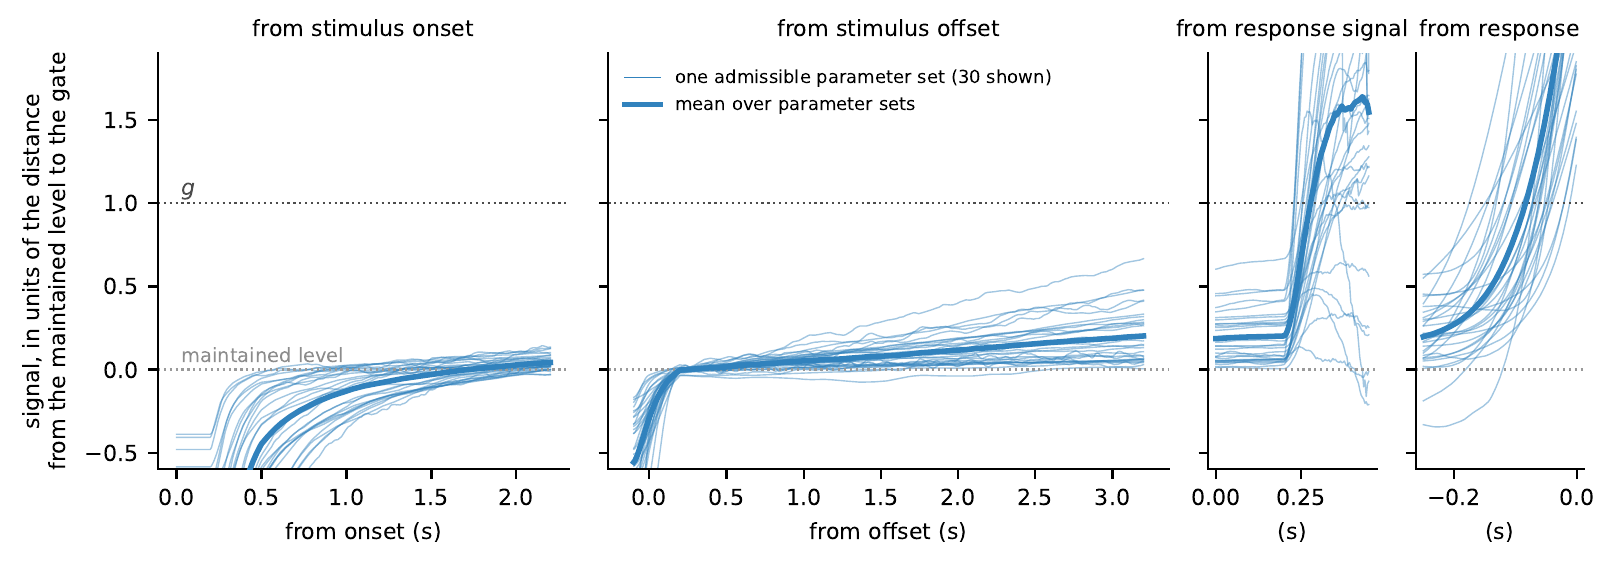
\includegraphics[width=\linewidth]{figures/fig01.png}\end{center}

\begin{center}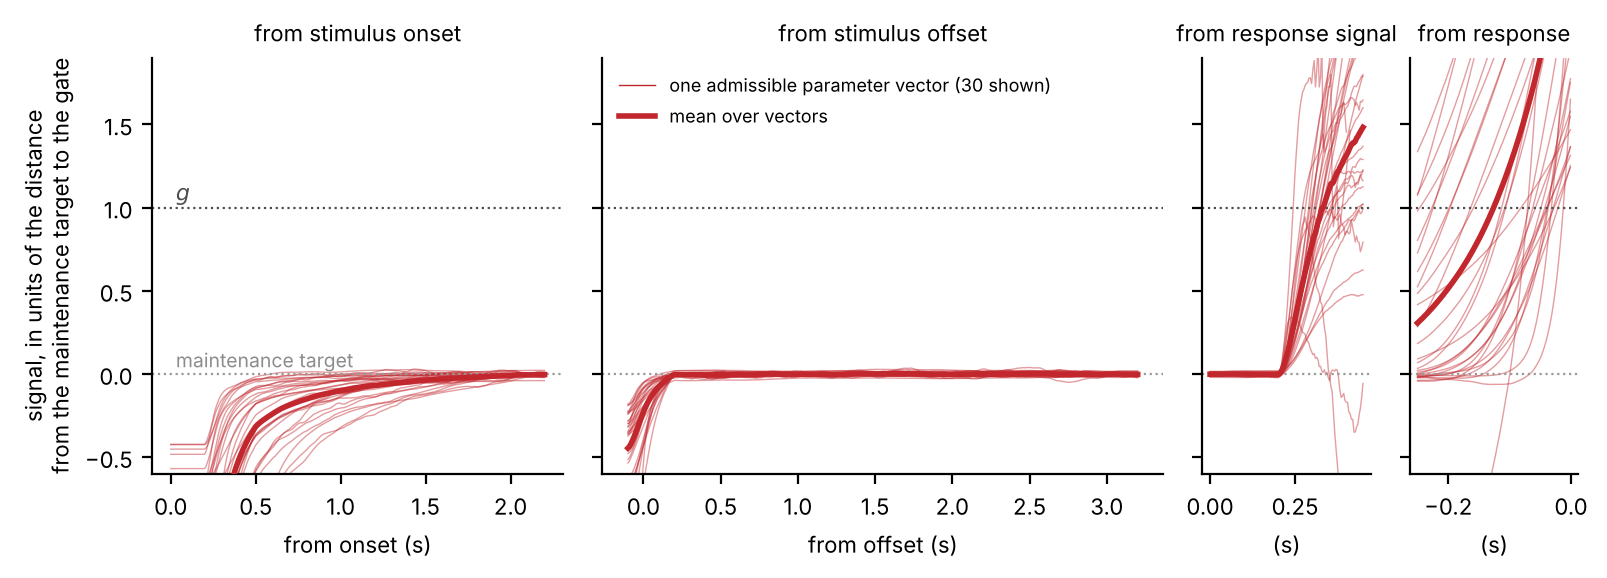
\includegraphics[width=\linewidth]{figures/fig02.png}\end{center}

\new{Fig 1. Simulated dynamics under the two candidate models.}  \new{Mean gated motor-preparatory signal at a representative admissible parameter vector --- the sampled draw closest to the coordinate-wise median of the parameters of the draws admissible in both models, with the ramp magnitude $\beta$ at the median of the values admissible under Model 2 (Materials and Methods),} \new{time-locked to the four trial events (stimulus onset, stimulus offset, response signal, response); each trial is censored at its own response.} \new{Each thin line is the mean over trials of one admissible parameter set, and the thick line the mean over parameter sets; thirty sets are shown, the same ones in both panels, so that the two differ in $\beta$ and in nothing else. The variability displayed is therefore variability across the parameter space rather than across trials at one setting, which is the variability every claim in the paper is about. The vertical axis is in units of each set's own distance from the maintained level to the gate, so that sets with different amplitudes are superimposable; 0 is the maintained level and 1 the gate.} \new{Color denotes motion coherence and line style denotes stimulus duration; dotted lines mark the internal threshold $\theta$ and the gate g. Top: Model 2 (maintained evidence-dependent state plus temporal preparation).} \new{Bottom: Model 1 (maintained evidence-dependent state only), at the same parameter vector with} $\beta =0$\new{. The two panels therefore differ in $\beta$ and in nothing else, which is the only term in which the architectures differ.} \new{The two models differ only during the delay period, where Model 2 climbs toward the gate as the response signal approaches and Model 1 does not. The panels show means across simulated trials: the clean separation between conditions visible here is a population-level regularity, not something any single trial exhibits on its own --- compare Fig 2B, one simulated trial.}

\begin{center}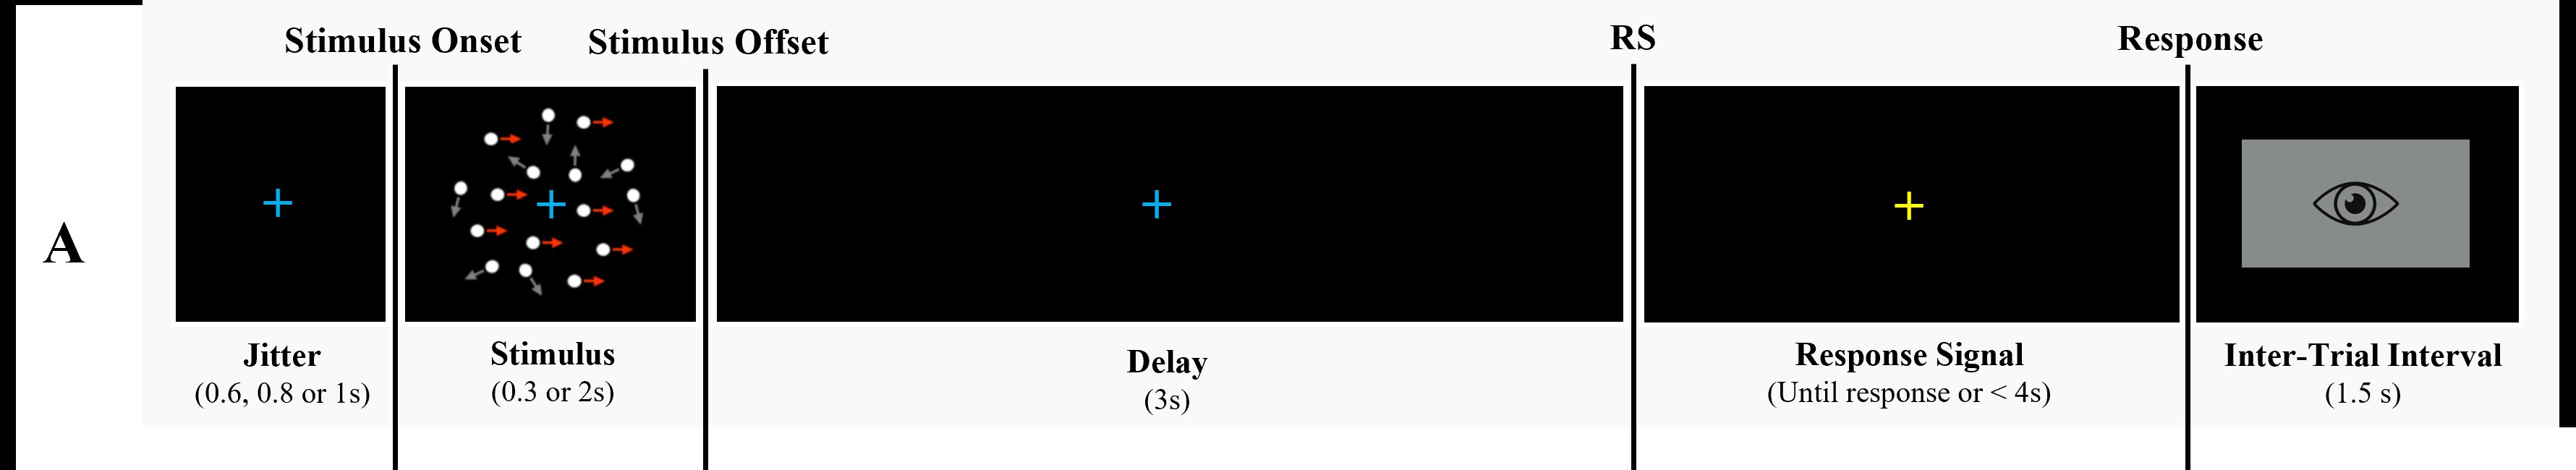
\includegraphics[width=\linewidth]{figures/fig03.png}\end{center}

\begin{center}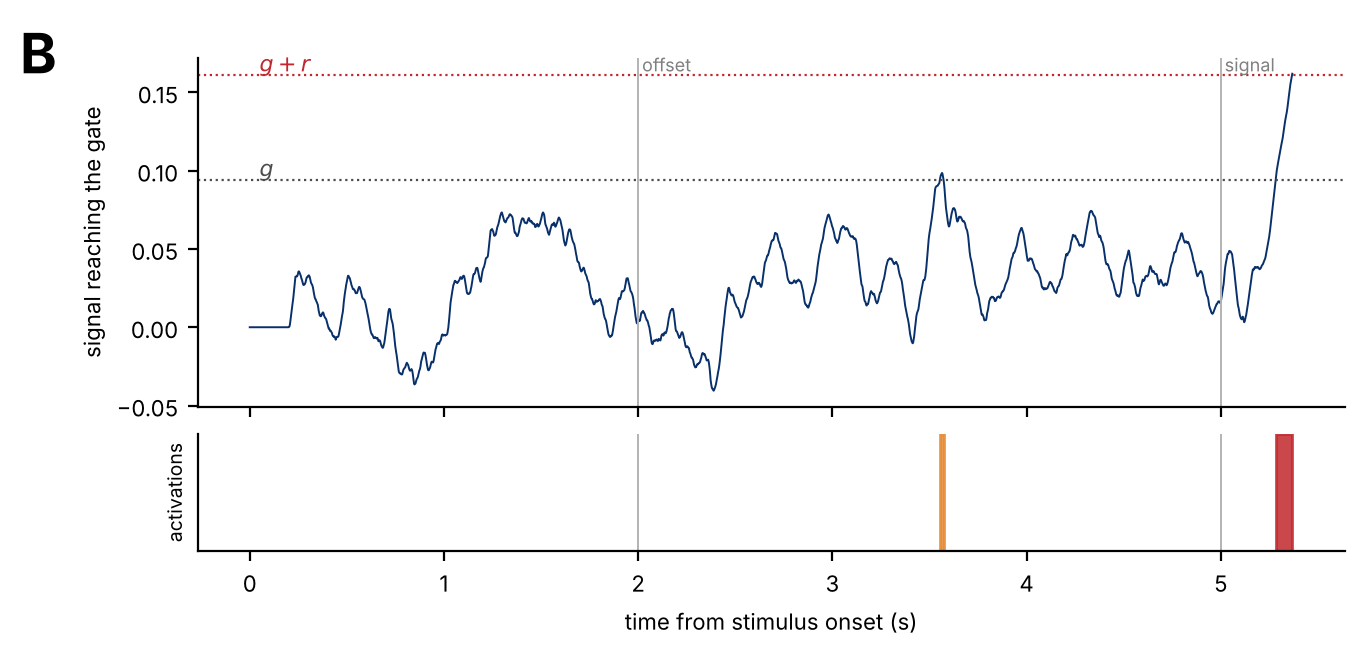
\includegraphics[width=\linewidth]{figures/fig04.png}\end{center}

\textbf{Fig 2. Experimental design and single-trial theoretical dynamics at the motor preparation and muscle activation levels}\textbf{.}  Panel A illustrates the time-course of a trial in our response signal (RS) variant of the random-dot motion task. See text for details.   Muscle activation begins when motor preparation exceeds gating inhibition (parameter \emph{g}). The response time (RT) corresponds to the latency between RS onset and the response. In the present study, it is decomposed into a pre-motor execution time (PMET) and a motor execution time (MET), based on the onset of muscle activation leading up to the response.   \new{Panel B shows one simulated trial from Model 2 at the representative admissible parameter vector of Fig 1}, the single-trial counterpart of the mean trajectories in Fig 1. Above, the gated signal reaching the response effector, with the gate g and the response criterion g+r; below, the activation intervals returned by the same detection procedure applied to the EMG data (see Materials and Methods), after merging intervals within 25 ms and discarding intervals with too few supra-threshold samples. Orange marks a partial muscle activation; red marks the activation that reaches the criterion and becomes the overt response.

\begin{center}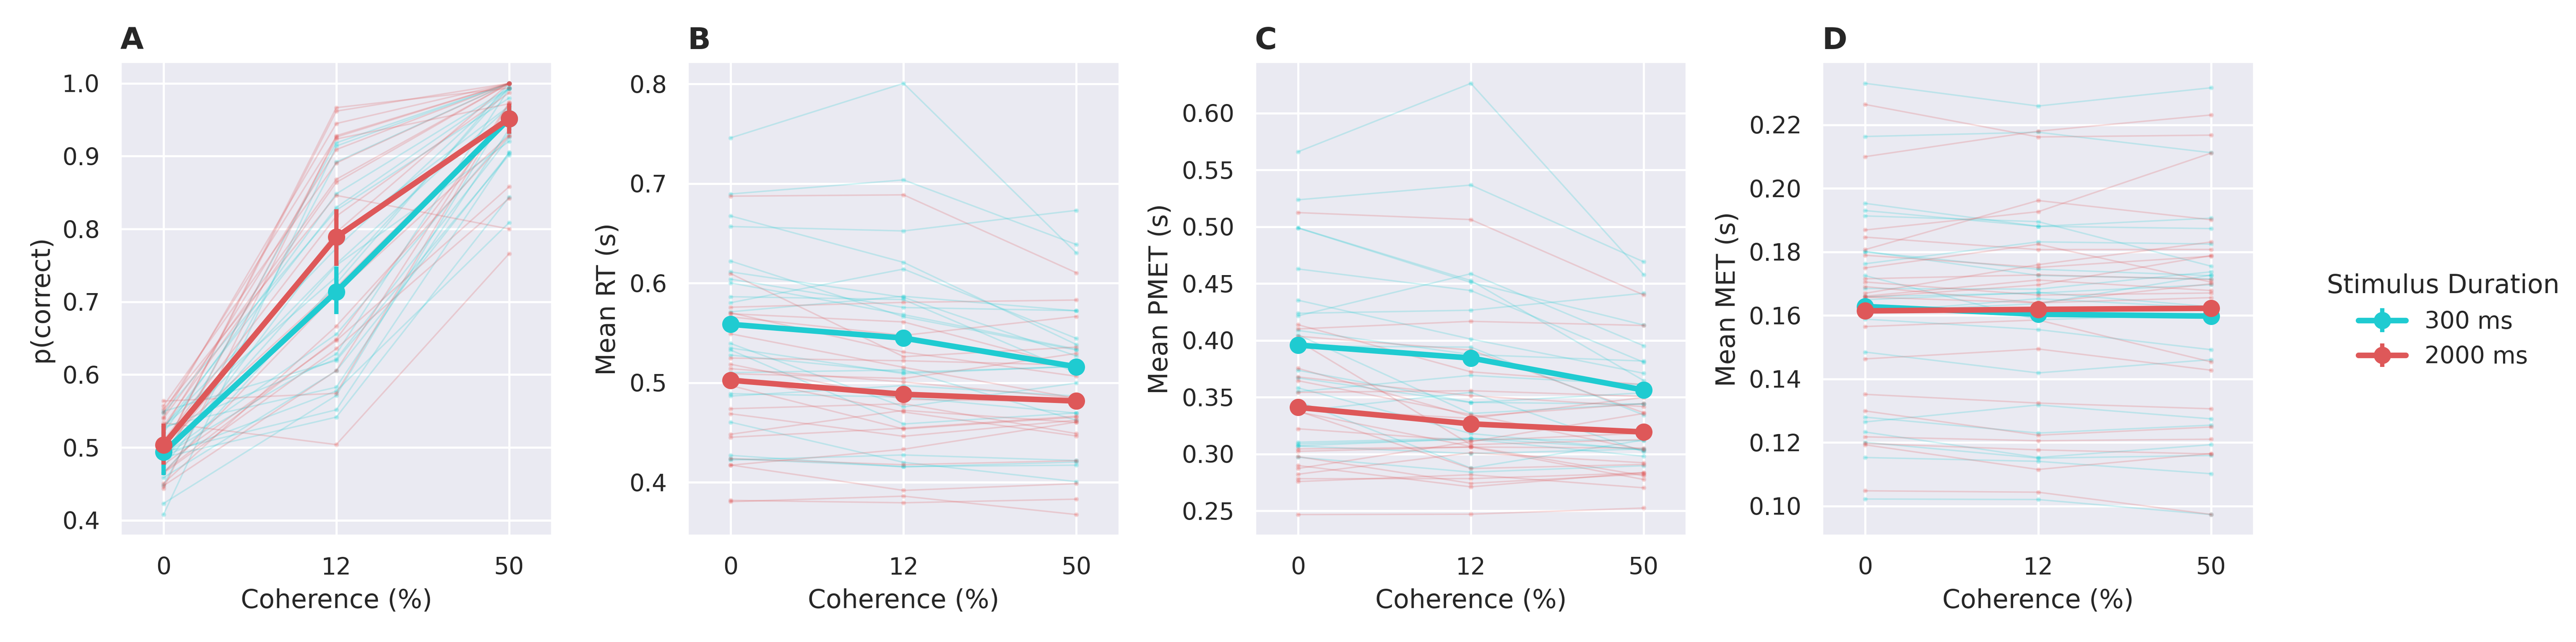
\includegraphics[width=\linewidth]{figures/fig05.png}\end{center}

Fig 3. Behavioral outcomes and response time fractionation based on the onset of muscle activation preceding the response. Panels A-D show, respectively, response accuracy, mean response time (RT), mean pre-motor execution time (PMET), and mean motor execution time (MET) as a function of motion coherence and duration. \new{Faint lines show individual participants.} \new{Error bars represent a within-subjects interval about the mean, computed on Cousineau--Morey-normalized values \parencite{moreyConfidenceIntervalsNormalized2008} in every panel: $\pm$1 within-subjects SEM for RT, PMET, and MET, and, for accuracy, a 95\% percentile bootstrap interval over the normalized values (10,000 resamples over participants, Morey-scaled), which is asymmetric where the data approach the [0, 1] bounds and for which a symmetric SEM would not be appropriate.}  s = seconds.

\begin{center}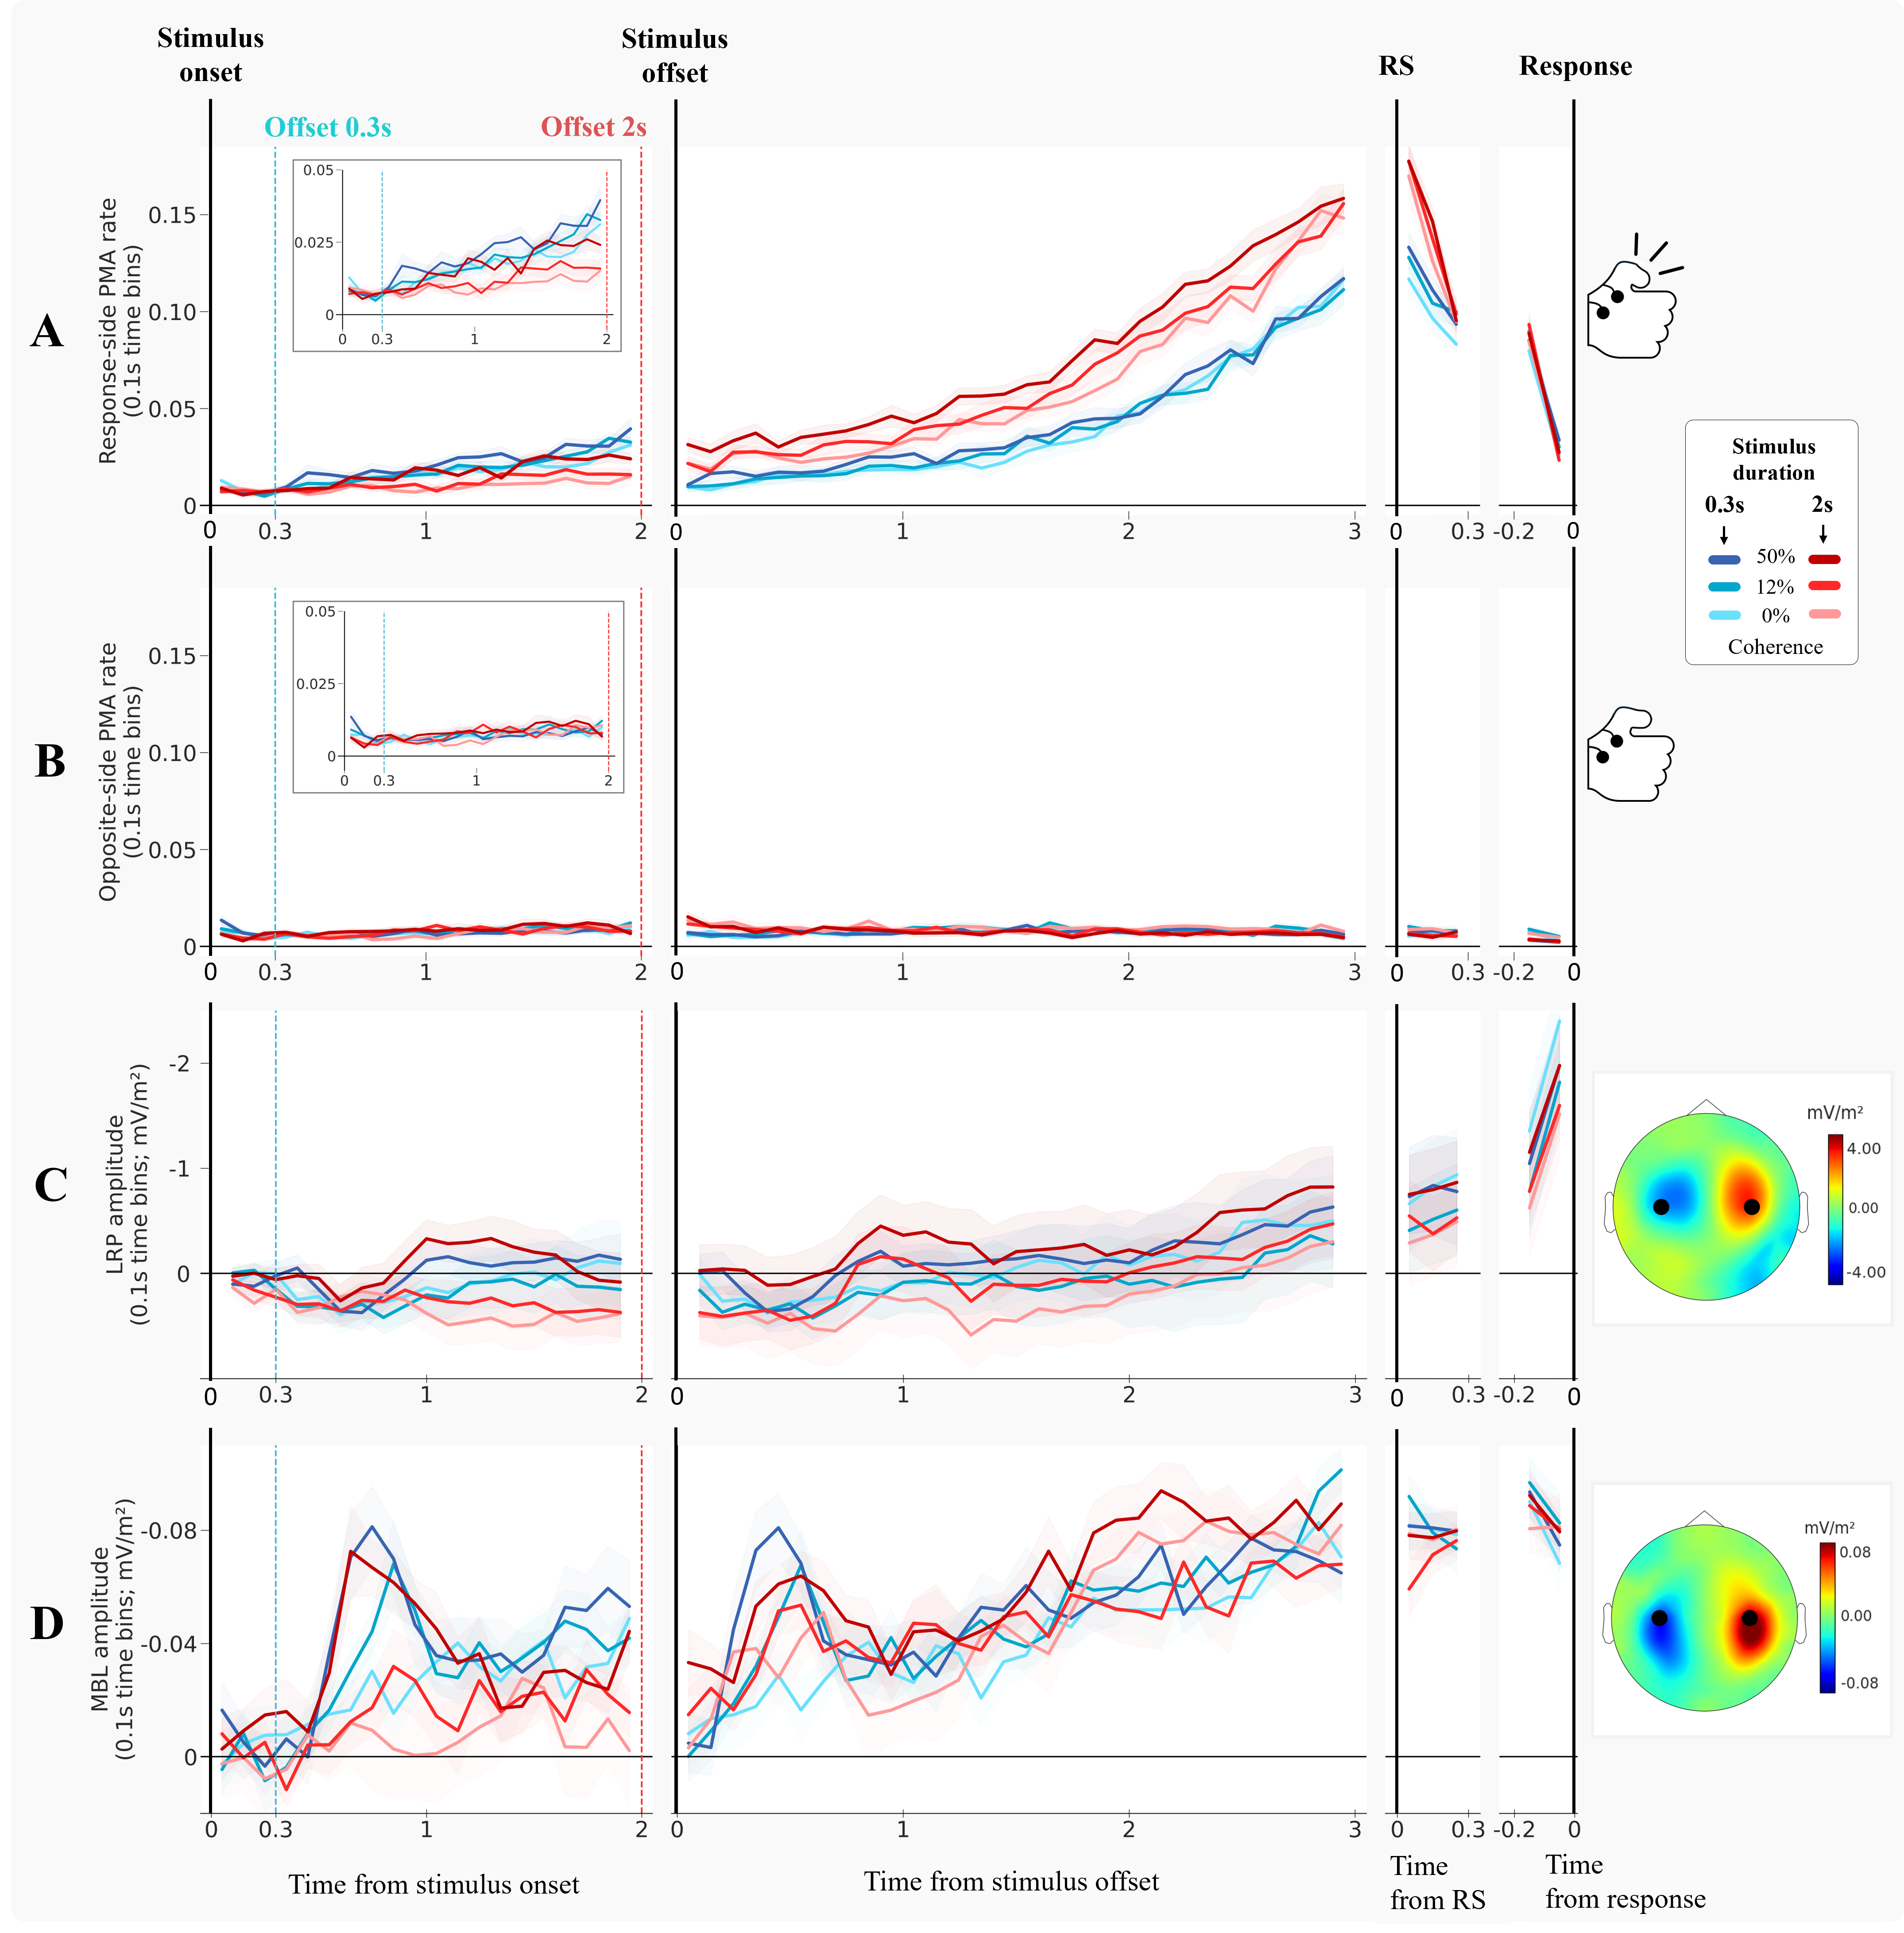
\includegraphics[width=\linewidth]{figures/fig06.png}\end{center}

\textbf{Fig 4. Rate of partial muscle activations and electroencephalographic measures of effector-selective motor preparation aligned to each trial event}\textbf{.}  A) Grand-average rate of partial muscle activations (PMAs) in the electromyographic channel of the responding effector as a function of motion coherence and duration. PMA rate was estimated as the mean number of PMAs per 0.1-s bin.  From left to right, subplots show PMA rate aligned to stimulus onset, stimulus offset, RS onset, and the response, respectively. These locking events are indicated by the black vertical lines. The inset in the leftmost subplot provides a zoomed view of the corresponding data. The grand-average rate of PMAs in the opposite electromyographic channel is shown in panel B. C) Grand-average lateralized readiness potential (LRP)  computed in 0.1 s bins, as a function of motion coherence and duration. The layout of the subplots matches that of panels A and B.  The y-axis is inverted such that upward deflections indicate stronger effector-selective motor preparation. The map on the right shows the grand-average scalp topography in the -0.2 to 0 s interval relative to the response, collapsed across experimental conditions. It was computed by subtracting the mean current source density amplitude for right-hand trials from that for left-hand trials. Black circles indicate the electrode sites used to compute the LRP (C3 and C4). D) Grand-average mu--beta-band spectral amplitude lateralization (MBL), computed in 0.1 s bins, as a function of motion coherence and duration. The y-axis is also inverted such that upward deflections indicate stronger effector-selective motor preparation.  The layout of the subplots matches that of the other panels.  The map on the right shows the grand-average scalp topography in the -0.2 to 0 s interval relative to the response, collapsed across experimental conditions. It was computed by subtracting the mean mu--beta-band spectral amplitude for right-hand trials from that for left-hand trials. For all panels, shaded areas represent $\pm$1 within-subjects standard error of the mean, computed using the method proposed by \textcite{moreyConfidenceIntervalsNormalized2008}.  s = seconds; mV/m\textsuperscript{2} = millivolts per square meter.


\section{Tables}

\textbf{Table 1.} \textbf{S}\textbf{ignificant effects from the ANOVAs on}  \textbf{response} \textbf{accuracy, mean} \textbf{response time (}\textbf{RT}\textbf{)}\textbf{,} \textbf{mean pre-motor execution time (PMET), and mean motor execution time (}\textbf{MET}\textbf{)}\textbf{.}

\begin{center}\small
\resizebox{\ifdim\width>\linewidth\linewidth\else\width\fi}{!}{%
\begin{tabular}{llll}
\toprule
Dependent variable &  & Significant effects & \emph{p}-value \\ \midrule
Accuracy &  & duration & \emph{p}  < .001 \\
 &  & coherence & \emph{p}  < .001 \\
 &  & duration $\times$ coherence & \emph{p}  < .001 \\
 &  &  &  \\
Mean RT &  & duration & \emph{p}  < .001 \\
 &  & coherence & \emph{p}  < .001 \\
 &  & duration $\times$ coherence & \emph{p} =  .016 \\
 &  &  &  \\
Mean PMET &  & duration & \emph{p}  < .001 \\
 &  & coherence & \emph{p}  < .001 \\
 &  & duration $\times$ coherence & \emph{p}  =  .035 \\
 &  &  &  \\
Mean MET &  & -- & -- \\
\bottomrule
\end{tabular}
}
\end{center}
\emph{Note}. Full ANOVA results, including effect sizes, are reported in Table S1.

\textbf{Table 2}\textbf{.} \textbf{Significant effects from the ANOVAs on partial muscle activation (PMA)} \textbf{rate} \textbf{in the electromy}\textbf{ographic channel of} \textbf{the responding effector}\textbf{,} \textbf{mu--beta-band spectral amplitude lateralization (MBL)}\textbf{, and lateralized readiness potential (LRP) amplitude} \textbf{across}  \textbf{task} \textbf{period}\textbf{s}\textbf{.}

\begin{center}\small
\resizebox{\ifdim\width>\linewidth\linewidth\else\width\fi}{!}{%
\begin{tabular}{llllllllll}
\toprule
Dependent variable & Significant effects &  & \multicolumn{7}{c}{Period} \\ \midrule
 &  &  &  &  &  &  &  &  &  \\
 &  &  & Stimulus &  & Delay &  & RS &  & Response \\
PMA rate & duration &  & \emph{p} = .001 &  & \emph{p} < .001 &  & \emph{p} < .001 &  & \new{p = .012} \\
 & coherence &  & \emph{p} = .021 &  & \new{\emph{p = .045}} &  & -- &  & -- \\
 & time (linear) &  & p < .001 &  & p < .001 &  & \emph{p} < .001 &  & \new{n/a$\dagger$} \\
 & duration $\times$ coherence &  & -- &  & \new{\emph{p = .042}} &  & -- &  & -- \\
 & duration $\times$ time (linear) &  & \new{p = .006} &  & \new{p = .002} &  & \emph{p} = .015 &  & \new{n/a$\dagger$} \\
 & coherence $\times$ time (linear) &  & \new{p = .007} &  & -- &  & -- &  & -- \\
 & time (quadratic) &  & -- &  & p < .001 &  & -- \textparagraph{} &  & -- \textparagraph{} \\
MBL amplitude & time (linear) &  & \new{p = .003} &  & \new{p = .014} &  & -- &  & \emph{p}  = .003 \\
 & coherence $\times$ time (linear) &  & \new{-- $\ddagger$} &  & -- &  & -- &  & -- \\
 & \new{duration $\times$ time (linear)} &  & \new{p = .046 \S{}} &  & \new{--} &  & \new{--} &  & \new{--} \\
 & time (quadratic) &  & p = .007 &  & -- &  & -- \textparagraph{} &  & -- \textparagraph{} \\
LRP amplitude & time (linear) &  & -- &  & \new{p = .001} &  & \emph{p} = .001 &  & \emph{p} < .001 \\
LRP amplitude & duration $\times$ time (quadratic) &  & p = .014 &  & -- &  & -- \textparagraph{} &  & -- \textparagraph{} \\
\bottomrule
\end{tabular}
}
\end{center}
\new{Note. Entries indicate p-values for significant effects. For stimulus- and delay-period time-bin effects, significance is based on the linear-trend or quadratic contrast rather than on the omnibus ANOVA (Methods). RS and response periods are unaffected (RS has only two time bins, where the omnibus and trend tests coincide exactly; the response period is analyzed on a single bin, so no trend decomposition applies there). Full ANOVA results, including effect sizes, are reported in Tables S2--S3. Time refers to the time-bin factor. RS = response signal. The response period is analyzed on its single informative bin, so its time-bin main effect and time-bin interactions (marked n/a$\dagger$) are not separate tests (Methods). $\ddagger$ Significant on the omnibus test (p < .001) but not as a full-window linear trend (p = .596): the effect is confined to the first half of the stimulus period and absent in the second half (Results; Table S4). \S{} Not significant on the omnibus test (p = .136) but significant as a linear trend (p = .046); reported here for consistency with the trend criterion used throughout this table. \textparagraph{} No quadratic contrast exists for RS or Response (only two time bins).}


\section{Appendix. The rate of partial muscle activations}

\new{This appendix derives the instantaneous rate at which the maintained motor-preparatory signal crosses the gate upward --- a partial muscle activation --- and the structural properties of that rate which the Results test. It contains no numerical evaluation: every quantity computed over the sampled parameter space is reported in Results, beside the data it is compared with.}

\new{\textbf{\emph{Setup and notation}}}

\new{Notation follows Theory (Materials and Methods) and Table A1;} $\varphi$ \new{and} $\Phi$ \new{are the standard normal density and distribution function. Fix a trial that has entered maintenance at time} ${\tau }_{0}$ \new{with selected response} ${s}_{\mathrm{resp}}$ \new{and maintained level} $m$ \new{(Equation (4)), and write} $\rho :=t-{\tau }_{0}$ \new{for elapsed maintenance time. For} $t\ge {\tau }_{0}$ \new{write} $y\left(t\right)=m+H\left(t\right)$\new{, so that} $H$ \new{is the fluctuation of the motor-preparatory signal about its target, with} $H\left({\tau }_{0}\right)=0$\new{. By Equations (5) and (6),} $H$ \new{is the output of the first-order filter driven by the Ornstein--Uhlenbeck maintenance noise:}

\begin{equation}
\dd \varepsilon \left(t\right)=-\kappa \varepsilon \left(t\right)\, \dd t+{\sigma }_{\varepsilon }\, \dd {W}_{\varepsilon }\left(t\right), \dd H\left(t\right)=\lambda \left(\varepsilon \left(t\right)-H\left(t\right)\right)\, \dd t, \varepsilon \left({\tau }_{0}\right)=H\left({\tau }_{0}\right)=0
\tag{11}
\end{equation}

\new{with} ${\sigma }_{\varepsilon }={\mathrm{SD}}_{\varepsilon }\sqrt{2\kappa }$\new{, so that the stationary standard deviation of} $\varepsilon$ \new{is} ${\mathrm{SD}}_{\varepsilon }$ \new{whatever the value of} $\kappa$\new{, and the two are sampled independently in Table A1. Because} $\varepsilon$ \new{is symmetric and independent of the sign of the response,} ${s}_{\mathrm{resp}}H$ \new{has the same law as} $H$\new{. Writing} $\delta :={t}_{\mathrm{RS}}-{t}_{\mathrm{offset}}$ \new{for the length of the preparation window and} $d\left(t\right)$ \new{for the distance from the maintained level to the gate,}

\begin{equation}
d\left(t\right)=g-\left|m\right|-\frac{\beta }{\delta }{\left(t-{t}_{\mathrm{offset}}\right)}^{+}
\tag{12}
\end{equation}

\new{(the second term present only under temporal preparation, so that} $\beta =0$ \new{under Model 1), a partial activation on the selected channel begins exactly when} ${s}_{\mathrm{resp}}H$ \new{crosses} $d\left(t\right)$ \new{upward. The ramp therefore approaches the gate at the constant speed} $\beta /\delta$\new{. The non-selected channel activates when} ${s}_{\mathrm{resp}}H$ \new{falls below the corresponding distance on the far side, which is several fluctuation standard deviations further away over the whole admissible space; the model predicts that channel to be silent, as it is observed to be, and it is not considered further.}

\new{\textbf{Table A1.}} \old{Variables and parameters of the extended evidence-accumulation model for delayed reports.}

\begin{center}\small
\begin{tabular}{>{\raggedright\arraybackslash}p{0.095\linewidth}>{\raggedright\arraybackslash}p{0.541\linewidth}>{\raggedright\arraybackslash}p{0.294\linewidth}}
\toprule
\old{Symbol} & \old{Description} & \old{Value or range used in simulations (if applicable)} \\ \midrule
\old{\emph{t}} & \old{Time measured from motion-stimulus onset} & \old{---} \\
\old{\emph{x(t)}} & \old{Accumulated} \old{motion} \old{evidence} & \old{See} \old{Eq. (1)} \\
\old{\emph{L}}\old{\textsubscript{m}\textsubscript{o}\textsubscript{t}\textsubscript{i}\textsubscript{o}\textsubscript{n}} & \old{Motion-}\old{evidence}  \old{encoding}  \old{latency} & \old{0.200 s} \\
\old{\emph{s}} & \old{Motion direction} & \old{$-$1 or +1} \\
\old{\emph{c}} & \old{Motion} \old{coherence} & \old{0, 0.12, or 0.50} \\
\old{\emph{k}} & \old{Scaling of motion coherence into the mean rate of motion-evidence accumulation} & \new{0.5--2.0 (log-uniform); \textcite{dendauwGatedCascadeDiffusion2024} estimate 1.183} \\
\old{\emph{$\sigma$}}\old{\textsubscript{x}} & \old{Diffusion coefficient of motion-}\old{evidence} \old{accumulation} & \old{0.100} \\
\old{\emph{y(t)}} & \old{Filtered}  \old{motor-preparatory} \old{state} & \old{See}  \old{Eqs}\old{. (2), (6), and (9}\old{)} \\
\old{\emph{$\lambda$}} & \old{Gain of the low-pass filter relating decision-related input to motor preparation} & \new{10--50 s\textsuperscript{-1} (log-uniform); \textcite{dendauwGatedCascadeDiffusion2024} estimate 21.471} \\
\old{z}\old{\emph{\textsubscript{L}}}\old{(}\old{\emph{t}}\old{),} \old{z}\old{\emph{\textsubscript{R}}}\old{(}\old{\emph{t}}\old{)} & \old{Neural drives to the left and right response agonists} & \old{See} \old{Eq. (3)} \\
\old{\emph{g}} & \old{Level} \old{of} \old{gating} \old{inhibition} & \new{0.050--0.200} \\
\old{\emph{r}} & \old{Response criterion applied to the neural drive} & \new{0.010--0.200 (log-uniform)} \\
\old{\emph{L}}\old{\textsubscript{m}\textsubscript{o}\textsubscript{t}\textsubscript{o}\textsubscript{r}} & \old{Residual motor latency between response triggering and the overt response} & \new{0.093 s (fixed; Dendauw et al. 2024)} \\
\old{\emph{D}} & \old{Motion duration} & \old{0.300 or 2.000 s} \\
\old{\emph{$\theta$}} & \old{Internal motor-preparation threshold triggering maintenance} & \old{\emph{$\theta$/g}}  \old{sampled}  \old{from} \old{0.25--0.90} \\
\old{\emph{$\tau$}} & \old{Maintenance-}\old{onset} \old{time} & \old{Trial-}\old{dependent} \\
\old{\emph{m}} & \old{Maintenance} \old{target} & \old{See} \old{Eq. (4)} \\
\old{\emph{s}}\old{\textsubscript{r}\textsubscript{e}\textsubscript{s}\textsubscript{p}} & \old{Selected}  \old{response} \old{direction} & \old{$-$1:} \old{left}\old{; +1: right} \\
\old{\emph{$\varepsilon$(t)}} & \old{Stochastic fluctuations around the maintenance target} & \old{See} \old{Eq. (5)} \\
\new{\emph{$\kappa$}} & \old{Mean-reversion rate of maintenance fluctuations} & \new{0.20--30.0 s\textsuperscript{-1} (log-uniform)} \\
\old{\emph{$\sigma$}}\old{\textsubscript{$\varepsilon$}} & \old{Diffusion coefficient of maintenance fluctuations} & \new{=} ${\mathrm{SD}}_{\varepsilon }\sqrt{2\kappa }$\new{, with} ${\mathrm{SD}}_{\varepsilon }$ \new{0.003--0.060 (log-uniform)} \\
\old{\emph{t}}\old{\textsubscript{offset}} & \old{Time at which stimulus offset becomes internally available as a temporal reference} & \old{\emph{D}} \old{+} \old{\emph{L}}\old{\textsubscript{motion}} \\
\old{\emph{L}}\old{\textsubscript{RS}} & \old{RS-}\old{evidence}  \old{encoding}  \old{latency} & \old{0.200 s} \\
\old{\emph{t}}\old{\textsubscript{RS}} & \old{Time at which RS evidence becomes available to the accumulation process} & \old{\emph{D}} \old{+ 3 +} \old{\emph{L}}\old{\textsubscript{RS}} \\
\old{\emph{$\beta$}} & \old{Maximum additive contribution of temporal preparation to the motor-preparatory signal reaching the downstream gate} & \new{Model 1: 0; Model 2: 0.0015--0.100 (log-uniform)} \\
\old{\emph{q(t)}} & \old{Accumulated evidence that the RS is present} & \old{See} \old{Eq. (8}\old{)} \\
\old{\emph{$\mu$}}\old{\textsubscript{RS}} & \old{Mean rate of RS-evidence accumulation} & \old{0.30--1.50} \\
\old{\emph{$\sigma$}}\old{\emph{\textsubscript{q}}} & \old{Diffusion coefficient of RS-}\old{evidence} \old{accumulation} & \new{0.03--0.30 (log-uniform)} \\
\bottomrule
\end{tabular}
\end{center}
\new{Note.} \new{The values and ranges in this table come from the design of the experiment, from published estimates, or from the structure of the model itself;} \new{none is derived from these data, since a range drawn around a value estimated from the data cannot test whether a prediction survives away from that value.} \new{$\sigma$x is not an empirical quantity at all: the model is exactly invariant under a joint rescaling of every amplitude it contains (k, $\sigma$x, $\theta$, g, r, SD$\varepsilon$, $\mu$RS, $\sigma$q and $\beta$), so one of them must be fixed to set the units, and the remaining amplitudes are in effect expressed in units of $\sigma$x. k and $\lambda$ were estimated by \textcite{dendauwGatedCascadeDiffusion2024} in an immediate-report task; because constants inherited from immediate report are not guaranteed to transfer to delayed report, both were sampled over roughly a factor of two either side of those estimates} \new{rather than fixed at them --- as was the response criterion r, for the same reason. The residual motor latency Lmotor is the one exception: it is fixed at Dendauw et al.'s 0.093 s, on the ground that a peripheral electromechanical delay between muscle activation and the overt response has better reason to transfer between tasks than a decision-related constant does.} \new{The upper end of $\lambda$ follows from reading 1/$\lambda$ as the time constant of the filter relating decision-related input to motor preparation: the sampled range corresponds to time constants between 100 and 20 ms, whereas} $\lambda =100 {\mathrm{s}}^{-1}$ \new{would imply 10 ms, faster than plausible neuromuscular filtering. That bound also bears on the ceiling argument of Results (Delay-locked), which weakens as $\lambda$ grows, and is stated here so that it is visible as a modeling commitment rather than a convenience.} \new{$\sigma$q was likewise sampled rather than fixed, over a factor of three either side of parity with $\sigma$x, on the structural analogy between the two accumulators; it is weakly identified by behavior, so fixing it would amount to an unexamined assumption. $\kappa$ is not constrained by any prior study in this paradigm and was sampled over more than two orders of magnitude, from a maintenance fluctuation whose correlation time exceeds the entire delay} $\left(1/\kappa =5 \mathrm{s}\right)$ \new{to one that decorrelates within a single analysis bin (33 ms); the range is deliberately generous, and generous in the direction that favors Model 1, whose only route to a delay-period rate still rising at the end of the delay is a small $\kappa$. The motion- and RS-evidence encoding latencies Lmotion and LRS were both fixed at 0.200 s as a simplifying choice for the simulations. The} $\theta /g$\new{, rather than $\theta$ itself, was sampled to ensure} $\theta <g$\new{, which the architecture requires.} \new{For the maintenance-noise process, the stationary standard deviation SD$\varepsilon$ is sampled rather than $\sigma$$\varepsilon$, so that fluctuation amplitude varies independently of $\kappa$; it is sampled directly rather than through any quantity derived from it, so that the sampling law over the space is the one the table states.} \new{The remaining ranges --- g, $\theta$/g, SD$\varepsilon$, $\beta$ and $\mu$RS --- are deliberately wider than the region the task-admissibility screen accepts, so that what constrains the space evaluated is that screen, whose criteria are taken from the design of the experiment, rather than the choice of endpoints. RS: response signal.}

\new{\textbf{\emph{The maintained fluctuation}}}

\new{Solving the two equations of (11) in sequence gives}

\begin{equation}
\varepsilon \left({\tau }_{0}+\rho \right)={\sigma }_{\varepsilon }\int_{0}^{\rho } {e}^{-\kappa \left(\rho -p\right)}\, \dd {W}_{\varepsilon }\left(p\right), H\left({\tau }_{0}+\rho \right)=\lambda \int_{0}^{\rho } {e}^{-\lambda \left(\rho -q\right)}\varepsilon \left({\tau }_{0}+q\right)\, \dd q
\tag{13}
\end{equation}

\new{The Ornstein--Uhlenbeck process admits a continuous modification, and} $H$ \new{is then a Riemann integral of a continuous function, so almost surely} $H$ \new{is continuously differentiable --- which is what the crossing formula below requires and what an unfiltered diffusion would not provide. Substituting the first equation of (13) into the second and exchanging the order of integration --- permissible because the integrand is bounded on the compact} $\{0\le p\le q\le \rho \}$ \new{--- leaves the inner integral} $\int_{p}^{\rho } \lambda {e}^{-\lambda \left(\rho -q\right)}{e}^{-\kappa \left(q-p\right)}\, \dd q$\new{. Hence} $H$ \new{is a Wiener integral against the impulse response of the two filters in series,}

\begin{equation}
H\left({\tau }_{0}+\rho \right)=\int_{0}^{\rho } K\left(\rho -p\right)\, \dd {W}_{\varepsilon }\left(p\right), K\left(v\right)=\frac{\lambda {\sigma }_{\varepsilon }}{\lambda -\kappa }\left({e}^{-\kappa v}-{e}^{-\lambda v}\right)
\tag{14}
\end{equation}

\new{and is therefore a centred Gaussian process.} $K\left(0\right)=0$\new{, which is the analytic form the differentiability takes, and} ${K}^{'}\left(0\right)=\lambda {\sigma }_{\varepsilon }$\new{.}

\new{Differentiating (14) under the integral, and using} $K\left(0\right)=0$ \new{to kill the boundary term, gives} $\dot{H}\left({\tau }_{0}+\rho \right)=\int_{0}^{\rho } {K}^{'}\left(\rho -p\right)\, \dd {W}_{\varepsilon }\left(p\right)$\new{. The It\^o isometry then gives the three second moments as integrals of the kernel,} $\Var H=\int_{0}^{\rho } {K}^{2}$\new{,} $\Var \dot{H}=\int_{0}^{\rho } {\left({K}^{'}\right)}^{2}$ \new{and} $\Cov \left(H,\dot{H}\right)=\int_{0}^{\rho } K{K}^{'}=1/2K{\left(\rho \right)}^{2}$\new{, the last of which is half the derivative of the first. Evaluating them,}

\begin{equation}
\Var H\left(\rho \right)=\frac{{\lambda }^{2}{\sigma }_{\varepsilon }^{2}}{{\left(\lambda -\kappa \right)}^{2}}\left[\frac{1-{e}^{-2\kappa \rho }}{2\kappa }-\frac{2\left(1-{e}^{-\left(\lambda +\kappa \right)\rho }\right)}{\lambda +\kappa }+\frac{1-{e}^{-2\lambda \rho }}{2\lambda }\right]
\tag{15}
\end{equation}

\begin{equation}
\Var \dot{H}\left(\rho \right)=\frac{{\lambda }^{2}{\sigma }_{\varepsilon }^{2}}{{\left(\lambda -\kappa \right)}^{2}}\left[\frac{\kappa \left(1-{e}^{-2\kappa \rho }\right)}{2}-\frac{2\kappa \lambda \left(1-{e}^{-\left(\lambda +\kappa \right)\rho }\right)}{\lambda +\kappa }+\frac{\lambda \left(1-{e}^{-2\lambda \rho }\right)}{2}\right]
\tag{16}
\end{equation}

\new{These hold when the two rates differ. When they coincide the cascade has a repeated pole: the basis} $\{{e}^{-\kappa v},{e}^{-\lambda v}\}$ \new{degenerates into} $\{{e}^{-\lambda v},v{e}^{-\lambda v}\}$\new{, and (14) to (16) are replaced by their limits at} $\kappa =\lambda$\new{, namely} $K\left(v\right)=\lambda {\sigma }_{\varepsilon }v{e}^{-\lambda v}$ \new{and, writing} $E={e}^{-2\lambda \rho }$\new{,}

\begin{equation}
\Var H\left(\rho \right)=\frac{{\sigma }_{\varepsilon }^{2}}{4\lambda }\left[1-E\left(1+2\lambda \rho +2{\lambda }^{2}{\rho }^{2}\right)\right], \Var \dot{H}\left(\rho \right)=\frac{\lambda {\sigma }_{\varepsilon }^{2}}{4}\left[1-E\left(1-2\lambda \rho +2{\lambda }^{2}{\rho }^{2}\right)\right]
\tag{17}
\end{equation}

\new{The two cases meet continuously:} $\kappa =\lambda$ \new{is a coincidence of the two rates, not a singularity of the process. It is also the one point in the space at which the model has no separation of timescales, the correlation time of the maintenance noise and the time constant of the motor filter being equal; the consequences are drawn where they arise, in A.5 and A.9.}

\new{As} $\rho \to \infty$ \new{both cases tend to the same stationary values, which will be written} ${\sigma }_{H}$ \new{and} ${\sigma }_{\dot{H}}$\new{:}

\begin{equation}
{\sigma }_{H}^{2}=\frac{\lambda \, {\mathrm{SD}}_{\varepsilon }^{2}}{\lambda +\kappa }, {\sigma }_{\dot{H}}^{2}=\frac{{\lambda }^{2}\kappa \, {\mathrm{SD}}_{\varepsilon }^{2}}{\lambda +\kappa }, \Cov \left(H,\dot{H}\right)\to 0, \omega :=\frac{{\sigma }_{\dot{H}}}{{\sigma }_{H}}=\sqrt{\lambda \kappa }
\tag{18}
\end{equation}

$\omega$ \new{is the characteristic frequency of the fluctuation. The preparation ramp is added outside the filter (Equation (7)), so it shifts the mean of the gate-facing signal and leaves all three moments untouched; (15) to (18) hold for both models. The relative departure of} $\Var H$ \new{from} ${\sigma }_{H}^{2}$ \new{one second into maintenance is of order} ${e}^{-2\kappa }$\new{, which is negligible at the top of the range of} $\kappa$ \new{in Table A1 and of order one at its bottom. The stationary forms are therefore used only where that condition is checked; wherever the value of} $\kappa$ \new{bears on a conclusion the moments are taken from (15) to (17) directly. That is the region most favorable to Model 1, and therefore the region a bound must not approximate away.}

\new{\textbf{\emph{The crossing rate}}}

\new{Let} $Z\left(t\right):={s}_{\mathrm{resp}}H\left(t\right)-d\left(t\right)$\new{, so that upcrossings of} $d$ \new{by} ${s}_{\mathrm{resp}}H$ \new{are upcrossings of zero by} $Z$\new{, and} $\dot{Z}=\dot{H}+\beta /\delta$\new{. Trajectories that reach the response criterion before the end of the delay are neglected; they are premature responses, excluded from the empirical analysis and held to a small fraction of trials by the admissibility screen. Since} $H$ \new{is almost surely continuously differentiable and} $\left(Z,\dot{Z}\right)$ \new{is jointly Gaussian and non-degenerate for} $\rho >0$\new{, the Kac--Rice formula gives the expected upcrossing rate \parencite[ch. 3]{azaisLevelSetsExtrema2009}:}

\begin{equation}
\nu \left(t\right)={p}_{Z\left(t\right)}\left(0\right)\, \mathrm{E}\left[\dot{Z}\left(t\right){1}_{\{\dot{Z}\left(t\right)>0\}} | Z\left(t\right)=0\right]
\tag{19}
\end{equation}

\new{No stationarity is assumed: the formula requires only continuous differentiability and non-degenerate one-dimensional marginals, both of which hold from the moment maintenance begins. Since} $H$ \new{is centred,} $Z\left(t\right)\sim \mathrm{N}\left(-d\left(t\right),\Var H\right)$ \new{and} ${p}_{Z\left(t\right)}\left(0\right)=\varphi \left(d\left(t\right)/\sqrt{\Var H}\right)/\sqrt{\Var H}$\new{. Because} $\left(Z,\dot{Z}\right)$ \new{is jointly Gaussian,} $\dot{Z}$ \new{given} $Z=0$ \new{is Gaussian with}

\begin{equation}
M\left(t\right)=\frac{\beta }{\delta }+\frac{\Cov \left(H,\dot{H}\right)}{\Var H}d\left(t\right), S\left(t\right)=\Var \dot{H}-\frac{\Cov {\left(H,\dot{H}\right)}^{2}}{\Var H}
\tag{20}
\end{equation}

\new{and for} $X\sim \mathrm{N}\left(M,S\right)$ \new{one has} $\mathrm{E}\left[X{1}_{\{X>0\}}\right]=M\Phi \left(M/\sqrt{S}\right)+\sqrt{S}\varphi \left(M/\sqrt{S}\right)$\new{. Substituting into (19) gives the rate in general form,}

\begin{equation}
\nu \left(t\right)=\frac{\varphi \left(d\left(t\right)/\sqrt{\Var H}\right)}{\sqrt{\Var H}}\left[M\left(t\right)\Phi \left(\frac{M\left(t\right)}{\sqrt{S\left(t\right)}}\right)+\sqrt{S\left(t\right)}\varphi \left(\frac{M\left(t\right)}{\sqrt{S\left(t\right)}}\right)\right]
\tag{21}
\end{equation}

\new{Once the transient has passed the covariance vanishes, so} $M=\beta /\delta$ \new{and} $S={\sigma }_{\dot{H}}^{2}$\new{. Writing} $a\left(t\right):=d\left(t\right)/{\sigma }_{H}$ \new{for the standardized distance from the maintained level to the gate --- the one abbreviation kept, because it is the quantity every result below turns on --- (21) becomes}

\begin{equation}
\nu \left(t\right)=\varphi \left(a\left(t\right)\right)\left[\frac{\beta }{\delta {\sigma }_{H}}\Phi \left(\frac{\beta }{\delta {\sigma }_{\dot{H}}}\right)+\omega \varphi \left(\frac{\beta }{\delta {\sigma }_{\dot{H}}}\right)\right]
\tag{22}
\end{equation}

\new{the expression used in Results (Delay-locked). The bracket does not depend on the distance to the gate, and the ramp enters it only through} $\beta /\delta$\new{, the speed at which temporal preparation carries the signal toward the gate.}

\new{Corollary A.1 (the ceiling on Model 1's delay-period rate, and when it applies). Setting} $\beta =0$ \new{in (22) --- Model 1 --- gives the classical Rice formula,}

\begin{equation}
\nu =\frac{\omega }{2\pi }{e}^{-{a}^{2}/2}
\tag{23}
\end{equation}

\new{whose maximum over the standardized distance is} $\omega /2\pi =\sqrt{\lambda \kappa }/2\pi$\new{, attained when the gate sits at the maintained level. That bound holds only once the fluctuation is stationary. Before then, setting} $\beta =0$ \new{and} $d=0$ \new{in (21) gives} $M=0$ \new{and the exact ceiling}

\begin{equation}
\frac{1}{2\pi }\sqrt{\frac{\Var \dot{H}}{\Var H}-\frac{\Cov {\left(H,\dot{H}\right)}^{2}}{{\left(\Var H\right)}^{2}}}
\tag{24}
\end{equation}

\new{which exceeds} $\omega /2\pi$ \new{while the variance is still filling in, and diverges as} $\rho \to 0$\new{: at the very start of maintenance the fluctuation is smooth but its variance is small, so a gate placed at the maintained level is crossed very often. Non-stationarity therefore RAISES the ceiling rather than lowering it, and the covariance term subtracted in (24) offsets only a small part of that. The bound used in Results is (24), evaluated in the analyzed window. $\square$}

\new{Corollary A.2 (the log-rate slope). Under Model 2 the barrier moves at constant speed, so by (12) the standardized distance falls linearly,} $a\left(\tau \right)=a\left({\tau }_{0}\right)-\beta \tau /\left(\delta {\sigma }_{H}\right)$\new{. Taking logarithms in (22), the bracket is constant in} $\tau$ \new{and} $\ln \varphi \left(a\right)=-{a}^{2}/2-\ln \sqrt{2\pi }$\new{, so}

\begin{equation}
\frac{\dd \left(\ln \nu \right)}{\dd \tau }=\frac{\beta }{\delta {\sigma }_{H}}a\left(\tau \right), \frac{{\dd }^{2}\left(\ln \nu \right)}{\dd {\tau }^{2}}=-{\left(\frac{\beta }{\delta {\sigma }_{H}}\right)}^{2}
\tag{25}
\end{equation}

\new{The log rate rises at a rate proportional to the current standardized distance to the gate. Its curvature is negative, and constant in time --- the log rate is exactly a downward parabola --- with the same value in all six conditions, since} $\beta$\new{,} $\delta$ \new{and} ${\sigma }_{H}$ \new{are properties of the participant and not of the condition. A cell with a higher rate has a smaller standardized distance and so a shallower predicted log-rate slope. $\square$}

\new{Proposition A.3 (saturation and the coherence $\times$ duration interaction). The model predicts the effect of coherence on the delay-period rate to be smaller, not larger, after a long stimulus. Proof. The maintained TARGET is capped pathwise at} $\theta$\new{: a trial that reaches the threshold has its target pinned there for the rest of the delay, though its signal continues to fluctuate about that target. On such a trial the distance} $d$ \new{entering (21) is} $g-\theta$ \new{less the ramp, the same in every condition, and the law of} $H$ \new{does not depend on coherence either, so the rate is coherence-independent. Writing} $F\left(D,c\right)$ \new{for the fraction of trials at duration} $D$ \new{and coherence} $c$ \new{whose target has reached} $\theta$\new{, the coherence levels therefore converge on a common value as} $F\left(D,c\right)\to 1$\new{, and a longer stimulus raises} $F$ \new{at every coherence, moving every cell closer to it.}

\new{The argument is a limit argument, and the prediction holds only as the limit is approached. It requires the LOWEST-coherence long-duration cell to be near the cap: the effect is a difference between coherences, and the cap can shrink that difference only once both of its terms are capped. Where that fails the prediction reverses, for the converse reason: below the cap the target is free, its mean grows about as} $kc\left(t-1/\lambda \right)$\new{, and its coherence derivative} $k\left(t-1/\lambda \right)$ \new{grows with duration. Saturation is what turns that growth into a shrinkage. The condition cannot be enforced through accuracy, because the contrast is taken against the zero-coherence cell, whose accuracy is one half by symmetry at every parameter setting.}

\new{A second channel works in the same direction and is not covered by the argument above. The delay window is timed from stimulus offset, not from the crossing of} $\theta$\new{, and the crossing occurs earlier at higher coherence. Capped trials at high coherence have therefore been in maintenance longer when the window opens, their variance has filled in further, and their rate is correspondingly higher --- a residual coherence effect among capped trials, larger after the long stimulus than after the short one. It vanishes once the fluctuation is stationary well before the window opens, and so bites only at small} $\kappa$\new{, which is the regime in which Model 1 can produce any ramp at all. Its size, and the frequency with which either failure occurs over the admissible space, are reported in Results (Delay-locked). $\square$}

\new{Remark A.4. Corollary A.2 and Proposition A.3 pull in opposite directions on the coherence dependence of the delay-period rate, and are consistent. A.3 concerns the rate itself, whose coherence dependence saturates; A.2 concerns the slope of its logarithm, which remains coherence-dependent --- shallower where the rate is higher --- precisely because the distance to the gate is smaller there. A residual coherence dependence of the log-rate slope is a signature of saturated maintenance, not of continued evidence accumulation.}

\new{Corollary A.5 (Model 1 cannot ramp and activate at the same rate). Under Model 1 any delay-period ramp exists only by virtue of the non-stationarity of} $H$\new{, and it is traded off against the rate itself, the trade-off being carried by the standardized distance. Proof. Maintenance begins with the filtered signal exactly at its target and the Ornstein--Uhlenbeck input at its own mean, so} $H\left({\tau }_{0}\right)=0$ \new{with zero variance and the moments (15) and (16) relax to their stationary limits from below. Set} $\beta =0$ \new{in (21) and drop the covariance term --- take} $M=0$ \new{and} $S=\Var \dot{H}$ \new{in (20), which is exact at stationarity. Writing} $\omega \left(\tau \right)=\sqrt{\Var \dot{H}/\Var H}$ \new{and} $a\left(\tau \right)=d/\sqrt{\Var H}$ \new{with} $d$ \new{constant,} $\ln \nu =\ln \left[\omega \left(\tau \right)/2\pi \right]-a{\left(\tau \right)}^{2}/2$ \new{and}

\begin{equation}
\frac{\dd \left(\ln \nu \right)}{\dd \tau }=\frac{1}{2}\left[\frac{{\left(\Var \dot{H}\right)}^{'}}{\Var \dot{H}}-\frac{{\left(\Var H\right)}^{'}}{\Var H}\right]+\frac{{a}^{2}}{2}\frac{{\left(\Var H\right)}^{'}}{\Var H}
\tag{26}
\end{equation}

\new{The second term is positive --- the variance is still filling in --- and is what produces the ramp. The first is negative throughout the analyzed window, and by a margin that can be read off (15) and (16): both variances carry both modes, but the slow mode enters} $\Var \dot{H}$ \new{with relative weight} $\kappa /\left(\lambda +\kappa \right)$ \new{and} $\Var H$ \new{with relative weight of order one, so once the fast mode has died the first bracket is smaller than the second by about} $\kappa /\lambda$\new{. Two consequences follow. At} $a=0$ \new{--- where the ceiling of A.1 is attained --- the slope is strictly negative: the configuration that maximizes Model 1's delay-period rate is one in which that rate declines, so the ceiling is not the binding constraint. And a positive slope requires} $a>1$ \new{to good approximation, while by (23) every further unit of standardized distance costs a factor} ${e}^{-{a}^{2}/2}$ \new{in the rate. Ramp and rate are governed by the same quantity in opposite directions. The covariance term dropped above is non-negative, so it raises the rate at every distance without changing which distances give a rising one, and it is retained in the numerical evaluation. Where} $\kappa =\lambda$ \new{the margin argued above is absent, both terms being of the same order; but there the fluctuation is stationary long before the window opens, both terms are negligible, and the slope is flat. $\square$}

\new{Remark A.6 (the same trade-off for Model 2). Temporal preparation moves the barrier: with} $d\left(\tau \right)$ \new{falling at the constant speed} $\beta /\delta$ \new{by (12), the Kac--Rice formula (19) is unchanged except that the relevant derivative is} $\dot{H}-\dot{d}=\dot{H}+\beta /\delta$\new{, which shifts the conditional mean} $M$ \new{of (20) and leaves the density at the barrier alone. The same computation therefore gives Model 2's attainable region, with one addition: the calculation knows nothing of admissibility, and an unbounded ramp would give an unbounded slope, whereas in the model a ramp large enough to carry the signal past the response criterion during the delay produces premature responses and is rejected. The ramp must therefore be bounded by hand; the bound used, and what it excludes, are stated in Results.}

\new{Remark A.7 (the slope must be estimated as the data's slope is estimated). A comparison between a model quantity and an observed one requires the two to be the same functional of the rate curve. The observed slope is the coefficient of an offset-Poisson regression of the partial-activation counts on time over the bins of the window; the model quantity is therefore obtained by evaluating} $\nu$ \new{at those same bins and fitting the same regression, not by taking the secant between the ends of the window. The distinction matters under Model 1, whose log-rate is strongly concave by (26): the regression weights the late, event-rich bins, where the variance transient has already flattened. Using the secant would credit Model 1 with a ramp its own data analysis would not have measured.}

\new{Corollary A.8 (a bound at one distance bounds a mixture of distances). Within a participant} $\kappa$\new{,} $\lambda$ \new{and} ${\sigma }_{H}$ \new{are the same on every trial, but the maintained level is not --- it is} $\theta$ \new{on trials that reached the internal threshold and} $y\left({t}_{\mathrm{offset}}\right)$ \new{on the rest --- so the measured rate is a mixture over the distance} $d$\new{, and a bound proved at a single distance does not automatically bound a mixture. It does here, because the maximization is a linear programme. Fix the mixture's rate at the end of the window,} $\sum_{d} {p}_{d}{\nu }_{d}\left({\tau }_{1}\right)=R$\new{. Maximizing the mixture's log-rate slope then means minimizing} $\sum_{d} {p}_{d}{\nu }_{d}\left({\tau }_{0}\right)$ \new{subject to that constraint and to} $\sum_{d} {p}_{d}=1$\new{: two equality constraints, so the optimum sits at a vertex of the simplex with at most two non-zero components, and the bound follows from the lower convex envelope of the planar curve} $d\mapsto \left({\nu }_{d}\left({\tau }_{1}\right),{\nu }_{d}\left({\tau }_{0}\right)\right)$\new{. Mixing over PARAMETERS is a different operation and does violate a single-draw bound; it is not the relevant one, because the observed slope is estimated within participant and condition and then averaged, not estimated on a profile pooled across participants. $\square$}

\new{Corollary A.9 (Model 1 cannot hold a ramp to the response signal). Under Model 1 the log-rate slope must decay across the analysis window. Proof. By (26) the ramp is carried by the relative rate of variance growth, and since} $\Var H=\int_{0}^{\tau } {K}^{2}$ \new{that quantity has the exact form}

\begin{equation}
\frac{{\left(\Var H\right)}^{'}\left(\tau \right)}{\Var H\left(\tau \right)}=\frac{K{\left(\tau \right)}^{2}}{\int_{0}^{\tau } K{\left(v\right)}^{2}\, \dd v}
\tag{27}
\end{equation}

\new{It is decreasing in} $\kappa$\new{, and its supremum over} $\kappa$ \new{is the limit} $\kappa \to 0$\new{, in which} $K\left(v\right)\to {\sigma }_{\varepsilon }\left(1-{e}^{-\lambda v}\right)$ \new{and (27) becomes} $1/\left(\tau -3/\left(2\lambda \right)\right)$ \new{up to terms of order} ${e}^{-\lambda \tau }$\new{: the filter's lag displaces the clock and nothing else survives. Hence} ${\left(\Var H\right)}^{'}/\Var H\le 1/\left(\tau -3/\left(2\lambda \right)\right)$ \new{throughout, so no choice of} $\kappa$ \new{makes the log-rate slope decay more slowly than that. The realized decay is steeper for two further reasons: the first bracket of (26) is negative and grows in relative importance as the transient dies, and the standardized distance itself falls as the variance fills, shrinking the factor} ${a}^{2}/2$ \new{that multiplies the second. Model 2 is under no such constraint: by (25) its slope is proportional to a standardized distance falling linearly. The decay factors this imposes, and the observed one, are in Results. $\square$}

\new{Remark A.10 (what remains approximate). Two gaps are left, and both are in the conservative direction. The observable is not an upcrossing but a merged supra-threshold interval, and the ratio between the two depends on the characteristic frequency} $\sqrt{\Var \dot{H}/\Var H}$\new{, which falls across the window under Model 1's transient; in the region where Model 1 has any ramp at all the characteristic period is far longer than the merge interval, so successive crossings are essentially never merged, and clustering matters only at large} $\kappa$\new{, where the transient is over before the window begins. And the response criterion is an absorbing boundary: a delay-period crossing that reaches it ends the trial as a premature response, and conditioning on survival destroys the Gaussianity (19) uses. Absorption removes preferentially the trials closest to the gate and preferentially late in the window, so it depresses the late rate and reduces the measured slope below the value computed here. The bounds are upper bounds in both respects.}


\section{References}

\printbibliography[heading=none]


\section{Supplemental Material}

\textbf{Graded Motor-Preparatory Dynamics Preserve Perceptual Decisions over Short Delays} Johan A. Achard, Thibault Gajdos Preuss, Mathieu Servant

\textbf{Fig S1.} \textbf{P}\textbf{roportion of premature responses} \textbf{within a} \textbf{0.4 s window centered on response signal onset as a function of motion coherence and duration}\textbf{, averaged across subjects}\textbf{.}  Error bars represent $\pm$1 within-subjects standard error of the mean, computed using the method proposed by \textcite{moreyConfidenceIntervalsNormalized2008}.

\begin{center}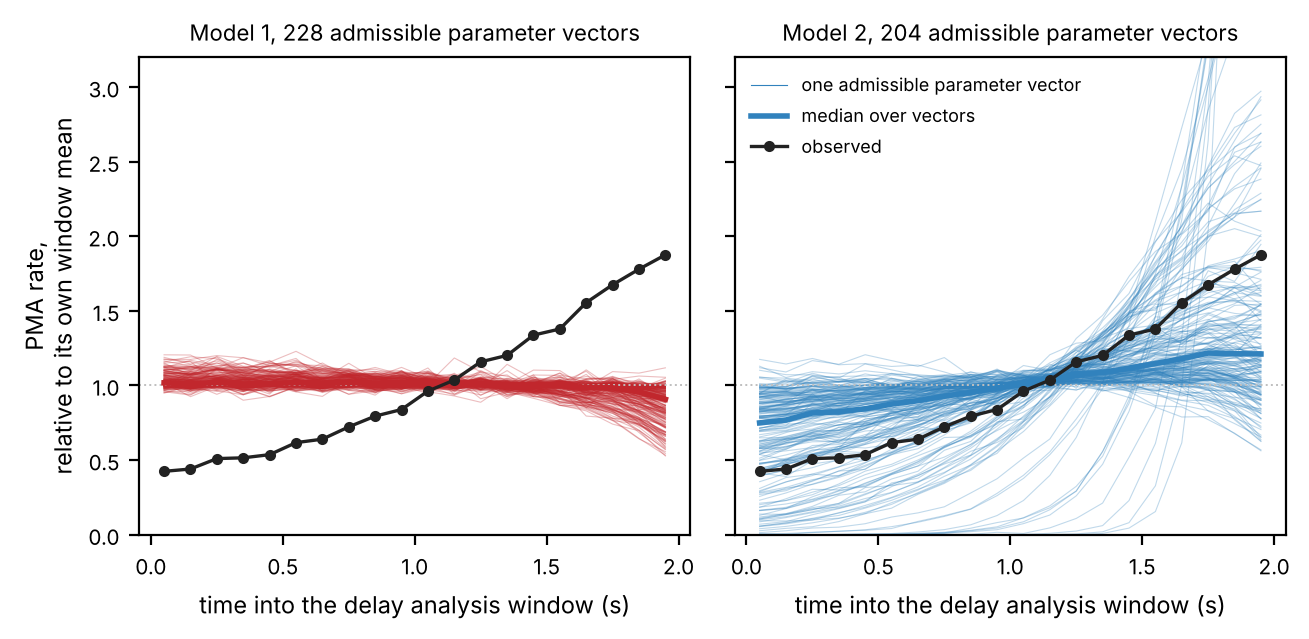
\includegraphics[width=\linewidth]{figures/fig07.png}\end{center}

\begin{center}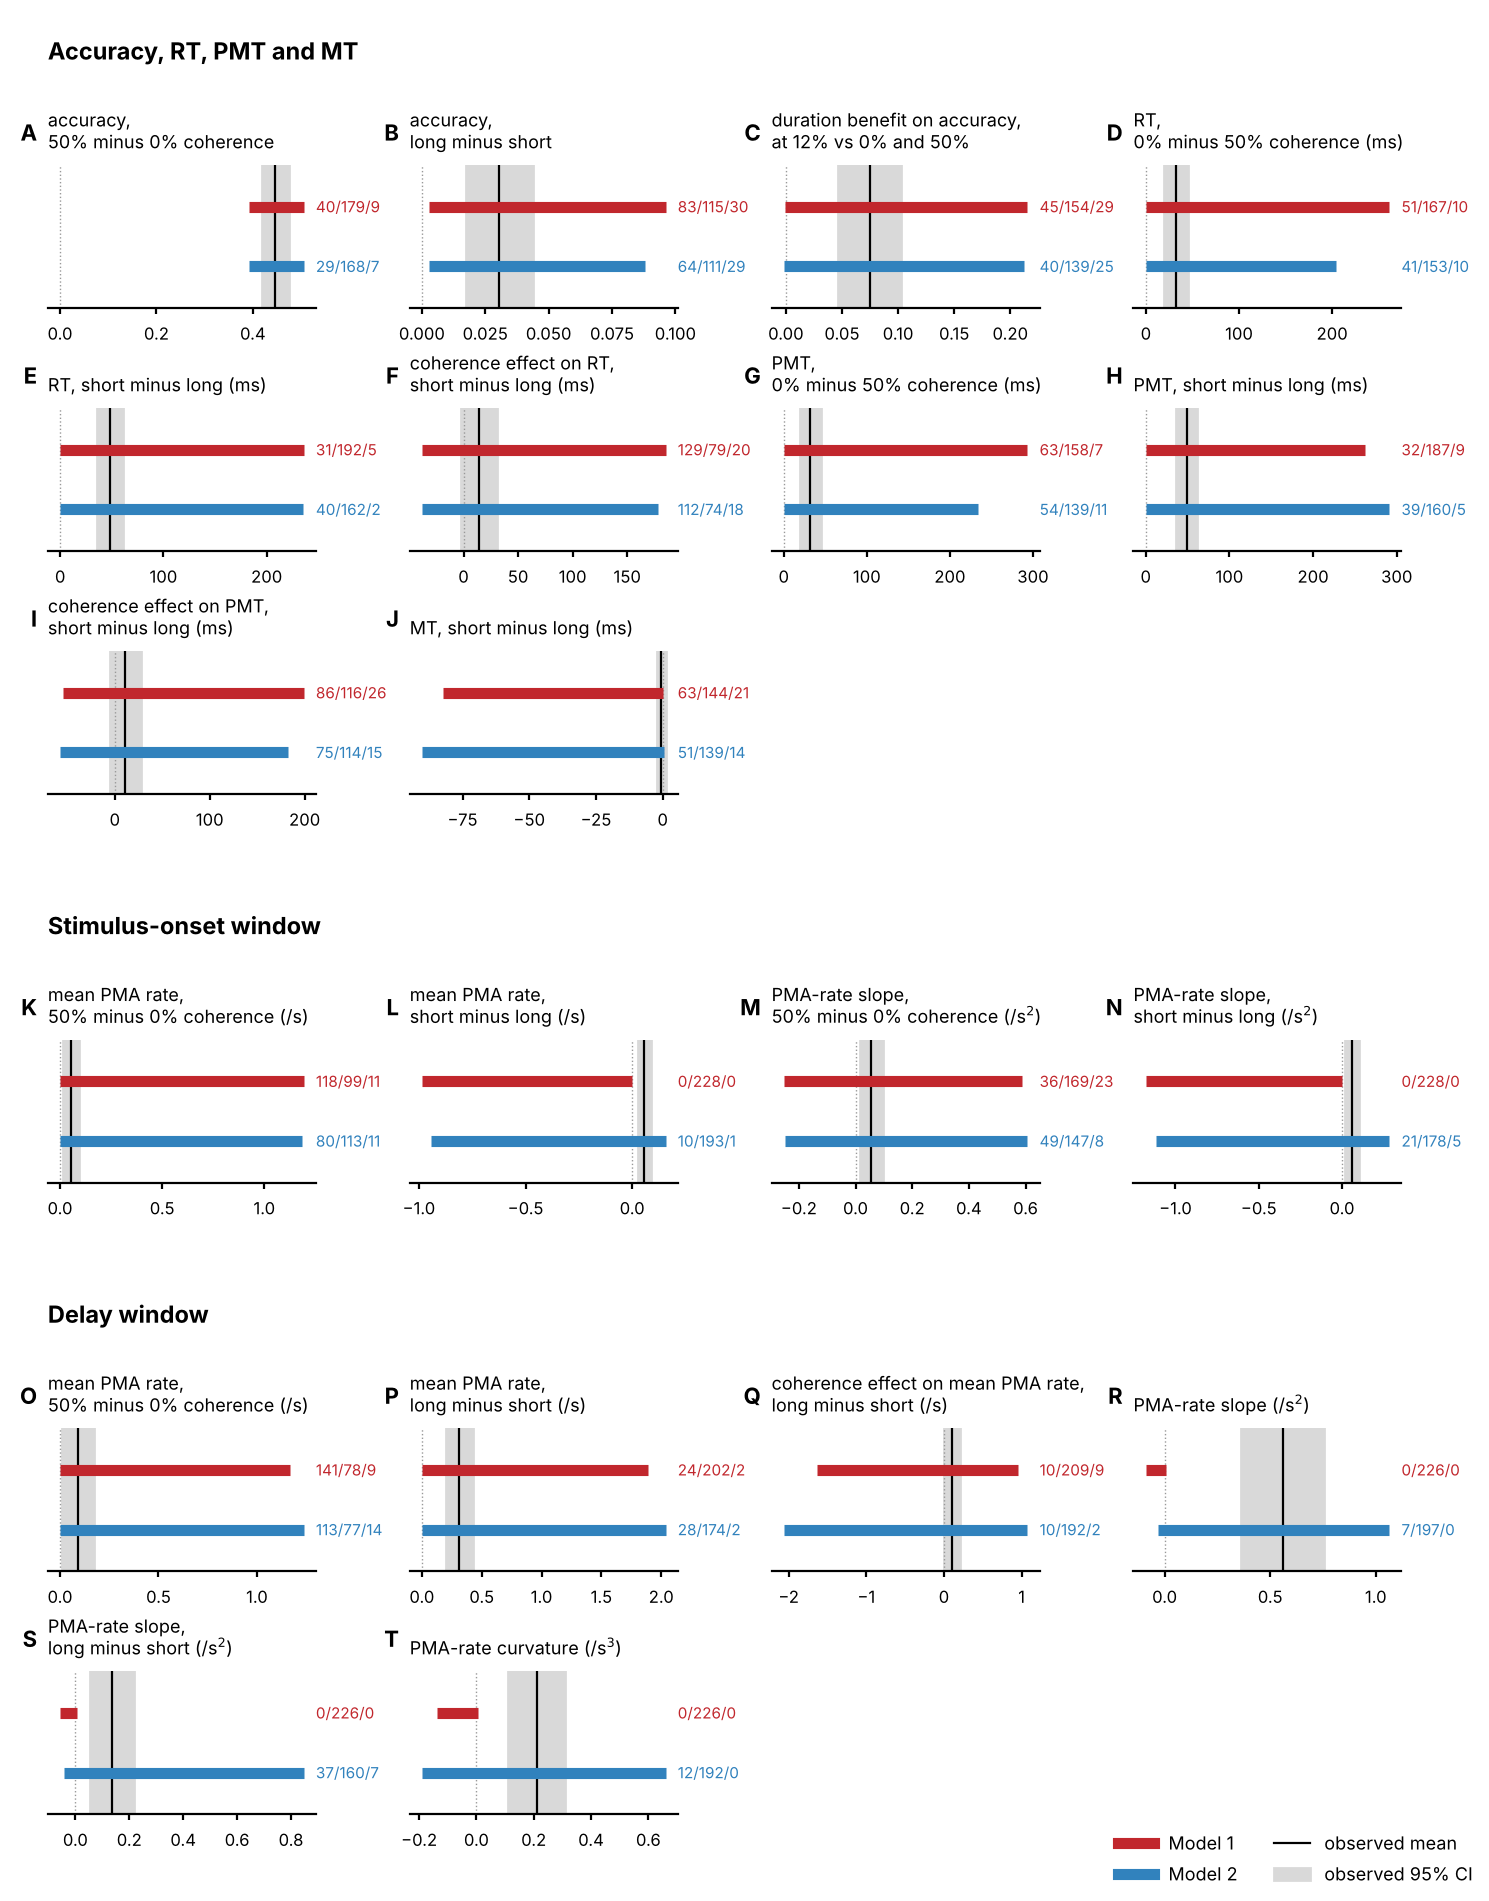
\includegraphics[width=\linewidth]{figures/fig08.png}\end{center}

\new{\emph{Fig S2.}} \new{\emph{The shape prediction of the Appendix, on data alone}}\new{\emph{. Left, the six delay-period log-rate profiles. Right, the log-rate slope falls as a cell's rate rises, as the theory requires, since a higher rate means a smaller distance to the gate. Open symbols: 0.3-s stimulus; filled: 2-s stimulus.}}

\begin{center}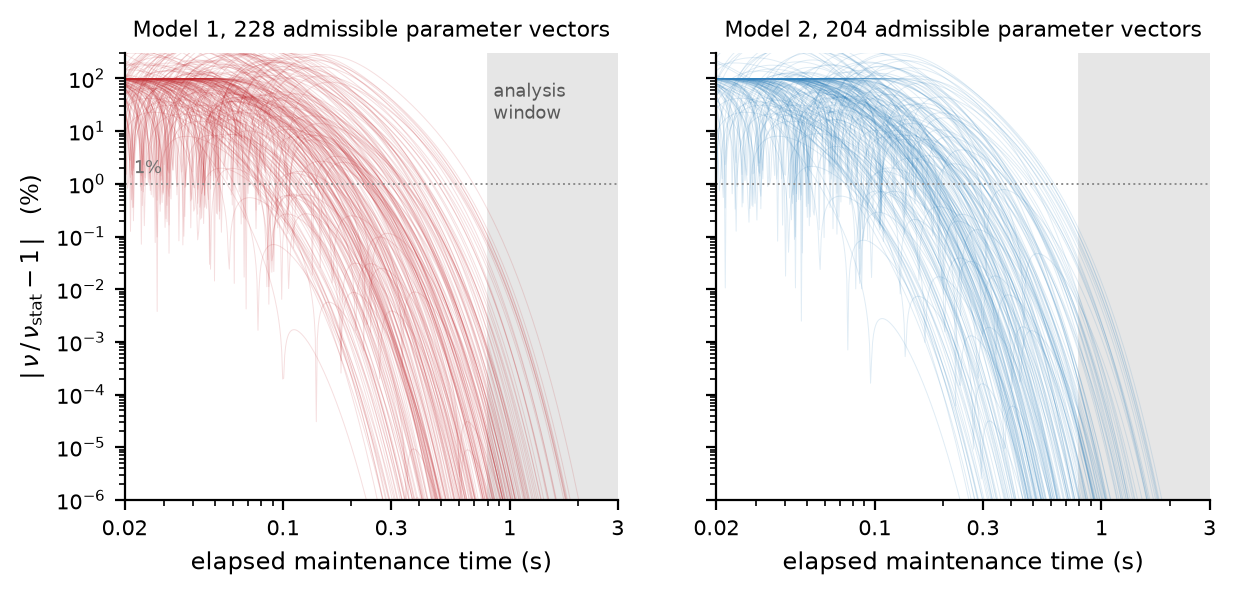
\includegraphics[width=\linewidth]{figures/fig09.png}\end{center}

\new{\textbf{\emph{Fig S3. The ramp--rate frontier, with the sampled parameter space on it. Horizontal axis, the delay-period partial-activation rate (logarithmic); vertical axis, the slope of its logarithm.}}} \new{\textbf{\emph{The red curve is the largest slope Model 1 can attain at each rate, computed in closed form from the kernel over the ranges of Table A1 (Appendix, A.5); the shaded region above it is unreachable by that architecture. Model 2's frontier, computed the same way with the barrier moving and the ramp bounded at the upper quartile of the admissible values, lies far above the panel and is annotated rather than drawn:}}} \new{\textbf{\emph{at the observed rate it reaches +4.05 s\textsuperscript{-1}, against Model 1's 0.000 and an observed +0.89.}}} \new{\textbf{\emph{Open circles are the admissible draws of each model,}}} \new{\textbf{\emph{and the star the observation}}}\new{\textbf{\emph{, with the horizontal bar spanning the observed participant $\times$ condition rates and the grey band the observed slope range.}}}

\begin{center}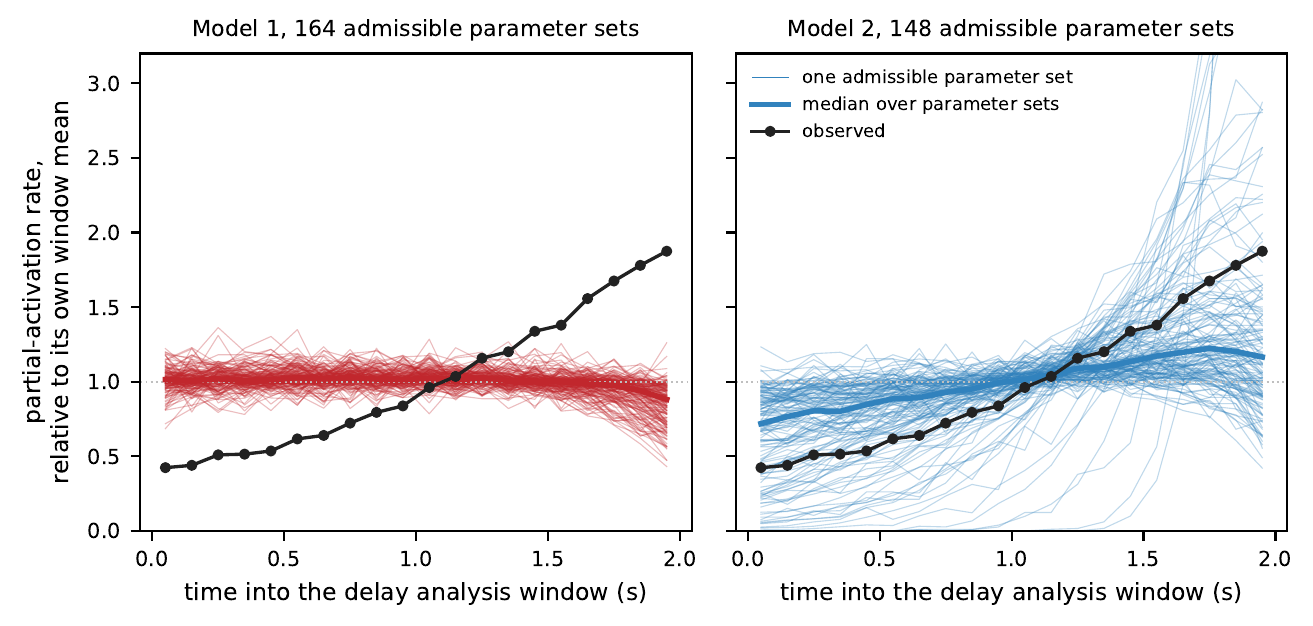
\includegraphics[width=\linewidth]{figures/fig10.png}\end{center}

\new{\textbf{\emph{Fig S4. The shape of the delay-period rate curve, one line per admissible parameter set. Each thin line is the delay-period profile of one admissible set divided by its own mean over the window, so that sets whose rates differ by two orders of magnitude are comparable on shape; the thick line is the median over sets and the black points the observed profile, normalised the same way. The family rather than a summary is the point: the question is whether the architecture can produce the observed rise at all, and the median of a family this wide answers a different one. Every admissible set of Model 1 is flat or declining; Model 2's fan out, many of them tracking the observed rise and beyond.}}}

\begin{center}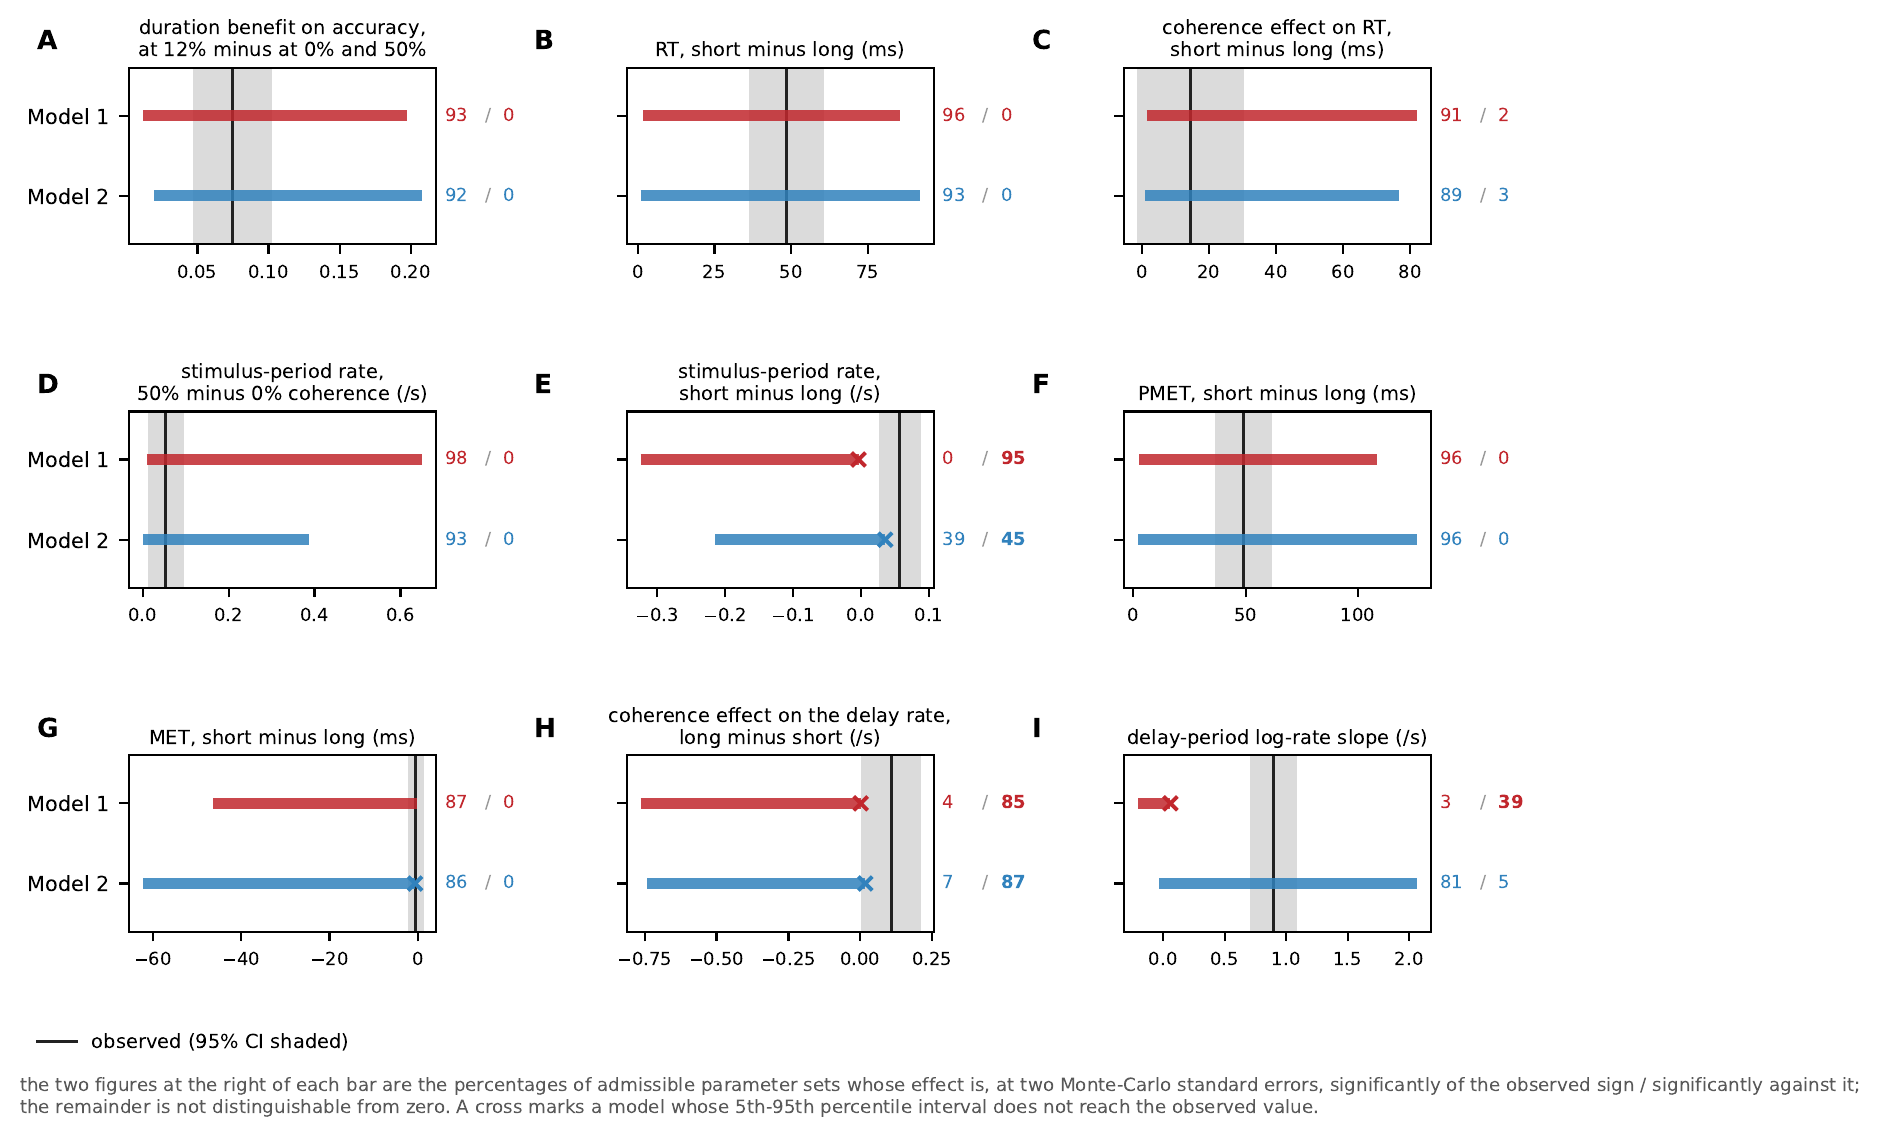
\includegraphics[width=\linewidth]{figures/fig11.png}\end{center}

\new{\textbf{\emph{Fig S5. Effect sizes each architecture can produce, against the observed value,}}} \new{\textbf{\emph{for the nine directional predictions the Results test}}}\new{\textbf{\emph{. Each is written so that the sign the corresponding proposition predicts is positive, and the panel title says which difference is taken. The bar spans the 5th to 95th percentile of that effect over the admissible parameter sets of each model; the vertical line is the observed value and the grey band its 95\% confidence interval across participants; a cross marks a percentile band that does not contain the observed value --- which is not the same as an effect the architecture cannot reach, and on the stimulus-period duration effect and on motor execution time it is not.}}}

\new{The two figures at the right of each bar are the percentages of admissible sets whose effect is, at two Monte-Carlo standard errors, significantly of the observed sign and significantly against it; the remainder is not distinguishable from zero. They measure agreement with the DATA and not with the model's own prediction, and on the coherence $\times$ duration interaction in the delay period the two are opposite: there the 85\% and 87\% counted as against the observed sign are settings at which each architecture does what the saturation argument says it should. Two effects separate the architectures --- the stimulus-period duration effect, where Model 1 has the observed sign at no setting and the opposite sign at 95\% against Model 2's 39\% and 45\%, and the delay-period log-rate slope, at 3\% against 81\%. One is missed by both, the delay-period interaction (4\% and 7\% right against 85\% and 87\% wrong). Of the remaining six, all are reproduced by both at 86\% or above with almost no setting of either model in the opposite direction. The duration effect on motor execution time is a predicted null and is where both architectures are mildly but systematically off: the observed $-$0.5 $\pm$ 0.8 ms is indistinguishable from zero, whereas the models place it significantly below zero at 87\% and 86\% of their settings, with medians of $-$5 and $-$8 ms. The residual motor time is not quite as inert in the simulation as it is in the data.}

\new{\textbf{Table S1. Full ANOVA results for response accuracy, mean response time (RT), mean pre-motor execution time (PMET), and mean motor execution time (MET). Two-way within-subject analyses of variance (duration $\times$ coherence, n = 22), Greenhouse--Geisser corrected wherever a factor has more than two levels, which is why those degrees of freedom are fractional; $\eta$p\textsuperscript{2} is the partial eta squared. Computed by run\_stats.R from the archive's own per-participant $\times$ cell exports.}}

\begin{center}\small
\resizebox{\ifdim\width>\linewidth\linewidth\else\width\fi}{!}{%
\begin{tabular}{llllllll}
\toprule
Dependent variable & Effect tested &  & df1 & df2 & \emph{F} & \emph{p}-value & \emph{$\eta$}\emph{\textsubscript{p}}\emph{\textsuperscript{2}} \\ \midrule
Accuracy & duration &  & \new{1} & \new{21} & \new{22.676} & \new{\emph{p < .001}} & \new{0.519} \\
 & coherence &  & \new{1.30} & \new{27.40} & \new{222.223} & \new{\emph{p < .001}} & \new{0.914} \\
 & duration $\times$ coherence &  & \new{1.96} & \new{41.24} & \new{12.171} & \new{\emph{p < .001}} & \new{0.367} \\
 &  &  &  &  &  &  &  \\
Mean RT & duration &  & \new{1} & \new{21} & \new{65.790} & \new{\emph{p < .001}} & \new{0.758} \\
 & coherence &  & \new{1.49} & \new{31.39} & \new{14.190} & \new{\emph{p < .001}} & \new{0.403} \\
 & duration $\times$ coherence &  & \new{1.68} & \new{35.25} & \new{4.607} & \new{\emph{p = .022}} & \new{0.180} \\
 &  &  &  &  &  &  &  \\
Mean PMET & duration &  & \new{1} & \new{21} & \new{69.600} & \new{\emph{p < .001}} & \new{0.768} \\
 & coherence &  & \new{1.60} & \new{33.50} & \new{14.000} & \new{\emph{p < .001}} & \new{0.400} \\
 & duration $\times$ coherence &  & \new{1.72} & \new{36.14} & \new{3.575} & \new{\emph{p = .045}} & \new{0.145} \\
 &  &  &  &  &  &  &  \\
Mean MET & duration &  & \new{1} & \new{21} & \new{1.095} & \new{\emph{p = .307}} & \new{0.050} \\
 & coherence &  & \new{1.51} & \new{31.73} & \new{0.624} & \new{\emph{p = .499}} & \new{0.029} \\
 & duration $\times$ coherence &  & \new{1.86} & \new{39.12} & \new{2.436} & \new{\emph{p = .104}} & \new{0.104} \\
\bottomrule
\end{tabular}
}
\end{center}
\emph{Note}.  A partial eta squared statistic  (\emph{$\eta$}\emph{\textsubscript{p}}\emph{\textsuperscript{2}})  is reported as a measure of effect size. Degrees of freedom (df) with decimals indicate that a Greenhouse-Geisser correction was applied.

\textbf{Table S2}\textbf{.} \textbf{Full ANOVA results for} \textbf{partial muscle activation rate in the electromyographic channel of the responding effector}  \textbf{across} \textbf{task periods}\textbf{.}

\begin{center}\small
\resizebox{\ifdim\width>\linewidth\linewidth\else\width\fi}{!}{%
\begin{tabular}{lllllll}
\toprule
Period & Effect tested & df1 & df2 & \emph{F} & \emph{p}-value & \emph{$\eta$}\emph{\textsubscript{p}}\emph{\textsuperscript{2}} \\ \midrule
Stimulus & duration & 1 & 21 & \new{13.381} & \emph{p} =  .001 & 0.389 \\
 & coherence & 1.33 & 28.01 & \new{5.251} & \emph{p} =  .021 & 0.200 \\
 & time, linear & \new{1} & \new{21} & \new{30.869} & p < .001 & \new{0.595} \\
 & duration $\times$ coherence & \new{1.98} & \new{41.51} & 0.312 & \new{\emph{p = .731}} & -- \\
 & duration $\times$ time, linear & \new{1} & \new{21} & \new{9.532} & \new{p = .006} & \new{0.312} \\
 & coherence $\times$ time, linear & \new{1.72} & \new{36.20} & \new{6.145} & \new{p = .007} & \new{0.226} \\
 & duration $\times$ coherence $\times$ time, linear & \new{1.87} & \new{39.18} & \new{0.729} & \new{p = .480} & \new{0.034} \\
 & time, quadratic & \new{1} & \new{21} & 2.621 & p = .120 & 0.111 \\
 & duration $\times$ time, quadratic & \new{1} & \new{21} & 3.555 & p = .073 & 0.145 \\
 & coherence $\times$ time, quadratic & 1.90 & 39.81 & 0.525 & p = .586 & 0.024 \\
 & duration $\times$ coherence $\times$ time, quadratic & 1.59 & 33.42 & 0.403 & p = .625 & 0.019 \\
 &  &  &  &  &  &  \\
Delay & duration & 1 & 21 & \new{33.186} & \emph{p}  < .001 & 0.612 \\
 & coherence & \new{1.96} & \new{41.15} & \new{3.361} & \new{\emph{p = .045}} & 0.138 \\
 & time, linear & \new{1} & \new{21} & \new{35.238} & p < .001 & \new{0.627} \\
 & duration $\times$ coherence & \new{1.92} & \new{40.42} & 3.474 & \new{\emph{p = .042}} & 0.142 \\
 & duration $\times$ time, linear & \new{1} & \new{21} & \new{11.898} & \new{p = .002} & \new{0.362} \\
 & coherence $\times$ time, linear & \new{1.70} & \new{35.61} & \new{0.524} & \new{p = .567} & \new{0.024} \\
 & duration $\times$ coherence $\times$ time, linear & \new{1.74} & \new{36.45} & \new{0.508} & \new{p = .580} & \new{0.024} \\
 & time, quadratic & \new{1} & \new{21} & 18.891 & p < .001 & 0.474 \\
 & duration $\times$ time, quadratic & \new{1} & \new{21} & 0.751 & p = .396 & 0.035 \\
 & coherence $\times$ time, quadratic & 1.95 & 40.89 & 1.855 & p = .170 & 0.081 \\
 & duration $\times$ coherence $\times$ time, quadratic & 1.86 & 39.04 & 0.946 & p = .391 & 0.043 \\
 &  &  &  &  &  &  \\
Response signal & duration & 1 & 21 & \new{36.559} & \emph{p}  < .001 & 0.635 \\
 & coherence & 1.56 & 32.82 & 1.159 & \emph{p} =  .315 & -- \\
 & time & 1 & 21 & \new{21.964} & \emph{p}  < .001 & 0.511 \\
 & duration $\times$ coherence & \new{1.91} & \new{40.04} & 0.041 & \new{\emph{p = .954}} & -- \\
 & duration $\times$ time & 1 & 21 & 7.046 & \emph{p} =  .015 & 0.251 \\
 & coherence $\times$ time & \new{1.84} & \new{38.61} & 0.407 & \new{\emph{p = .651}} & -- \\
 & duration $\times$ coherence $\times$ time & \new{1.75} & \new{36.67} & 0.587 & \new{\emph{p = .539}} & -- \\
 &  &  &  &  &  &  \\
Response & \new{duration} & \new{1} & \new{21} & \new{7.613} & \new{p = .012} & \new{0.266} \\
Response & \new{coherence} & \new{1.90} & \new{39.98} & \new{1.845} & \new{p = .173} & \new{0.081} \\
Response & \new{duration $\times$ coherence} & \new{1.86} & \new{39.10} & \new{0.342} & \new{p = .697} & \new{0.016} \\
\bottomrule
\end{tabular}
}
\end{center}
\new{Note. Greenhouse--Geisser correction was applied to every effect with more than one numerator degree of freedom, that is to every effect involving the three-level coherence factor; degrees of freedom (df) with decimals indicate a corrected test. The partial eta squared statistic ($\eta$p2) is computed from the uncorrected degrees of freedom and is therefore unchanged by that correction. Time refers to the time bin factor. The time-bin main effect and its interactions are reported as one-degree-of-freedom linear-trend and quadratic contrasts computed on per-participant scores for the Stimulus and Delay periods (Methods): a contrast crossed only with duration therefore yields F(1,21), whereas a contrast crossed with coherence carries corrected degrees of freedom. The RS period is unaffected (only two time bins, so the omnibus and trend tests coincide exactly, and no quadratic contrast exists). The Response period is analyzed on its single informative bin, for which no time-bin factor --- and therefore no trend or quadratic decomposition --- applies (Methods).}

\textbf{Table} \textbf{S2}\textbf{.} \textbf{Full ANOVA results for} \textbf{the} \textbf{late}\textbf{ralized readiness potential} \textbf{amplitude}  \textbf{across} \textbf{task periods}\textbf{.}

\begin{center}\small
\resizebox{\ifdim\width>\linewidth\linewidth\else\width\fi}{!}{%
\begin{tabular}{llllllll}
\toprule
Period & Effect tested &  & df1 & df2 & \emph{F} & \emph{p}-value & \emph{$\eta$}\emph{\textsubscript{p}}\emph{\textsuperscript{2}} \\ \midrule
Stimulus & duration &  & 1 & 21 & \new{0.614} & \new{\emph{p = .442}} & -- \\
 & coherence &  & \new{1.75} & \new{36.66} & \new{1.498} & \new{\emph{p = .237}} & -- \\
 & time, linear &  & \new{1} & \new{21} & \new{0.497} & \new{p = .489} & \new{0.023} \\
 & duration $\times$ coherence &  & \new{1.87} & \new{39.26} & \new{0.387} & \new{\emph{p = .668}} & -- \\
 & duration $\times$ time, linear &  & \new{1} & \new{21} & \new{2.222} & \new{p = .151} & \new{0.096} \\
 & coherence $\times$ time, linear &  & \new{1.49} & \new{31.27} & \new{0.551} & \new{p = .531} & \new{0.026} \\
 & duration $\times$ coherence $\times$ time, linear &  & \new{1.97} & \new{41.44} & \new{0.169} & \new{p = .843} & \new{0.008} \\
 & time, quadratic &  & \new{1} & \new{21} & 0.487 & p = .493 & 0.023 \\
 & duration $\times$ time, quadratic &  & \new{1} & \new{21} & 7.201 & p = .014 & 0.255 \\
 & coherence $\times$ time, quadratic &  & 1.74 & 36.63 & 2.267 & p = .124 & 0.097 \\
 & duration $\times$ coherence $\times$ time, quadratic &  & 1.93 & 40.61 & 0.161 & p = .845 & 0.008 \\
 &  &  &  &  &  &  &  \\
Delay & duration &  & 1 & 21 & 0.019 & \emph{p} =  .892 & -- \\
 & coherence &  & 1.34 & 28.13 & \new{0.440} & \emph{p} =  .569 & -- \\
 & time, linear &  & \new{1} & \new{21} & \new{14.338} & p = .001 & \new{0.406} \\
 & duration $\times$ coherence &  & \new{1.96} & \new{41.16} & 0.378 & \new{\emph{p = .683}} & -- \\
 & duration $\times$ time, linear &  & \new{1} & \new{21} & \new{0.262} & \new{p = .614} & \new{0.012} \\
 & coherence $\times$ time, linear &  & \new{1.56} & \new{32.72} & \new{0.283} & \new{p = .701} & \new{0.013} \\
 & duration $\times$ coherence $\times$ time, linear &  & \new{1.90} & \new{39.84} & \new{0.031} & \new{p = .964} & \new{0.001} \\
 & time, quadratic &  & \new{1} & \new{21} & 4.041 & p = .057 & 0.161 \\
 & duration $\times$ time, quadratic &  & \new{1} & \new{21} & 0.574 & p = .457 & 0.027 \\
 & coherence $\times$ time, quadratic &  & 1.93 & 40.62 & 0.682 & p = .506 & 0.031 \\
 & duration $\times$ coherence $\times$ time, quadratic &  & 1.98 & 41.67 & 0.330 & p = .719 & 0.015 \\
 &  &  &  &  &  &  &  \\
Response signal & duration &  & 1 & 21 & 0.185 & \emph{p} =  .671 & -- \\
 & coherence &  & 1.45 & 30.43 & 0.252 & \emph{p} =  .707 & -- \\
 & time &  & 1 & 21 & 14.076 & \emph{p} =  .001 & 0.401 \\
 & duration $\times$ coherence &  & \new{1.96} & \new{41.08} & 0.267 & \new{\emph{p = .762}} & -- \\
 & duration $\times$ time &  & 1 & 21 & 1.238 & \emph{p} =  .278 & -- \\
 & coherence $\times$ time &  & \new{1.59} & \new{33.39} & 1.058 & \new{\emph{p = .344}} & -- \\
 & duration $\times$ coherence $\times$ time &  & \new{1.94} & \new{40.83} & 0.108 & \new{\emph{p = .893}} & -- \\
 &  &  &  &  &  &  &  \\
Response & duration &  & 1 & 21 & \new{0.400} & \emph{p} =  .534 & -- \\
 & coherence &  & 1.55 & 32.45 & \new{0.309} & \emph{p} =  .680 & -- \\
 & time &  & 1 & 21 & 54.331 & \emph{p}  < .001 & 0.721 \\
 & duration $\times$ coherence &  & \new{1.97} & \new{41.30} & 0.666 & \new{\emph{p = .517}} & -- \\
 & duration $\times$ time &  & 1 & 21 & 4.129 & \emph{p} =  .055 & -- \\
 & coherence $\times$ time &  & \new{1.60} & \new{33.70} & 0.246 & \new{\emph{p = .734}} & -- \\
 & duration $\times$ coherence $\times$ time &  & \new{1.62} & \new{34.05} & 0.589 & \new{\emph{p = .526}} & -- \\
\bottomrule
\end{tabular}
}
\end{center}
\new{Note. Greenhouse--Geisser correction was applied to every effect with more than one numerator degree of freedom, that is to every effect involving the three-level coherence factor; degrees of freedom (df) with decimals indicate a corrected test. The partial eta squared statistic ($\eta$p2) is computed from the uncorrected degrees of freedom and is therefore unchanged by that correction. Time refers to the time bin factor. The time-bin main effect and its interactions are reported as one-degree-of-freedom linear-trend and quadratic contrasts computed on per-participant scores for the Stimulus and Delay periods (Methods): a contrast crossed only with duration therefore yields F(1,21), whereas a contrast crossed with coherence carries corrected degrees of freedom. The RS and Response periods are unaffected (two time bins each, so the omnibus and trend tests coincide exactly, and no quadratic contrast exists).}

\textbf{Table} \textbf{S3.} \textbf{Full ANOVA results} \textbf{for} \textbf{mu--beta-band spectral amplitude lateralization} \textbf{across} \textbf{task periods}\textbf{.}

\begin{center}\small
\resizebox{\ifdim\width>\linewidth\linewidth\else\width\fi}{!}{%
\begin{tabular}{llllllll}
\toprule
Period & Effect tested &  & df1 & df2 & \emph{F} & \emph{p}-value & \emph{$\eta$}\emph{\textsubscript{p}}\emph{\textsuperscript{2}} \\ \midrule
Stimulus & duration &  & 1 & 21 & 2.146 & \emph{p} =  .158 & -- \\
 & coherence &  & 1.31 & 27.56 & 2.813 & \emph{p} =  .096 & -- \\
 & time, linear &  & \new{1} & \new{21} & \new{11.740} & \new{p = .003} & \new{0.359} \\
 & duration $\times$ coherence &  & \new{1.62} & \new{34.00} & 0.755 & \new{\emph{p = .452}} & -- \\
 & duration $\times$ time, linear &  & \new{1} & \new{21} & \new{4.497} & \new{p = .046} & \new{0.176} \\
 & coherence $\times$ time, linear &  & \new{1.95} & \new{40.99} & \new{0.517} & \new{p = .596} & \new{0.024} \\
 & duration $\times$ coherence $\times$ time, linear &  & \new{1.85} & \new{38.90} & \new{0.021} & \new{p = .974} & \new{0.001} \\
 & time, quadratic &  & \new{1} & \new{21} & 9.116 & p = .007 & 0.303 \\
 & duration $\times$ time, quadratic &  & \new{1} & \new{21} & 0.236 & p = .632 & 0.011 \\
 & coherence $\times$ time, quadratic &  & 1.66 & 34.89 & 1.936 & p = .165 & 0.084 \\
 & duration $\times$ coherence $\times$ time, quadratic &  & 1.99 & 41.79 & 1.302 & p = .283 & 0.058 \\
 &  &  &  &  &  &  &  \\
Delay & duration &  & 1 & 21 & 3.177 & \emph{p} =  .089 & -- \\
 & coherence &  & 1.29 & 27.12 & 1.257 & \emph{p} =  .285 & -- \\
 & time, linear &  & \new{1} & \new{21} & \new{7.107} & \new{p = .014} & \new{0.253} \\
 & duration $\times$ coherence &  & \new{1.69} & \new{35.43} & 1.586 & \new{\emph{p = .220}} & -- \\
 & duration $\times$ time, linear &  & \new{1} & \new{21} & \new{0.019} & \new{p = .893} & \new{0.001} \\
 & coherence $\times$ time, linear &  & \new{1.78} & \new{37.43} & \new{1.371} & \new{p = .265} & \new{0.061} \\
 & duration $\times$ coherence $\times$ time, linear &  & \new{1.81} & \new{37.91} & \new{2.687} & \new{p = .086} & \new{0.113} \\
 & time, quadratic &  & \new{1} & \new{21} & 3.290 & p = .084 & 0.135 \\
 & duration $\times$ time, quadratic &  & \new{1} & \new{21} & 3.741 & p = .067 & 0.151 \\
 & coherence $\times$ time, quadratic &  & 1.96 & 41.11 & 3.147 & p = .054 & 0.130 \\
 & duration $\times$ coherence $\times$ time, quadratic &  & 1.29 & 27.01 & 0.565 & p = .501 & 0.026 \\
 &  &  &  &  &  &  &  \\
Response signal & duration &  & 1 & 21 & 3.039 & \emph{p} =  .096 & -- \\
 & coherence &  & \new{1.90} & \new{39.94} & \new{0.160} & \new{\emph{p = .843}} & -- \\
 & time &  & 1 & 21 & 0.059 & \emph{p} =  .810 & -- \\
 & duration $\times$ coherence &  & \new{2.00} & \new{41.96} & 1.216 & \emph{p} =  .307 & -- \\
 & duration $\times$ time &  & 1 & 21 & 1.509 & \emph{p} =  .233 & -- \\
 & coherence $\times$ time &  & \new{1.99} & \new{41.73} & 0.024 & \new{\emph{p = .976}} & -- \\
 & duration $\times$ coherence $\times$ time &  & \new{1.66} & \new{34.93} & 1.458 & \new{\emph{p = .246}} & -- \\
 &  &  &  &  &  &  &  \\
Response & duration &  & 1 & 21 & 0.006 & \emph{p} =  .937 & -- \\
 & coherence &  & \new{1.95} & \new{40.91} & 0.364 & \new{\emph{p = .692}} & -- \\
 & time &  & 1 & 21 & \new{11.658} & \emph{p}  = .003 & 0.357 \\
 & duration $\times$ coherence &  & \new{1.65} & \new{34.56} & 0.161 & \new{\emph{p = .811}} & -- \\
 & duration $\times$ time &  & 1 & 21 & 2.129 & \emph{p} =  .159 & -- \\
 & coherence $\times$ time &  & \new{1.98} & \new{41.51} & 0.252 & \new{\emph{p = .776}} & -- \\
 & duration $\times$ coherence $\times$ time &  & \new{1.72} & \new{36.21} & 0.719 & \new{\emph{p = .475}} & -- \\
\bottomrule
\end{tabular}
}
\end{center}
\new{Note. Greenhouse--Geisser correction was applied to every effect with more than one numerator degree of freedom, that is to every effect involving the three-level coherence factor; degrees of freedom (df) with decimals indicate a corrected test. The partial eta squared statistic ($\eta$p2) is computed from the uncorrected degrees of freedom and is therefore unchanged by that correction. Time refers to the time bin factor. The time-bin main effect and its interactions are reported as one-degree-of-freedom linear-trend and quadratic contrasts computed on per-participant scores for the Stimulus and Delay periods (Methods): a contrast crossed only with duration therefore yields F(1,21), whereas a contrast crossed with coherence carries corrected degrees of freedom. One stimulus-period effect (coherence $\times$ time, linear) is significant on the omnibus test but not as a full-window linear trend, because the effect is confined to the first half of the stimulus period (Results; Table S4). One other (duration $\times$ time, linear) is significant as a linear trend but was not significant on the omnibus test. The RS and Response periods are unaffected (two time bins each, so the omnibus and trend tests coincide exactly, and no quadratic contrast exists).}

\textbf{Table S4.} \textbf{Mu--beta lateralization, stimulus period: split-half trend analysis.}

\new{A non-monotone profile for this measure was anticipated in Methods (rising over approximately the first second of the stimulus period and flattening thereafter), which is why a quadratic contrast was prespecified alongside the linear one. To characterize this directly, the stimulus period was split a priori at its temporal midpoint into two 1-s halves (bins 1--10 and 11--20) and the same TREND analysis was repeated within each half:}

\begin{center}\small
\resizebox{\ifdim\width>\linewidth\linewidth\else\width\fi}{!}{%
\begin{tabular}{lllllll}
\toprule
\new{Window} & \new{trend F} & \new{trend p} & \new{trend $\times$ coherence F} & \new{trend $\times$ coherence p} & \new{trend $\times$ duration F} & \new{trend $\times$ duration p} \\ \midrule
\new{first half (0--1 s)} & \new{11.19} & \new{.003} & \new{5.76} & \new{.018} & \new{5.67} & \new{.027} \\
\new{second half (1--2 s)} & \new{2.22} & \new{.151} & \new{0.37} & \new{.658} & \new{5.34} & \new{.031} \\
\bottomrule
\end{tabular}
}
\end{center}
\new{The coherence-dependent trend is present in the first half (linear trend $\times$ coherence significant) and extinguished in the second half (same contrast null), while the duration-dependent trend holds in both halves. This is the pattern expected if coherence-dependent trajectories are converging on a common sustained level rather than ramping at a constant, coherence-dependent rate throughout the period: the full-window test in Table S3 above, which averages across both halves, accordingly shows neither a significant linear nor quadratic coherence $\times$ time trend.}

\textbf{Table S5.} \textbf{Delay-period partial-activation rate: an unbinned point-process analysis.}

\new{To avoid the arbitrary time-bin factor altogether (Materials and Methods), the coherence-dependent ramp in delay-period partial-activation rate was additionally tested with no binning at all, using the exact onset time of each partial activation. Writing the log-intensity as a linear function of time,} $\ln \nu \left(t\right)={c}_{0}+{c}_{1}t$\new{, the log-rate slope} ${c}_{1}$ \new{was estimated per participant and per coherence $\times$ duration cell from an inhomogeneous-Poisson point-process likelihood and entered into the same repeated-measures ANOVA as any other score (two-stage estimator); a one-stage log-linear model fitted across all participants with cluster-robust standard errors gave the same pattern of results (below). Both estimators treat the Poisson likelihood as a quasi-likelihood rather than a literal one, since upcrossing events cluster in time; standard errors accordingly come from between-participant variation (two-stage) or a cluster-robust correction (one-stage). This is a different estimator from the binned one the bound of the Appendix is compared against (Appendix, A.7), which must match the binning of the published analysis; the two agree on the sign and the approximate size of the slope.}

\begin{center}\small
\resizebox{\ifdim\width>\linewidth\linewidth\else\width\fi}{!}{%
\begin{tabular}{lll}
\toprule
 & \new{two-stage} & \new{one-stage, robust} \\ \midrule
\new{log-rate slope} & \new{+0.929, F(1,21) = 102.95, p < .001} & \new{+0.841, z = 11.23, p < .001} \\
\new{slope $\times$ duration} & \new{F(1,21) = 4.78, p = .040} & \new{$-$0.179, z = $-$3.17, p = .002} \\
\new{slope $\times$ coherence} & \new{F(1.38,29.04) = 4.20, p = .038} & \new{$-$0.263, z = $-$5.02, p < .001} \\
\new{slope $\times$ duration $\times$ coherence} & \new{F(1.87,39.23) = 0.39, p = .663} & \new{---} \\
\bottomrule
\end{tabular}
}
\end{center}
\new{The log-rate slope was positive and shallower both after a long stimulus and at high coherence --- the pattern expected under accumulation to an internal threshold, since either factor raises the maintained level and thereby} \new{reduces the distance to the gate (}\new{Equation (25)}\new{).} \new{The two estimators agree on sign throughout and differ in magnitude by about a tenth, consistent with the two-stage estimator weighting participants equally and the one-stage estimator weighting them by precision.}

\end{document}
